\documentclass[11pt]{article}
\usepackage[margin=1in]{geometry}
\usepackage[T1]{fontenc}
\usepackage{lmodern}
\usepackage{amsmath,amssymb}
\usepackage{graphicx}
\usepackage{booktabs}
\usepackage{float}
\usepackage{verbatim}
\usepackage{xcolor}
\usepackage{url}
\usepackage[numbers,sort&compress]{natbib}
\usepackage[colorlinks=true,linkcolor=black,citecolor=blue!50!black,urlcolor=blue!50!black]{hyperref}
% generated by src/make_numbers.py; do not edit
\newcommand{\NumTotalSteps}{74}
\newcommand{\NumTotalSig}{20}
\newcommand{\NumTotalHolm}{13}
\newcommand{\NumTotalSigPct}{27}
\newcommand{\NumTotalNotSigPct}{73}
\newcommand{\NumTotalHolmPct}{18}
\newcommand{\NumTotalTwoSided}{20}
\newcommand{\NumTotalTwoSidedPct}{27}
\newcommand{\NumTotalOneSided}{25}
\newcommand{\NumTotalOneSidedPct}{34}
\newcommand{\NumWorstSteps}{99}
\newcommand{\NumWorstSig}{29}
\newcommand{\NumWorstSigPct}{29}
\newcommand{\NumSmallSteps}{61}
\newcommand{\NumSmallSig}{11}
\newcommand{\NumSmallHolm}{4}
\newcommand{\NumSmallSigPct}{18}
\newcommand{\NumSmallHolmPct}{7}
\newcommand{\NumSmallBoards}{5}
\newcommand{\NumLargeSteps}{13}
\newcommand{\NumLargeSig}{9}
\newcommand{\NumSmallMarginSteps}{35}
\newcommand{\NumSmallMarginSig}{0}
\newcommand{\NumClusterSig}{10}
\newcommand{\NumClusterSteps}{65}
\newcommand{\NumClusterSigPct}{15}
\newcommand{\NumSWEIidSig}{19}
\newcommand{\NumBoardsWithSteps}{5}
\newcommand{\NumVerifiedK}{135}
\newcommand{\NumVerifiedT}{500}
\newcommand{\NumVerifiedLeader}{79.2}
\newcommand{\NumVerifiedPBest}{0.35}
\newcommand{\NumVerifiedLeaderTied}{2}
\newcommand{\NumVerifiedSet}{14}
\newcommand{\NumVerifiedSetSim}{20}
\newcommand{\NumVerifiedNoiseRecords}{4.5}
\newcommand{\NumVerifiedWinnerObs}{79.2}
\newcommand{\NumVerifiedWinnerAdj}{78.1}
\newcommand{\NumVerifiedWinnerDrop}{1.1}
\newcommand{\NumVerifiedCondAdj}{undefined}
\newcommand{\NumVerifiedCoLeaders}{2}
\newcommand{\NumVerifiedPBestOther}{0.32}
\newcommand{\NumVerifiedSteps}{30}
\newcommand{\NumVerifiedSig}{6}
\newcommand{\NumVerifiedHolm}{2}
\newcommand{\NumVerifiedTwoSided}{6}
\newcommand{\NumVerifiedOneSided}{7}
\newcommand{\NumVerifiedMedianMargin}{1.5}
\newcommand{\NumVerifiedMedianLag}{2}
\newcommand{\NumVerifiedShareAdjacent}{20}
\newcommand{\NumVerifiedShareNever}{0}
\newcommand{\NumVerifiedUpperNonSig}{4.6}
\newcommand{\NumVerifiedWorstSteps}{36}
\newcommand{\NumVerifiedWorstSig}{9}
\newcommand{\NumVerifiedClusterSig}{1}
\newcommand{\NumVerifiedCritMargin}{3.0}
\newcommand{\NumVerifiedMDD}{4.3}
\newcommand{\NumVerifiedTasksOnePt}{9{,}300}
\newcommand{\NumVerifiedTasksTwoPt}{2{,}300}
\newcommand{\NumVerifiedMDDLo}{3.8}
\newcommand{\NumVerifiedMDDHi}{4.7}
\newcommand{\NumVerifiedTasksOnePtLo}{7{,}100}
\newcommand{\NumVerifiedTasksOnePtHi}{10{,}800}
\newcommand{\NumVerifiedWinnerCiLo}{74.9}
\newcommand{\NumVerifiedWinnerCiHi}{81.5}
\newcommand{\NumVerifiedMDDCluster}{4.8}
\newcommand{\NumVerifiedSetCluster}{21}
\newcommand{\NumVerifiedPBestCluster}{0.37}
\newcommand{\NumLiteK}{84}
\newcommand{\NumLiteT}{300}
\newcommand{\NumLiteLeader}{60.3}
\newcommand{\NumLitePBest}{0.47}
\newcommand{\NumLiteLeaderTied}{1}
\newcommand{\NumLiteSet}{5}
\newcommand{\NumLiteSetSim}{6}
\newcommand{\NumLiteNoiseRecords}{4.0}
\newcommand{\NumLiteWinnerObs}{60.3}
\newcommand{\NumLiteWinnerAdj}{58.7}
\newcommand{\NumLiteWinnerDrop}{1.7}
\newcommand{\NumLiteCondAdj}{55.7}
\newcommand{\NumLiteCoLeaders}{1}
\newcommand{\NumLitePBestOther}{--}
\newcommand{\NumLiteSteps}{15}
\newcommand{\NumLiteSig}{3}
\newcommand{\NumLiteHolm}{1}
\newcommand{\NumLiteTwoSided}{3}
\newcommand{\NumLiteOneSided}{6}
\newcommand{\NumLiteMedianMargin}{3.0}
\newcommand{\NumLiteMedianLag}{2}
\newcommand{\NumLiteShareAdjacent}{20}
\newcommand{\NumLiteShareNever}{0}
\newcommand{\NumLiteUpperNonSig}{7.2}
\newcommand{\NumLiteWorstSteps}{20}
\newcommand{\NumLiteWorstSig}{4}
\newcommand{\NumLiteClusterSig}{1}
\newcommand{\NumLiteCritMargin}{4.7}
\newcommand{\NumLiteMDD}{6.7}
\newcommand{\NumLiteTasksOnePt}{13{,}700}
\newcommand{\NumLiteTasksTwoPt}{3{,}400}
\newcommand{\NumLiteMDDLo}{6.1}
\newcommand{\NumLiteMDDHi}{7.5}
\newcommand{\NumLiteTasksOnePtLo}{11{,}300}
\newcommand{\NumLiteTasksOnePtHi}{17{,}100}
\newcommand{\NumLiteWinnerCiLo}{53.4}
\newcommand{\NumLiteWinnerCiHi}{63.7}
\newcommand{\NumLiteMDDCluster}{6.4}
\newcommand{\NumLiteSetCluster}{9}
\newcommand{\NumLitePBestCluster}{0.48}
\newcommand{\NumTestK}{24}
\newcommand{\NumTestT}{2{,}294}
\newcommand{\NumTestLeader}{52.6}
\newcommand{\NumTestPBest}{1.00}
\newcommand{\NumTestLeaderTied}{1}
\newcommand{\NumTestSet}{1}
\newcommand{\NumTestSetSim}{1}
\newcommand{\NumTestNoiseRecords}{2.8}
\newcommand{\NumTestWinnerObs}{52.6}
\newcommand{\NumTestWinnerAdj}{52.6}
\newcommand{\NumTestWinnerDrop}{0.0}
\newcommand{\NumTestCondAdj}{52.6}
\newcommand{\NumTestCoLeaders}{1}
\newcommand{\NumTestPBestOther}{--}
\newcommand{\NumTestSteps}{13}
\newcommand{\NumTestSig}{9}
\newcommand{\NumTestHolm}{9}
\newcommand{\NumTestTwoSided}{9}
\newcommand{\NumTestOneSided}{10}
\newcommand{\NumTestMedianMargin}{3.3}
\newcommand{\NumTestMedianLag}{1}
\newcommand{\NumTestShareAdjacent}{69}
\newcommand{\NumTestShareNever}{0}
\newcommand{\NumTestUpperNonSig}{2.2}
\newcommand{\NumTestWorstSteps}{17}
\newcommand{\NumTestWorstSig}{13}
\newcommand{\NumTestClusterSig}{7}
\newcommand{\NumTestCritMargin}{1.6}
\newcommand{\NumTestMDD}{2.2}
\newcommand{\NumTestTasksOnePt}{11{,}400}
\newcommand{\NumTestTasksTwoPt}{2{,}800}
\newcommand{\NumTestMDDLo}{2.1}
\newcommand{\NumTestMDDHi}{2.3}
\newcommand{\NumTestTasksOnePtLo}{10{,}400}
\newcommand{\NumTestTasksOnePtHi}{12{,}000}
\newcommand{\NumTestWinnerCiLo}{50.6}
\newcommand{\NumTestWinnerCiHi}{54.6}
\newcommand{\NumTestMDDCluster}{2.2}
\newcommand{\NumTestSetCluster}{1}
\newcommand{\NumTestPBestCluster}{1.00}
\newcommand{\NumMultimodalK}{12}
\newcommand{\NumMultimodalT}{510}
\newcommand{\NumMultimodalLeader}{36.5}
\newcommand{\NumMultimodalPBest}{0.38}
\newcommand{\NumMultimodalLeaderTied}{2}
\newcommand{\NumMultimodalSet}{5}
\newcommand{\NumMultimodalSetSim}{5}
\newcommand{\NumMultimodalNoiseRecords}{2.1}
\newcommand{\NumMultimodalWinnerObs}{36.5}
\newcommand{\NumMultimodalWinnerAdj}{35.3}
\newcommand{\NumMultimodalWinnerDrop}{1.1}
\newcommand{\NumMultimodalCondAdj}{undefined}
\newcommand{\NumMultimodalCoLeaders}{2}
\newcommand{\NumMultimodalPBestOther}{0.36}
\newcommand{\NumMultimodalSteps}{7}
\newcommand{\NumMultimodalSig}{1}
\newcommand{\NumMultimodalHolm}{0}
\newcommand{\NumMultimodalTwoSided}{1}
\newcommand{\NumMultimodalOneSided}{1}
\newcommand{\NumMultimodalMedianMargin}{1.2}
\newcommand{\NumMultimodalMedianLag}{2}
\newcommand{\NumMultimodalShareAdjacent}{14}
\newcommand{\NumMultimodalShareNever}{14}
\newcommand{\NumMultimodalUpperNonSig}{3.7}
\newcommand{\NumMultimodalWorstSteps}{7}
\newcommand{\NumMultimodalWorstSig}{1}
\newcommand{\NumMultimodalClusterSig}{1}
\newcommand{\NumMultimodalCritMargin}{2.6}
\newcommand{\NumMultimodalMDD}{3.8}
\newcommand{\NumMultimodalTasksOnePt}{7{,}200}
\newcommand{\NumMultimodalTasksTwoPt}{1{,}800}
\newcommand{\NumMultimodalMDDLo}{3.4}
\newcommand{\NumMultimodalMDDHi}{4.2}
\newcommand{\NumMultimodalTasksOnePtLo}{5{,}900}
\newcommand{\NumMultimodalTasksOnePtHi}{8{,}800}
\newcommand{\NumMultimodalWinnerCiLo}{31.3}
\newcommand{\NumMultimodalWinnerCiHi}{39.2}
\newcommand{\NumMultimodalMDDCluster}{3.8}
\newcommand{\NumMultimodalSetCluster}{5}
\newcommand{\NumMultimodalPBestCluster}{0.41}
\newcommand{\NumMultilingualK}{14}
\newcommand{\NumMultilingualT}{300}
\newcommand{\NumMultilingualLeader}{72.7}
\newcommand{\NumMultilingualPBest}{0.54}
\newcommand{\NumMultilingualLeaderTied}{1}
\newcommand{\NumMultilingualSet}{9}
\newcommand{\NumMultilingualSetSim}{12}
\newcommand{\NumMultilingualNoiseRecords}{2.3}
\newcommand{\NumMultilingualWinnerObs}{72.7}
\newcommand{\NumMultilingualWinnerAdj}{71.2}
\newcommand{\NumMultilingualWinnerDrop}{1.5}
\newcommand{\NumMultilingualCondAdj}{70.5}
\newcommand{\NumMultilingualCoLeaders}{1}
\newcommand{\NumMultilingualPBestOther}{--}
\newcommand{\NumMultilingualSteps}{0}
\newcommand{\NumMultilingualSig}{0}
\newcommand{\NumMultilingualHolm}{0}
\newcommand{\NumMultilingualTwoSided}{0}
\newcommand{\NumMultilingualOneSided}{0}
\newcommand{\NumMultilingualMedianMargin}{--}
\newcommand{\NumMultilingualMedianLag}{--}
\newcommand{\NumMultilingualShareAdjacent}{--}
\newcommand{\NumMultilingualShareNever}{--}
\newcommand{\NumMultilingualUpperNonSig}{--}
\newcommand{\NumMultilingualWorstSteps}{10}
\newcommand{\NumMultilingualWorstSig}{1}
\newcommand{\NumMultilingualClusterSig}{0}
\newcommand{\NumMultilingualCritMargin}{5.0}
\newcommand{\NumMultilingualMDD}{7.2}
\newcommand{\NumMultilingualTasksOnePt}{15{,}500}
\newcommand{\NumMultilingualTasksTwoPt}{3{,}900}
\newcommand{\NumMultilingualMDDLo}{6.3}
\newcommand{\NumMultilingualMDDHi}{7.7}
\newcommand{\NumMultilingualTasksOnePtLo}{12{,}100}
\newcommand{\NumMultilingualTasksOnePtHi}{17{,}800}
\newcommand{\NumMultilingualWinnerCiLo}{66.5}
\newcommand{\NumMultilingualWinnerCiHi}{75.9}
\newcommand{\NumMultilingualMDDCluster}{8.8}
\newcommand{\NumMultilingualSetCluster}{11}
\newcommand{\NumMultilingualPBestCluster}{0.49}
\newcommand{\NumTBK}{67}
\newcommand{\NumTBT}{89}
\newcommand{\NumTBLeader}{89.9}
\newcommand{\NumTBPBest}{0.80}
\newcommand{\NumTBLeaderTied}{1}
\newcommand{\NumTBSet}{10}
\newcommand{\NumTBSetSim}{17}
\newcommand{\NumTBNoiseRecords}{3.8}
\newcommand{\NumTBWinnerObs}{89.9}
\newcommand{\NumTBWinnerAdj}{89.0}
\newcommand{\NumTBWinnerDrop}{0.9}
\newcommand{\NumTBCondAdj}{89.9}
\newcommand{\NumTBCoLeaders}{1}
\newcommand{\NumTBPBestOther}{--}
\newcommand{\NumTBSteps}{9}
\newcommand{\NumTBSig}{1}
\newcommand{\NumTBHolm}{1}
\newcommand{\NumTBTwoSided}{1}
\newcommand{\NumTBOneSided}{1}
\newcommand{\NumTBMedianMargin}{4.0}
\newcommand{\NumTBMedianLag}{3}
\newcommand{\NumTBShareAdjacent}{11}
\newcommand{\NumTBShareNever}{0}
\newcommand{\NumTBUpperNonSig}{9.9}
\newcommand{\NumTBWorstSteps}{9}
\newcommand{\NumTBWorstSig}{1}
\newcommand{\NumTBCritMargin}{5.5}
\newcommand{\NumTBMDD}{7.9}
\newcommand{\NumTBTasksOnePt}{5{,}500}
\newcommand{\NumTBTasksTwoPt}{1{,}400}
\newcommand{\NumTBMDDLo}{6.8}
\newcommand{\NumTBMDDHi}{10.8}
\newcommand{\NumTBTasksOnePtLo}{4{,}100}
\newcommand{\NumTBTasksOnePtHi}{10{,}300}
\newcommand{\NumTBWinnerCiLo}{83.6}
\newcommand{\NumTBWinnerCiHi}{93.7}
\newcommand{\NumLBK}{94}
\newcommand{\NumLBT}{318}
\newcommand{\NumLBLeader}{77.6}
\newcommand{\NumLBPBest}{1.00}
\newcommand{\NumLBLeaderTied}{1}
\newcommand{\NumLBSet}{1}
\newcommand{\NumLBSetSim}{6}
\newcommand{\NumLBNoiseRecords}{4.1}
\newcommand{\NumLBWinnerObs}{77.6}
\newcommand{\NumLBWinnerAdj}{77.7}
\newcommand{\NumLBWinnerDrop}{-0.2}
\newcommand{\NumLBCondAdj}{77.6}
\newcommand{\NumLBCoLeaders}{1}
\newcommand{\NumLBPBestOther}{--}
\newcommand{\NumLBSteps}{4}
\newcommand{\NumLBSig}{4}
\newcommand{\NumLBHolm}{1}
\newcommand{\NumLBTwoSided}{4}
\newcommand{\NumLBOneSided}{4}
\newcommand{\NumLBMedianMargin}{5.8}
\newcommand{\NumLBMedianLag}{1}
\newcommand{\NumLBShareAdjacent}{100}
\newcommand{\NumLBShareNever}{0}
\newcommand{\NumLBUpperNonSig}{--}
\newcommand{\NumLBWorstSteps}{11}
\newcommand{\NumLBWorstSig}{6}
\newcommand{\NumLBClusterSig}{0}
\newcommand{\NumLBCritMargin}{4.5}
\newcommand{\NumLBMDD}{6.5}
\newcommand{\NumLBTasksOnePt}{13{,}300}
\newcommand{\NumLBTasksTwoPt}{3{,}300}
\newcommand{\NumLBMDDLo}{6.1}
\newcommand{\NumLBMDDHi}{7.3}
\newcommand{\NumLBTasksOnePtLo}{12{,}000}
\newcommand{\NumLBTasksOnePtHi}{17{,}000}
\newcommand{\NumLBWinnerCiLo}{73.8}
\newcommand{\NumLBWinnerCiHi}{81.9}
\newcommand{\NumLBMDDCluster}{16.1}
\newcommand{\NumLBSetCluster}{21}
\newcommand{\NumLBPBestCluster}{0.78}
\newcommand{\NumVOneNANaiveBias}{3.6}
\newcommand{\NumVOneNANaiveSe}{0.19}
\newcommand{\NumVOneNANaiveMed}{+3.8}
\newcommand{\NumVOneNANaiveRmse}{5.2}
\newcommand{\NumVOneNANaiveCov}{0.83}
\newcommand{\NumVOneNANaiveLen}{15.1}
\newcommand{\NumVOneNANaiveFin}{100}
\newcommand{\NumVOneNANaiveBiasC}{+3.6}
\newcommand{\NumVOneNANaiveMedC}{+3.8}
\newcommand{\NumVOneNABootBias}{+1.1}
\newcommand{\NumVOneNABootSe}{0.21}
\newcommand{\NumVOneNABootMed}{+1.0}
\newcommand{\NumVOneNABootRmse}{4.3}
\newcommand{\NumVOneNABootCov}{0.88}
\newcommand{\NumVOneNABootLen}{14.0}
\newcommand{\NumVOneNABootFin}{100}
\newcommand{\NumVOneNABootBiasC}{+1.2}
\newcommand{\NumVOneNABootMedC}{+1.1}
\newcommand{\NumVOneNAIterBias}{+0.6}
\newcommand{\NumVOneNAIterSe}{0.21}
\newcommand{\NumVOneNAIterMed}{+0.6}
\newcommand{\NumVOneNAIterRmse}{4.3}
\newcommand{\NumVOneNAIterCov}{0.90}
\newcommand{\NumVOneNAIterLen}{14.0}
\newcommand{\NumVOneNAIterFin}{100}
\newcommand{\NumVOneNAIterBiasC}{+0.9}
\newcommand{\NumVOneNAIterMedC}{+0.8}
\newcommand{\NumVOneNACondBias}{+2.5}
\newcommand{\NumVOneNACondSe}{0.24}
\newcommand{\NumVOneNACondMed}{+2.6}
\newcommand{\NumVOneNACondRmse}{4.9}
\newcommand{\NumVOneNACondCov}{0.91}
\newcommand{\NumVOneNACondLen}{19.4}
\newcommand{\NumVOneNACondFin}{76}
\newcommand{\NumVOneNACondBiasC}{+2.5}
\newcommand{\NumVOneNACondMedC}{+2.6}
\newcommand{\NumVOneNAHybBias}{+2.5}
\newcommand{\NumVOneNAHybSe}{0.24}
\newcommand{\NumVOneNAHybMed}{+2.6}
\newcommand{\NumVOneNAHybRmse}{4.9}
\newcommand{\NumVOneNAHybCov}{0.92}
\newcommand{\NumVOneNAHybLen}{19.3}
\newcommand{\NumVOneNAHybFin}{76}
\newcommand{\NumVOneNAHybBiasC}{+2.5}
\newcommand{\NumVOneNAHybMedC}{+2.6}
\newcommand{\NumVOneNAZoomBias}{+3.6}
\newcommand{\NumVOneNAZoomSe}{0.19}
\newcommand{\NumVOneNAZoomMed}{+3.8}
\newcommand{\NumVOneNAZoomRmse}{5.2}
\newcommand{\NumVOneNAZoomCov}{0.96}
\newcommand{\NumVOneNAZoomLen}{24.9}
\newcommand{\NumVOneNAZoomFin}{100}
\newcommand{\NumVOneNAZoomBiasC}{+3.6}
\newcommand{\NumVOneNAZoomMedC}{+3.8}
\newcommand{\NumVOneNAReduction}{82}
\newcommand{\NumVOneNAReductionPlain}{70}
\newcommand{\NumVOneNAReductionSe}{6}
\newcommand{\NumVOneNANCommon}{303}
\newcommand{\NumVOneNBNaiveBias}{1.7}
\newcommand{\NumVOneNBNaiveSe}{0.12}
\newcommand{\NumVOneNBNaiveMed}{+1.6}
\newcommand{\NumVOneNBNaiveRmse}{2.9}
\newcommand{\NumVOneNBNaiveCov}{0.89}
\newcommand{\NumVOneNBNaiveLen}{9.9}
\newcommand{\NumVOneNBNaiveFin}{100}
\newcommand{\NumVOneNBNaiveBiasC}{+1.8}
\newcommand{\NumVOneNBNaiveMedC}{+2.0}
\newcommand{\NumVOneNBBootBias}{+0.3}
\newcommand{\NumVOneNBBootSe}{0.13}
\newcommand{\NumVOneNBBootMed}{+0.3}
\newcommand{\NumVOneNBBootRmse}{2.5}
\newcommand{\NumVOneNBBootCov}{0.93}
\newcommand{\NumVOneNBBootLen}{9.2}
\newcommand{\NumVOneNBBootFin}{100}
\newcommand{\NumVOneNBBootBiasC}{+0.5}
\newcommand{\NumVOneNBBootMedC}{+0.4}
\newcommand{\NumVOneNBIterBias}{+0.1}
\newcommand{\NumVOneNBIterSe}{0.13}
\newcommand{\NumVOneNBIterMed}{+0.1}
\newcommand{\NumVOneNBIterRmse}{2.6}
\newcommand{\NumVOneNBIterCov}{0.91}
\newcommand{\NumVOneNBIterLen}{9.2}
\newcommand{\NumVOneNBIterFin}{100}
\newcommand{\NumVOneNBIterBiasC}{+0.3}
\newcommand{\NumVOneNBIterMedC}{+0.3}
\newcommand{\NumVOneNBCondBias}{+0.8}
\newcommand{\NumVOneNBCondSe}{0.15}
\newcommand{\NumVOneNBCondMed}{+0.9}
\newcommand{\NumVOneNBCondRmse}{2.9}
\newcommand{\NumVOneNBCondCov}{0.94}
\newcommand{\NumVOneNBCondLen}{13.2}
\newcommand{\NumVOneNBCondFin}{86}
\newcommand{\NumVOneNBCondBiasC}{+0.8}
\newcommand{\NumVOneNBCondMedC}{+0.9}
\newcommand{\NumVOneNBHybBias}{+0.8}
\newcommand{\NumVOneNBHybSe}{0.15}
\newcommand{\NumVOneNBHybMed}{+0.9}
\newcommand{\NumVOneNBHybRmse}{2.9}
\newcommand{\NumVOneNBHybCov}{0.94}
\newcommand{\NumVOneNBHybLen}{13.3}
\newcommand{\NumVOneNBHybFin}{86}
\newcommand{\NumVOneNBHybBiasC}{+0.8}
\newcommand{\NumVOneNBHybMedC}{+0.9}
\newcommand{\NumVOneNBZoomBias}{+1.7}
\newcommand{\NumVOneNBZoomSe}{0.12}
\newcommand{\NumVOneNBZoomMed}{+1.6}
\newcommand{\NumVOneNBZoomRmse}{2.9}
\newcommand{\NumVOneNBZoomCov}{0.99}
\newcommand{\NumVOneNBZoomLen}{15.5}
\newcommand{\NumVOneNBZoomFin}{100}
\newcommand{\NumVOneNBZoomBiasC}{+1.8}
\newcommand{\NumVOneNBZoomMedC}{+2.0}
\newcommand{\NumVOneNBReduction}{93}
\newcommand{\NumVOneNBReductionPlain}{82}
\newcommand{\NumVOneNBReductionSe}{8}
\newcommand{\NumVOneNBNCommon}{345}
\newcommand{\NumVOneNCNaiveBias}{0.9}
\newcommand{\NumVOneNCNaiveSe}{0.08}
\newcommand{\NumVOneNCNaiveMed}{+1.0}
\newcommand{\NumVOneNCNaiveRmse}{1.8}
\newcommand{\NumVOneNCNaiveCov}{0.94}
\newcommand{\NumVOneNCNaiveLen}{7.0}
\newcommand{\NumVOneNCNaiveFin}{100}
\newcommand{\NumVOneNCNaiveBiasC}{+1.0}
\newcommand{\NumVOneNCNaiveMedC}{+1.0}
\newcommand{\NumVOneNCBootBias}{+0.1}
\newcommand{\NumVOneNCBootSe}{0.09}
\newcommand{\NumVOneNCBootMed}{0.0}
\newcommand{\NumVOneNCBootRmse}{1.7}
\newcommand{\NumVOneNCBootCov}{0.95}
\newcommand{\NumVOneNCBootLen}{6.6}
\newcommand{\NumVOneNCBootFin}{100}
\newcommand{\NumVOneNCBootBiasC}{+0.1}
\newcommand{\NumVOneNCBootMedC}{+0.1}
\newcommand{\NumVOneNCIterBias}{0.0}
\newcommand{\NumVOneNCIterSe}{0.09}
\newcommand{\NumVOneNCIterMed}{$-$0.1}
\newcommand{\NumVOneNCIterRmse}{1.8}
\newcommand{\NumVOneNCIterCov}{0.94}
\newcommand{\NumVOneNCIterLen}{6.6}
\newcommand{\NumVOneNCIterFin}{100}
\newcommand{\NumVOneNCIterBiasC}{0.0}
\newcommand{\NumVOneNCIterMedC}{$-$0.1}
\newcommand{\NumVOneNCCondBias}{0.0}
\newcommand{\NumVOneNCCondSe}{0.11}
\newcommand{\NumVOneNCCondMed}{+0.2}
\newcommand{\NumVOneNCCondRmse}{2.1}
\newcommand{\NumVOneNCCondCov}{0.98}
\newcommand{\NumVOneNCCondLen}{9.4}
\newcommand{\NumVOneNCCondFin}{90}
\newcommand{\NumVOneNCCondBiasC}{0.0}
\newcommand{\NumVOneNCCondMedC}{+0.2}
\newcommand{\NumVOneNCHybBias}{+0.1}
\newcommand{\NumVOneNCHybSe}{0.11}
\newcommand{\NumVOneNCHybMed}{+0.2}
\newcommand{\NumVOneNCHybRmse}{2.1}
\newcommand{\NumVOneNCHybCov}{0.98}
\newcommand{\NumVOneNCHybLen}{9.5}
\newcommand{\NumVOneNCHybFin}{90}
\newcommand{\NumVOneNCHybBiasC}{+0.1}
\newcommand{\NumVOneNCHybMedC}{+0.2}
\newcommand{\NumVOneNCZoomBias}{+0.9}
\newcommand{\NumVOneNCZoomSe}{0.08}
\newcommand{\NumVOneNCZoomMed}{+1.0}
\newcommand{\NumVOneNCZoomRmse}{1.8}
\newcommand{\NumVOneNCZoomCov}{0.99}
\newcommand{\NumVOneNCZoomLen}{10.8}
\newcommand{\NumVOneNCZoomFin}{100}
\newcommand{\NumVOneNCZoomBiasC}{+1.0}
\newcommand{\NumVOneNCZoomMedC}{+1.0}
\newcommand{\NumVOneNCReduction}{102}
\newcommand{\NumVOneNCReductionPlain}{91}
\newcommand{\NumVOneNCReductionSe}{10}
\newcommand{\NumVOneNCNCommon}{358}
\newcommand{\NumVBunchNBNaiveBias}{3.0}
\newcommand{\NumVBunchNBNaiveSe}{0.11}
\newcommand{\NumVBunchNBNaiveMed}{+2.8}
\newcommand{\NumVBunchNBNaiveRmse}{3.7}
\newcommand{\NumVBunchNBNaiveCov}{0.81}
\newcommand{\NumVBunchNBNaiveLen}{10.2}
\newcommand{\NumVBunchNBNaiveFin}{100}
\newcommand{\NumVBunchNBNaiveBiasC}{+3.1}
\newcommand{\NumVBunchNBNaiveMedC}{+2.8}
\newcommand{\NumVBunchNBBootBias}{+0.9}
\newcommand{\NumVBunchNBBootSe}{0.12}
\newcommand{\NumVBunchNBBootMed}{+0.6}
\newcommand{\NumVBunchNBBootRmse}{2.6}
\newcommand{\NumVBunchNBBootCov}{0.92}
\newcommand{\NumVBunchNBBootLen}{9.2}
\newcommand{\NumVBunchNBBootFin}{100}
\newcommand{\NumVBunchNBBootBiasC}{+1.0}
\newcommand{\NumVBunchNBBootMedC}{+0.8}
\newcommand{\NumVBunchNBIterBias}{+0.4}
\newcommand{\NumVBunchNBIterSe}{0.13}
\newcommand{\NumVBunchNBIterMed}{+0.2}
\newcommand{\NumVBunchNBIterRmse}{2.6}
\newcommand{\NumVBunchNBIterCov}{0.93}
\newcommand{\NumVBunchNBIterLen}{9.2}
\newcommand{\NumVBunchNBIterFin}{100}
\newcommand{\NumVBunchNBIterBiasC}{+0.6}
\newcommand{\NumVBunchNBIterMedC}{+0.4}
\newcommand{\NumVBunchNBCondBias}{+1.2}
\newcommand{\NumVBunchNBCondSe}{0.18}
\newcommand{\NumVBunchNBCondMed}{+1.2}
\newcommand{\NumVBunchNBCondRmse}{3.3}
\newcommand{\NumVBunchNBCondCov}{0.96}
\newcommand{\NumVBunchNBCondLen}{17.9}
\newcommand{\NumVBunchNBCondFin}{78}
\newcommand{\NumVBunchNBCondBiasC}{+1.2}
\newcommand{\NumVBunchNBCondMedC}{+1.2}
\newcommand{\NumVBunchNBHybBias}{+1.2}
\newcommand{\NumVBunchNBHybSe}{0.18}
\newcommand{\NumVBunchNBHybMed}{+1.2}
\newcommand{\NumVBunchNBHybRmse}{3.3}
\newcommand{\NumVBunchNBHybCov}{0.96}
\newcommand{\NumVBunchNBHybLen}{14.8}
\newcommand{\NumVBunchNBHybFin}{78}
\newcommand{\NumVBunchNBHybBiasC}{+1.2}
\newcommand{\NumVBunchNBHybMedC}{+1.2}
\newcommand{\NumVBunchNBZoomBias}{+3.0}
\newcommand{\NumVBunchNBZoomSe}{0.11}
\newcommand{\NumVBunchNBZoomMed}{+2.8}
\newcommand{\NumVBunchNBZoomRmse}{3.7}
\newcommand{\NumVBunchNBZoomCov}{0.97}
\newcommand{\NumVBunchNBZoomLen}{16.5}
\newcommand{\NumVBunchNBZoomFin}{100}
\newcommand{\NumVBunchNBZoomBiasC}{+3.1}
\newcommand{\NumVBunchNBZoomMedC}{+2.8}
\newcommand{\NumVBunchNBReduction}{86}
\newcommand{\NumVBunchNBReductionPlain}{72}
\newcommand{\NumVBunchNBReductionSe}{4}
\newcommand{\NumVBunchNBNCommon}{314}
\newcommand{\NumVBunchNCNaiveBias}{2.2}
\newcommand{\NumVBunchNCNaiveSe}{0.08}
\newcommand{\NumVBunchNCNaiveMed}{+2.2}
\newcommand{\NumVBunchNCNaiveRmse}{2.7}
\newcommand{\NumVBunchNCNaiveCov}{0.83}
\newcommand{\NumVBunchNCNaiveLen}{7.3}
\newcommand{\NumVBunchNCNaiveFin}{100}
\newcommand{\NumVBunchNCNaiveBiasC}{+2.2}
\newcommand{\NumVBunchNCNaiveMedC}{+2.4}
\newcommand{\NumVBunchNCBootBias}{+0.6}
\newcommand{\NumVBunchNCBootSe}{0.08}
\newcommand{\NumVBunchNCBootMed}{+0.7}
\newcommand{\NumVBunchNCBootRmse}{1.8}
\newcommand{\NumVBunchNCBootCov}{0.93}
\newcommand{\NumVBunchNCBootLen}{6.6}
\newcommand{\NumVBunchNCBootFin}{100}
\newcommand{\NumVBunchNCBootBiasC}{+0.7}
\newcommand{\NumVBunchNCBootMedC}{+0.7}
\newcommand{\NumVBunchNCIterBias}{+0.3}
\newcommand{\NumVBunchNCIterSe}{0.09}
\newcommand{\NumVBunchNCIterMed}{+0.3}
\newcommand{\NumVBunchNCIterRmse}{1.8}
\newcommand{\NumVBunchNCIterCov}{0.93}
\newcommand{\NumVBunchNCIterLen}{6.6}
\newcommand{\NumVBunchNCIterFin}{100}
\newcommand{\NumVBunchNCIterBiasC}{+0.4}
\newcommand{\NumVBunchNCIterMedC}{+0.4}
\newcommand{\NumVBunchNCCondBias}{+0.3}
\newcommand{\NumVBunchNCCondSe}{0.14}
\newcommand{\NumVBunchNCCondMed}{+0.6}
\newcommand{\NumVBunchNCCondRmse}{2.6}
\newcommand{\NumVBunchNCCondCov}{0.97}
\newcommand{\NumVBunchNCCondLen}{15.0}
\newcommand{\NumVBunchNCCondFin}{86}
\newcommand{\NumVBunchNCCondBiasC}{+0.3}
\newcommand{\NumVBunchNCCondMedC}{+0.6}
\newcommand{\NumVBunchNCHybBias}{+0.3}
\newcommand{\NumVBunchNCHybSe}{0.14}
\newcommand{\NumVBunchNCHybMed}{+0.6}
\newcommand{\NumVBunchNCHybRmse}{2.6}
\newcommand{\NumVBunchNCHybCov}{0.97}
\newcommand{\NumVBunchNCHybLen}{10.6}
\newcommand{\NumVBunchNCHybFin}{86}
\newcommand{\NumVBunchNCHybBiasC}{+0.3}
\newcommand{\NumVBunchNCHybMedC}{+0.6}
\newcommand{\NumVBunchNCZoomBias}{+2.2}
\newcommand{\NumVBunchNCZoomSe}{0.08}
\newcommand{\NumVBunchNCZoomMed}{+2.2}
\newcommand{\NumVBunchNCZoomRmse}{2.7}
\newcommand{\NumVBunchNCZoomCov}{0.99}
\newcommand{\NumVBunchNCZoomLen}{11.6}
\newcommand{\NumVBunchNCZoomFin}{100}
\newcommand{\NumVBunchNCZoomBiasC}{+2.2}
\newcommand{\NumVBunchNCZoomMedC}{+2.4}
\newcommand{\NumVBunchNCReduction}{84}
\newcommand{\NumVBunchNCReductionPlain}{70}
\newcommand{\NumVBunchNCReductionSe}{4}
\newcommand{\NumVBunchNCNCommon}{345}
\newcommand{\NumVTwoNaiveBias}{2.0}
\newcommand{\NumVTwoNaiveSe}{0.16}
\newcommand{\NumVTwoNaiveMed}{+2.4}
\newcommand{\NumVTwoNaiveRmse}{4.1}
\newcommand{\NumVTwoNaiveCov}{--}
\newcommand{\NumVTwoNaiveLen}{9.9}
\newcommand{\NumVTwoNaiveFin}{100}
\newcommand{\NumVTwoNaiveBiasC}{+2.1}
\newcommand{\NumVTwoNaiveMedC}{+2.4}
\newcommand{\NumVTwoBootBias}{+0.5}
\newcommand{\NumVTwoBootSe}{0.16}
\newcommand{\NumVTwoBootMed}{+0.6}
\newcommand{\NumVTwoBootRmse}{3.7}
\newcommand{\NumVTwoBootCov}{--}
\newcommand{\NumVTwoBootLen}{9.2}
\newcommand{\NumVTwoBootFin}{100}
\newcommand{\NumVTwoBootBiasC}{+0.7}
\newcommand{\NumVTwoBootMedC}{+0.7}
\newcommand{\NumVTwoIterBias}{+0.3}
\newcommand{\NumVTwoIterSe}{0.17}
\newcommand{\NumVTwoIterMed}{+0.4}
\newcommand{\NumVTwoIterRmse}{3.7}
\newcommand{\NumVTwoIterCov}{--}
\newcommand{\NumVTwoIterLen}{9.2}
\newcommand{\NumVTwoIterFin}{100}
\newcommand{\NumVTwoIterBiasC}{+0.5}
\newcommand{\NumVTwoIterMedC}{+0.4}
\newcommand{\NumVTwoCondBias}{+0.7}
\newcommand{\NumVTwoCondSe}{0.20}
\newcommand{\NumVTwoCondMed}{+0.9}
\newcommand{\NumVTwoCondRmse}{4.1}
\newcommand{\NumVTwoCondCov}{--}
\newcommand{\NumVTwoCondLen}{15.7}
\newcommand{\NumVTwoCondFin}{82}
\newcommand{\NumVTwoCondBiasC}{+0.7}
\newcommand{\NumVTwoCondMedC}{+0.9}
\newcommand{\NumVTwoHybBias}{+0.7}
\newcommand{\NumVTwoHybSe}{0.20}
\newcommand{\NumVTwoHybMed}{+0.9}
\newcommand{\NumVTwoHybRmse}{4.1}
\newcommand{\NumVTwoHybCov}{--}
\newcommand{\NumVTwoHybLen}{14.2}
\newcommand{\NumVTwoHybFin}{82}
\newcommand{\NumVTwoHybBiasC}{+0.7}
\newcommand{\NumVTwoHybMedC}{+0.9}
\newcommand{\NumVTwoZoomBias}{+2.0}
\newcommand{\NumVTwoZoomSe}{0.16}
\newcommand{\NumVTwoZoomMed}{+2.4}
\newcommand{\NumVTwoZoomRmse}{4.1}
\newcommand{\NumVTwoZoomCov}{--}
\newcommand{\NumVTwoZoomLen}{15.7}
\newcommand{\NumVTwoZoomFin}{100}
\newcommand{\NumVTwoZoomBiasC}{+2.1}
\newcommand{\NumVTwoZoomMedC}{+2.4}
\newcommand{\NumVTwoReduction}{85}
\newcommand{\NumVTwoReductionPlain}{74}
\newcommand{\NumVTwoReductionSe}{8}
\newcommand{\NumVTwoNCommon}{411}
\newcommand{\NumVThreeNaiveBias}{3.5}
\newcommand{\NumVThreeNaiveSe}{0.17}
\newcommand{\NumVThreeNaiveMed}{+3.0}
\newcommand{\NumVThreeNaiveRmse}{5.2}
\newcommand{\NumVThreeNaiveCov}{--}
\newcommand{\NumVThreeNaiveLen}{9.9}
\newcommand{\NumVThreeNaiveFin}{100}
\newcommand{\NumVThreeNaiveBiasC}{+3.9}
\newcommand{\NumVThreeNaiveMedC}{+3.7}
\newcommand{\NumVThreeBootBias}{+1.8}
\newcommand{\NumVThreeBootSe}{0.18}
\newcommand{\NumVThreeBootMed}{+1.6}
\newcommand{\NumVThreeBootRmse}{4.3}
\newcommand{\NumVThreeBootCov}{--}
\newcommand{\NumVThreeBootLen}{15.6}
\newcommand{\NumVThreeBootFin}{100}
\newcommand{\NumVThreeBootBiasC}{+2.2}
\newcommand{\NumVThreeBootMedC}{+2.1}
\newcommand{\NumVThreeIterBias}{+1.9}
\newcommand{\NumVThreeIterSe}{0.18}
\newcommand{\NumVThreeIterMed}{+2.0}
\newcommand{\NumVThreeIterRmse}{4.5}
\newcommand{\NumVThreeIterCov}{--}
\newcommand{\NumVThreeIterLen}{15.6}
\newcommand{\NumVThreeIterFin}{100}
\newcommand{\NumVThreeIterBiasC}{+2.2}
\newcommand{\NumVThreeIterMedC}{+2.4}
\newcommand{\NumVThreeCondBias}{+3.4}
\newcommand{\NumVThreeCondSe}{0.24}
\newcommand{\NumVThreeCondMed}{+3.7}
\newcommand{\NumVThreeCondRmse}{5.9}
\newcommand{\NumVThreeCondCov}{--}
\newcommand{\NumVThreeCondLen}{13.1}
\newcommand{\NumVThreeCondFin}{82}
\newcommand{\NumVThreeCondBiasC}{+3.4}
\newcommand{\NumVThreeCondMedC}{+3.7}
\newcommand{\NumVThreeHybBias}{+3.4}
\newcommand{\NumVThreeHybSe}{0.23}
\newcommand{\NumVThreeHybMed}{+3.7}
\newcommand{\NumVThreeHybRmse}{5.8}
\newcommand{\NumVThreeHybCov}{--}
\newcommand{\NumVThreeHybLen}{12.2}
\newcommand{\NumVThreeHybFin}{82}
\newcommand{\NumVThreeHybBiasC}{+3.4}
\newcommand{\NumVThreeHybMedC}{+3.7}
\newcommand{\NumVThreeZoomBias}{+3.5}
\newcommand{\NumVThreeZoomSe}{0.17}
\newcommand{\NumVThreeZoomMed}{+3.0}
\newcommand{\NumVThreeZoomRmse}{5.2}
\newcommand{\NumVThreeZoomCov}{--}
\newcommand{\NumVThreeZoomLen}{13.5}
\newcommand{\NumVThreeZoomFin}{100}
\newcommand{\NumVThreeZoomBiasC}{+3.9}
\newcommand{\NumVThreeZoomMedC}{+3.7}
\newcommand{\NumVThreeReduction}{47}
\newcommand{\NumVThreeReductionPlain}{48}
\newcommand{\NumVThreeReductionSe}{6}
\newcommand{\NumVThreeNCommon}{411}
\newcommand{\NumVThreeRawNaiveBias}{3.8}
\newcommand{\NumVThreeRawNaiveSe}{0.26}
\newcommand{\NumVThreeRawNaiveMed}{+3.0}
\newcommand{\NumVThreeRawNaiveRmse}{7.0}
\newcommand{\NumVThreeRawNaiveCov}{--}
\newcommand{\NumVThreeRawNaiveLen}{9.9}
\newcommand{\NumVThreeRawNaiveFin}{100}
\newcommand{\NumVThreeRawNaiveBiasC}{+3.7}
\newcommand{\NumVThreeRawNaiveMedC}{+2.7}
\newcommand{\NumVThreeRawBootBias}{+2.1}
\newcommand{\NumVThreeRawBootSe}{0.26}
\newcommand{\NumVThreeRawBootMed}{+2.3}
\newcommand{\NumVThreeRawBootRmse}{6.2}
\newcommand{\NumVThreeRawBootCov}{--}
\newcommand{\NumVThreeRawBootLen}{15.6}
\newcommand{\NumVThreeRawBootFin}{100}
\newcommand{\NumVThreeRawBootBiasC}{+2.0}
\newcommand{\NumVThreeRawBootMedC}{+1.7}
\newcommand{\NumVThreeRawIterBias}{+2.2}
\newcommand{\NumVThreeRawIterSe}{0.27}
\newcommand{\NumVThreeRawIterMed}{+2.2}
\newcommand{\NumVThreeRawIterRmse}{6.5}
\newcommand{\NumVThreeRawIterCov}{--}
\newcommand{\NumVThreeRawIterLen}{15.6}
\newcommand{\NumVThreeRawIterFin}{100}
\newcommand{\NumVThreeRawIterBiasC}{+2.0}
\newcommand{\NumVThreeRawIterMedC}{+1.6}
\newcommand{\NumVThreeRawCondBias}{+3.2}
\newcommand{\NumVThreeRawCondSe}{0.31}
\newcommand{\NumVThreeRawCondMed}{+2.0}
\newcommand{\NumVThreeRawCondRmse}{7.1}
\newcommand{\NumVThreeRawCondCov}{--}
\newcommand{\NumVThreeRawCondLen}{13.1}
\newcommand{\NumVThreeRawCondFin}{82}
\newcommand{\NumVThreeRawCondBiasC}{+3.2}
\newcommand{\NumVThreeRawCondMedC}{+2.0}
\newcommand{\NumVThreeRawHybBias}{+3.2}
\newcommand{\NumVThreeRawHybSe}{0.31}
\newcommand{\NumVThreeRawHybMed}{+2.0}
\newcommand{\NumVThreeRawHybRmse}{7.1}
\newcommand{\NumVThreeRawHybCov}{--}
\newcommand{\NumVThreeRawHybLen}{12.2}
\newcommand{\NumVThreeRawHybFin}{82}
\newcommand{\NumVThreeRawHybBiasC}{+3.2}
\newcommand{\NumVThreeRawHybMedC}{+2.0}
\newcommand{\NumVThreeRawZoomBias}{+3.8}
\newcommand{\NumVThreeRawZoomSe}{0.26}
\newcommand{\NumVThreeRawZoomMed}{+3.0}
\newcommand{\NumVThreeRawZoomRmse}{7.0}
\newcommand{\NumVThreeRawZoomCov}{--}
\newcommand{\NumVThreeRawZoomLen}{13.5}
\newcommand{\NumVThreeRawZoomFin}{100}
\newcommand{\NumVThreeRawZoomBiasC}{+3.7}
\newcommand{\NumVThreeRawZoomMedC}{+2.7}
\newcommand{\NumVThreeRawReduction}{43}
\newcommand{\NumVThreeRawReductionPlain}{44}
\newcommand{\NumVThreeRawReductionSe}{8}
\newcommand{\NumVThreeRawNCommon}{411}
\newcommand{\NumVThreeIidNaiveBias}{3.5}
\newcommand{\NumVThreeIidNaiveSe}{0.17}
\newcommand{\NumVThreeIidNaiveMed}{+3.0}
\newcommand{\NumVThreeIidNaiveRmse}{5.2}
\newcommand{\NumVThreeIidNaiveCov}{--}
\newcommand{\NumVThreeIidNaiveLen}{9.7}
\newcommand{\NumVThreeIidNaiveFin}{100}
\newcommand{\NumVThreeIidNaiveBiasC}{+3.9}
\newcommand{\NumVThreeIidNaiveMedC}{+3.8}
\newcommand{\NumVThreeIidBootBias}{+2.1}
\newcommand{\NumVThreeIidBootSe}{0.17}
\newcommand{\NumVThreeIidBootMed}{+1.5}
\newcommand{\NumVThreeIidBootRmse}{4.4}
\newcommand{\NumVThreeIidBootCov}{--}
\newcommand{\NumVThreeIidBootLen}{9.1}
\newcommand{\NumVThreeIidBootFin}{100}
\newcommand{\NumVThreeIidBootBiasC}{+2.6}
\newcommand{\NumVThreeIidBootMedC}{+2.3}
\newcommand{\NumVThreeIidIterBias}{+2.0}
\newcommand{\NumVThreeIidIterSe}{0.18}
\newcommand{\NumVThreeIidIterMed}{+1.3}
\newcommand{\NumVThreeIidIterRmse}{4.4}
\newcommand{\NumVThreeIidIterCov}{--}
\newcommand{\NumVThreeIidIterLen}{9.1}
\newcommand{\NumVThreeIidIterFin}{100}
\newcommand{\NumVThreeIidIterBiasC}{+2.5}
\newcommand{\NumVThreeIidIterMedC}{+2.0}
\newcommand{\NumVThreeIidCondBias}{+2.9}
\newcommand{\NumVThreeIidCondSe}{0.22}
\newcommand{\NumVThreeIidCondMed}{+2.2}
\newcommand{\NumVThreeIidCondRmse}{5.2}
\newcommand{\NumVThreeIidCondCov}{--}
\newcommand{\NumVThreeIidCondLen}{13.4}
\newcommand{\NumVThreeIidCondFin}{82}
\newcommand{\NumVThreeIidCondBiasC}{+2.9}
\newcommand{\NumVThreeIidCondMedC}{+2.2}
\newcommand{\NumVThreeIidHybBias}{+2.9}
\newcommand{\NumVThreeIidHybSe}{0.22}
\newcommand{\NumVThreeIidHybMed}{+2.2}
\newcommand{\NumVThreeIidHybRmse}{5.2}
\newcommand{\NumVThreeIidHybCov}{--}
\newcommand{\NumVThreeIidHybLen}{13.0}
\newcommand{\NumVThreeIidHybFin}{82}
\newcommand{\NumVThreeIidHybBiasC}{+2.9}
\newcommand{\NumVThreeIidHybMedC}{+2.2}
\newcommand{\NumVThreeIidZoomBias}{+3.5}
\newcommand{\NumVThreeIidZoomSe}{0.17}
\newcommand{\NumVThreeIidZoomMed}{+3.0}
\newcommand{\NumVThreeIidZoomRmse}{5.2}
\newcommand{\NumVThreeIidZoomCov}{--}
\newcommand{\NumVThreeIidZoomLen}{15.2}
\newcommand{\NumVThreeIidZoomFin}{100}
\newcommand{\NumVThreeIidZoomBiasC}{+3.9}
\newcommand{\NumVThreeIidZoomMedC}{+3.8}
\newcommand{\NumVThreeIidReduction}{44}
\newcommand{\NumVThreeIidReductionPlain}{39}
\newcommand{\NumVThreeIidReductionSe}{6}
\newcommand{\NumVThreeIidNCommon}{410}
\newcommand{\NumBunchEqualTop}{20}
\newcommand{\NumValR}{400}
\newcommand{\NumVThreeSelMin}{200}
\newcommand{\NumVThreeSelMax}{300}
\newcommand{\NumVThreeSplits}{504}
\newcommand{\NumVFourNAWin}{0.39}
\newcommand{\NumVFourNACover}{1.00}
\newcommand{\NumVFourNASize}{34}
\newcommand{\NumVFourNBWin}{0.65}
\newcommand{\NumVFourNBCover}{1.00}
\newcommand{\NumVFourNBSize}{19}
\newcommand{\NumVFourNCWin}{0.70}
\newcommand{\NumVFourNCCover}{0.99}
\newcommand{\NumVFourNCSize}{12}
\newcommand{\NumTBOneNaiveBias}{1.2}
\newcommand{\NumTBOneNaiveSe}{0.11}
\newcommand{\NumTBOneNaiveMed}{+1.1}
\newcommand{\NumTBOneNaiveRmse}{2.9}
\newcommand{\NumTBOneNaiveCov}{0.85}
\newcommand{\NumTBOneNaiveLen}{9.2}
\newcommand{\NumTBOneNaiveFin}{100}
\newcommand{\NumTBOneNaiveBiasC}{+1.2}
\newcommand{\NumTBOneNaiveMedC}{+1.1}
\newcommand{\NumTBOneBootBias}{$-$0.1}
\newcommand{\NumTBOneBootSe}{0.12}
\newcommand{\NumTBOneBootMed}{0.0}
\newcommand{\NumTBOneBootRmse}{3.0}
\newcommand{\NumTBOneBootCov}{0.85}
\newcommand{\NumTBOneBootLen}{9.2}
\newcommand{\NumTBOneBootFin}{100}
\newcommand{\NumTBOneBootBiasC}{0.0}
\newcommand{\NumTBOneBootMedC}{0.0}
\newcommand{\NumTBOneIterBias}{$-$0.1}
\newcommand{\NumTBOneIterSe}{0.13}
\newcommand{\NumTBOneIterMed}{$-$0.1}
\newcommand{\NumTBOneIterRmse}{3.1}
\newcommand{\NumTBOneIterCov}{0.83}
\newcommand{\NumTBOneIterLen}{9.2}
\newcommand{\NumTBOneIterFin}{100}
\newcommand{\NumTBOneIterBiasC}{0.0}
\newcommand{\NumTBOneIterMedC}{0.0}
\newcommand{\NumTBOneCondBias}{$-$0.2}
\newcommand{\NumTBOneCondSe}{0.17}
\newcommand{\NumTBOneCondMed}{+0.4}
\newcommand{\NumTBOneCondRmse}{4.1}
\newcommand{\NumTBOneCondCov}{0.91}
\newcommand{\NumTBOneCondLen}{10.5}
\newcommand{\NumTBOneCondFin}{96}
\newcommand{\NumTBOneCondBiasC}{$-$0.2}
\newcommand{\NumTBOneCondMedC}{+0.4}
\newcommand{\NumTBOneHybBias}{$-$0.1}
\newcommand{\NumTBOneHybSe}{0.15}
\newcommand{\NumTBOneHybMed}{+0.4}
\newcommand{\NumTBOneHybRmse}{3.7}
\newcommand{\NumTBOneHybCov}{0.91}
\newcommand{\NumTBOneHybLen}{10.7}
\newcommand{\NumTBOneHybFin}{97}
\newcommand{\NumTBOneHybBiasC}{0.0}
\newcommand{\NumTBOneHybMedC}{+0.4}
\newcommand{\NumTBOneZoomBias}{+1.2}
\newcommand{\NumTBOneZoomSe}{0.11}
\newcommand{\NumTBOneZoomMed}{+1.1}
\newcommand{\NumTBOneZoomRmse}{2.9}
\newcommand{\NumTBOneZoomCov}{0.95}
\newcommand{\NumTBOneZoomLen}{14.1}
\newcommand{\NumTBOneZoomFin}{100}
\newcommand{\NumTBOneZoomBiasC}{+1.2}
\newcommand{\NumTBOneZoomMedC}{+1.1}
\newcommand{\NumTBOneReduction}{108}
\newcommand{\NumTBOneReductionPlain}{105}
\newcommand{\NumTBOneReductionSe}{11}
\newcommand{\NumTBOneNCommon}{574}
\newcommand{\NumTBBunchNaiveBias}{2.7}
\newcommand{\NumTBBunchNaiveSe}{0.10}
\newcommand{\NumTBBunchNaiveMed}{+2.5}
\newcommand{\NumTBBunchNaiveRmse}{3.7}
\newcommand{\NumTBBunchNaiveCov}{0.82}
\newcommand{\NumTBBunchNaiveLen}{10.8}
\newcommand{\NumTBBunchNaiveFin}{100}
\newcommand{\NumTBBunchNaiveBiasC}{+2.7}
\newcommand{\NumTBBunchNaiveMedC}{+2.7}
\newcommand{\NumTBBunchBootBias}{+0.8}
\newcommand{\NumTBBunchBootSe}{0.11}
\newcommand{\NumTBBunchBootMed}{+0.6}
\newcommand{\NumTBBunchBootRmse}{2.8}
\newcommand{\NumTBBunchBootCov}{0.90}
\newcommand{\NumTBBunchBootLen}{10.0}
\newcommand{\NumTBBunchBootFin}{100}
\newcommand{\NumTBBunchBootBiasC}{+0.9}
\newcommand{\NumTBBunchBootMedC}{+0.8}
\newcommand{\NumTBBunchIterBias}{+0.4}
\newcommand{\NumTBBunchIterSe}{0.11}
\newcommand{\NumTBBunchIterMed}{+0.2}
\newcommand{\NumTBBunchIterRmse}{2.8}
\newcommand{\NumTBBunchIterCov}{0.90}
\newcommand{\NumTBBunchIterLen}{10.0}
\newcommand{\NumTBBunchIterFin}{100}
\newcommand{\NumTBBunchIterBiasC}{+0.6}
\newcommand{\NumTBBunchIterMedC}{+0.3}
\newcommand{\NumTBBunchCondBias}{+0.5}
\newcommand{\NumTBBunchCondSe}{0.16}
\newcommand{\NumTBBunchCondMed}{+0.9}
\newcommand{\NumTBBunchCondRmse}{3.8}
\newcommand{\NumTBBunchCondCov}{0.94}
\newcommand{\NumTBBunchCondLen}{18.2}
\newcommand{\NumTBBunchCondFin}{88}
\newcommand{\NumTBBunchCondBiasC}{+0.5}
\newcommand{\NumTBBunchCondMedC}{+0.9}
\newcommand{\NumTBBunchHybBias}{+0.5}
\newcommand{\NumTBBunchHybSe}{0.16}
\newcommand{\NumTBBunchHybMed}{+0.9}
\newcommand{\NumTBBunchHybRmse}{3.7}
\newcommand{\NumTBBunchHybCov}{0.94}
\newcommand{\NumTBBunchHybLen}{14.5}
\newcommand{\NumTBBunchHybFin}{88}
\newcommand{\NumTBBunchHybBiasC}{+0.5}
\newcommand{\NumTBBunchHybMedC}{+0.9}
\newcommand{\NumTBBunchZoomBias}{+2.7}
\newcommand{\NumTBBunchZoomSe}{0.10}
\newcommand{\NumTBBunchZoomMed}{+2.5}
\newcommand{\NumTBBunchZoomRmse}{3.7}
\newcommand{\NumTBBunchZoomCov}{0.95}
\newcommand{\NumTBBunchZoomLen}{16.0}
\newcommand{\NumTBBunchZoomFin}{100}
\newcommand{\NumTBBunchZoomBiasC}{+2.7}
\newcommand{\NumTBBunchZoomMedC}{+2.7}
\newcommand{\NumTBBunchReduction}{84}
\newcommand{\NumTBBunchReductionPlain}{69}
\newcommand{\NumTBBunchReductionSe}{4}
\newcommand{\NumTBBunchNCommon}{527}
\newcommand{\NumTBTwoNaiveBias}{2.0}
\newcommand{\NumTBTwoNaiveSe}{0.23}
\newcommand{\NumTBTwoNaiveMed}{+1.6}
\newcommand{\NumTBTwoNaiveRmse}{6.0}
\newcommand{\NumTBTwoNaiveCov}{--}
\newcommand{\NumTBTwoNaiveLen}{13.3}
\newcommand{\NumTBTwoNaiveFin}{100}
\newcommand{\NumTBTwoNaiveBiasC}{+1.9}
\newcommand{\NumTBTwoNaiveMedC}{+1.1}
\newcommand{\NumTBTwoBootBias}{$-$0.7}
\newcommand{\NumTBTwoBootSe}{0.25}
\newcommand{\NumTBTwoBootMed}{$-$0.9}
\newcommand{\NumTBTwoBootRmse}{6.2}
\newcommand{\NumTBTwoBootCov}{--}
\newcommand{\NumTBTwoBootLen}{13.7}
\newcommand{\NumTBTwoBootFin}{100}
\newcommand{\NumTBTwoBootBiasC}{$-$0.7}
\newcommand{\NumTBTwoBootMedC}{$-$0.9}
\newcommand{\NumTBTwoIterBias}{$-$1.2}
\newcommand{\NumTBTwoIterSe}{0.26}
\newcommand{\NumTBTwoIterMed}{$-$1.2}
\newcommand{\NumTBTwoIterRmse}{6.5}
\newcommand{\NumTBTwoIterCov}{--}
\newcommand{\NumTBTwoIterLen}{13.7}
\newcommand{\NumTBTwoIterFin}{100}
\newcommand{\NumTBTwoIterBiasC}{$-$1.1}
\newcommand{\NumTBTwoIterMedC}{$-$1.2}
\newcommand{\NumTBTwoCondBias}{$-$0.7}
\newcommand{\NumTBTwoCondSe}{0.32}
\newcommand{\NumTBTwoCondMed}{+0.1}
\newcommand{\NumTBTwoCondRmse}{7.7}
\newcommand{\NumTBTwoCondCov}{--}
\newcommand{\NumTBTwoCondLen}{17.6}
\newcommand{\NumTBTwoCondFin}{94}
\newcommand{\NumTBTwoCondBiasC}{$-$0.7}
\newcommand{\NumTBTwoCondMedC}{+0.1}
\newcommand{\NumTBTwoHybBias}{$-$0.5}
\newcommand{\NumTBTwoHybSe}{0.30}
\newcommand{\NumTBTwoHybMed}{+0.1}
\newcommand{\NumTBTwoHybRmse}{7.1}
\newcommand{\NumTBTwoHybCov}{--}
\newcommand{\NumTBTwoHybLen}{16.7}
\newcommand{\NumTBTwoHybFin}{95}
\newcommand{\NumTBTwoHybBiasC}{$-$0.4}
\newcommand{\NumTBTwoHybMedC}{+0.1}
\newcommand{\NumTBTwoZoomBias}{+2.0}
\newcommand{\NumTBTwoZoomSe}{0.23}
\newcommand{\NumTBTwoZoomMed}{+1.6}
\newcommand{\NumTBTwoZoomRmse}{6.0}
\newcommand{\NumTBTwoZoomCov}{--}
\newcommand{\NumTBTwoZoomLen}{20.8}
\newcommand{\NumTBTwoZoomFin}{100}
\newcommand{\NumTBTwoZoomBiasC}{+1.9}
\newcommand{\NumTBTwoZoomMedC}{+1.1}
\newcommand{\NumTBTwoReduction}{158}
\newcommand{\NumTBTwoReductionPlain}{136}
\newcommand{\NumTBTwoReductionSe}{15}
\newcommand{\NumTBTwoNCommon}{566}
\newcommand{\NumLiteTwoNaiveBias}{3.1}
\newcommand{\NumLiteTwoNaiveSe}{0.29}
\newcommand{\NumLiteTwoNaiveMed}{+3.3}
\newcommand{\NumLiteTwoNaiveRmse}{5.9}
\newcommand{\NumLiteTwoNaiveCov}{--}
\newcommand{\NumLiteTwoNaiveLen}{15.6}
\newcommand{\NumLiteTwoNaiveFin}{100}
\newcommand{\NumLiteTwoNaiveBiasC}{+3.2}
\newcommand{\NumLiteTwoNaiveMedC}{+3.3}
\newcommand{\NumLiteTwoBootBias}{+1.1}
\newcommand{\NumLiteTwoBootSe}{0.30}
\newcommand{\NumLiteTwoBootMed}{+1.4}
\newcommand{\NumLiteTwoBootRmse}{5.3}
\newcommand{\NumLiteTwoBootCov}{--}
\newcommand{\NumLiteTwoBootLen}{14.3}
\newcommand{\NumLiteTwoBootFin}{100}
\newcommand{\NumLiteTwoBootBiasC}{+1.3}
\newcommand{\NumLiteTwoBootMedC}{+1.6}
\newcommand{\NumLiteTwoIterBias}{+0.8}
\newcommand{\NumLiteTwoIterSe}{0.30}
\newcommand{\NumLiteTwoIterMed}{+1.1}
\newcommand{\NumLiteTwoIterRmse}{5.3}
\newcommand{\NumLiteTwoIterCov}{--}
\newcommand{\NumLiteTwoIterLen}{14.3}
\newcommand{\NumLiteTwoIterFin}{100}
\newcommand{\NumLiteTwoIterBiasC}{+1.0}
\newcommand{\NumLiteTwoIterMedC}{+1.3}
\newcommand{\NumLiteTwoCondBias}{+1.3}
\newcommand{\NumLiteTwoCondSe}{0.35}
\newcommand{\NumLiteTwoCondMed}{+1.7}
\newcommand{\NumLiteTwoCondRmse}{5.7}
\newcommand{\NumLiteTwoCondCov}{--}
\newcommand{\NumLiteTwoCondLen}{22.0}
\newcommand{\NumLiteTwoCondFin}{83}
\newcommand{\NumLiteTwoCondBiasC}{+1.3}
\newcommand{\NumLiteTwoCondMedC}{+1.7}
\newcommand{\NumLiteTwoHybBias}{+1.3}
\newcommand{\NumLiteTwoHybSe}{0.35}
\newcommand{\NumLiteTwoHybMed}{+1.7}
\newcommand{\NumLiteTwoHybRmse}{5.7}
\newcommand{\NumLiteTwoHybCov}{--}
\newcommand{\NumLiteTwoHybLen}{21.7}
\newcommand{\NumLiteTwoHybFin}{83}
\newcommand{\NumLiteTwoHybBiasC}{+1.3}
\newcommand{\NumLiteTwoHybMedC}{+1.7}
\newcommand{\NumLiteTwoZoomBias}{+3.1}
\newcommand{\NumLiteTwoZoomSe}{0.29}
\newcommand{\NumLiteTwoZoomMed}{+3.3}
\newcommand{\NumLiteTwoZoomRmse}{5.9}
\newcommand{\NumLiteTwoZoomCov}{--}
\newcommand{\NumLiteTwoZoomLen}{24.8}
\newcommand{\NumLiteTwoZoomFin}{100}
\newcommand{\NumLiteTwoZoomBiasC}{+3.2}
\newcommand{\NumLiteTwoZoomMedC}{+3.3}
\newcommand{\NumLiteTwoReduction}{74}
\newcommand{\NumLiteTwoReductionPlain}{64}
\newcommand{\NumLiteTwoReductionSe}{10}
\newcommand{\NumLiteTwoNCommon}{248}
\newcommand{\NumLiteThreeNaiveBias}{2.2}
\newcommand{\NumLiteThreeNaiveSe}{0.15}
\newcommand{\NumLiteThreeNaiveMed}{+2.0}
\newcommand{\NumLiteThreeNaiveRmse}{3.4}
\newcommand{\NumLiteThreeNaiveCov}{--}
\newcommand{\NumLiteThreeNaiveLen}{12.9}
\newcommand{\NumLiteThreeNaiveFin}{100}
\newcommand{\NumLiteThreeNaiveBiasC}{+2.6}
\newcommand{\NumLiteThreeNaiveMedC}{+2.2}
\newcommand{\NumLiteThreeBootBias}{$-$0.5}
\newcommand{\NumLiteThreeBootSe}{0.22}
\newcommand{\NumLiteThreeBootMed}{$-$1.3}
\newcommand{\NumLiteThreeBootRmse}{3.8}
\newcommand{\NumLiteThreeBootCov}{--}
\newcommand{\NumLiteThreeBootLen}{22.0}
\newcommand{\NumLiteThreeBootFin}{100}
\newcommand{\NumLiteThreeBootBiasC}{0.0}
\newcommand{\NumLiteThreeBootMedC}{$-$0.9}
\newcommand{\NumLiteThreeIterBias}{$-$0.6}
\newcommand{\NumLiteThreeIterSe}{0.27}
\newcommand{\NumLiteThreeIterMed}{$-$1.6}
\newcommand{\NumLiteThreeIterRmse}{4.7}
\newcommand{\NumLiteThreeIterCov}{--}
\newcommand{\NumLiteThreeIterLen}{22.0}
\newcommand{\NumLiteThreeIterFin}{100}
\newcommand{\NumLiteThreeIterBiasC}{0.0}
\newcommand{\NumLiteThreeIterMedC}{$-$1.1}
\newcommand{\NumLiteThreeCondBias}{+1.7}
\newcommand{\NumLiteThreeCondSe}{0.24}
\newcommand{\NumLiteThreeCondMed}{+1.7}
\newcommand{\NumLiteThreeCondRmse}{4.1}
\newcommand{\NumLiteThreeCondCov}{--}
\newcommand{\NumLiteThreeCondLen}{17.6}
\newcommand{\NumLiteThreeCondFin}{82}
\newcommand{\NumLiteThreeCondBiasC}{+1.7}
\newcommand{\NumLiteThreeCondMedC}{+1.7}
\newcommand{\NumLiteThreeHybBias}{+1.7}
\newcommand{\NumLiteThreeHybSe}{0.23}
\newcommand{\NumLiteThreeHybMed}{+1.7}
\newcommand{\NumLiteThreeHybRmse}{4.1}
\newcommand{\NumLiteThreeHybCov}{--}
\newcommand{\NumLiteThreeHybLen}{16.7}
\newcommand{\NumLiteThreeHybFin}{82}
\newcommand{\NumLiteThreeHybBiasC}{+1.7}
\newcommand{\NumLiteThreeHybMedC}{+1.7}
\newcommand{\NumLiteThreeZoomBias}{+2.2}
\newcommand{\NumLiteThreeZoomSe}{0.15}
\newcommand{\NumLiteThreeZoomMed}{+2.0}
\newcommand{\NumLiteThreeZoomRmse}{3.4}
\newcommand{\NumLiteThreeZoomCov}{--}
\newcommand{\NumLiteThreeZoomLen}{17.5}
\newcommand{\NumLiteThreeZoomFin}{100}
\newcommand{\NumLiteThreeZoomBiasC}{+2.6}
\newcommand{\NumLiteThreeZoomMedC}{+2.2}
\newcommand{\NumLiteThreeReduction}{128}
\newcommand{\NumLiteThreeReductionPlain}{124}
\newcommand{\NumLiteThreeReductionSe}{12}
\newcommand{\NumLiteThreeNCommon}{245}
\newcommand{\NumLiteOneNBNaiveBias}{1.6}
\newcommand{\NumLiteOneNBNaiveSe}{0.17}
\newcommand{\NumLiteOneNBNaiveMed}{+1.6}
\newcommand{\NumLiteOneNBNaiveRmse}{3.3}
\newcommand{\NumLiteOneNBNaiveCov}{0.92}
\newcommand{\NumLiteOneNBNaiveLen}{12.1}
\newcommand{\NumLiteOneNBNaiveFin}{100}
\newcommand{\NumLiteOneNBNaiveBiasC}{+1.6}
\newcommand{\NumLiteOneNBNaiveMedC}{+1.7}
\newcommand{\NumLiteOneNBBootBias}{+0.3}
\newcommand{\NumLiteOneNBBootSe}{0.18}
\newcommand{\NumLiteOneNBBootMed}{+0.3}
\newcommand{\NumLiteOneNBBootRmse}{3.1}
\newcommand{\NumLiteOneNBBootCov}{0.93}
\newcommand{\NumLiteOneNBBootLen}{11.2}
\newcommand{\NumLiteOneNBBootFin}{100}
\newcommand{\NumLiteOneNBBootBiasC}{+0.4}
\newcommand{\NumLiteOneNBBootMedC}{+0.4}
\newcommand{\NumLiteOneNBIterBias}{+0.2}
\newcommand{\NumLiteOneNBIterSe}{0.18}
\newcommand{\NumLiteOneNBIterMed}{+0.2}
\newcommand{\NumLiteOneNBIterRmse}{3.2}
\newcommand{\NumLiteOneNBIterCov}{0.92}
\newcommand{\NumLiteOneNBIterLen}{11.2}
\newcommand{\NumLiteOneNBIterFin}{100}
\newcommand{\NumLiteOneNBIterBiasC}{+0.2}
\newcommand{\NumLiteOneNBIterMedC}{+0.3}
\newcommand{\NumLiteOneNBCondBias}{+0.1}
\newcommand{\NumLiteOneNBCondSe}{0.23}
\newcommand{\NumLiteOneNBCondMed}{+0.6}
\newcommand{\NumLiteOneNBCondRmse}{3.8}
\newcommand{\NumLiteOneNBCondCov}{0.96}
\newcommand{\NumLiteOneNBCondLen}{15.7}
\newcommand{\NumLiteOneNBCondFin}{91}
\newcommand{\NumLiteOneNBCondBiasC}{+0.1}
\newcommand{\NumLiteOneNBCondMedC}{+0.6}
\newcommand{\NumLiteOneNBHybBias}{+0.1}
\newcommand{\NumLiteOneNBHybSe}{0.23}
\newcommand{\NumLiteOneNBHybMed}{+0.6}
\newcommand{\NumLiteOneNBHybRmse}{3.8}
\newcommand{\NumLiteOneNBHybCov}{0.97}
\newcommand{\NumLiteOneNBHybLen}{16.0}
\newcommand{\NumLiteOneNBHybFin}{91}
\newcommand{\NumLiteOneNBHybBiasC}{+0.1}
\newcommand{\NumLiteOneNBHybMedC}{+0.6}
\newcommand{\NumLiteOneNBZoomBias}{+1.6}
\newcommand{\NumLiteOneNBZoomSe}{0.17}
\newcommand{\NumLiteOneNBZoomMed}{+1.6}
\newcommand{\NumLiteOneNBZoomRmse}{3.3}
\newcommand{\NumLiteOneNBZoomCov}{0.99}
\newcommand{\NumLiteOneNBZoomLen}{18.6}
\newcommand{\NumLiteOneNBZoomFin}{100}
\newcommand{\NumLiteOneNBZoomBiasC}{+1.6}
\newcommand{\NumLiteOneNBZoomMedC}{+1.7}
\newcommand{\NumLiteOneNBReduction}{90}
\newcommand{\NumLiteOneNBReductionPlain}{80}
\newcommand{\NumLiteOneNBReductionSe}{12}
\newcommand{\NumLiteOneNBNCommon}{272}
\newcommand{\NumLiteBunchNBNaiveBias}{3.9}
\newcommand{\NumLiteBunchNBNaiveSe}{0.15}
\newcommand{\NumLiteBunchNBNaiveMed}{+4.0}
\newcommand{\NumLiteBunchNBNaiveRmse}{4.7}
\newcommand{\NumLiteBunchNBNaiveCov}{0.80}
\newcommand{\NumLiteBunchNBNaiveLen}{12.4}
\newcommand{\NumLiteBunchNBNaiveFin}{100}
\newcommand{\NumLiteBunchNBNaiveBiasC}{+4.1}
\newcommand{\NumLiteBunchNBNaiveMedC}{+4.0}
\newcommand{\NumLiteBunchNBBootBias}{+1.1}
\newcommand{\NumLiteBunchNBBootSe}{0.16}
\newcommand{\NumLiteBunchNBBootMed}{+1.2}
\newcommand{\NumLiteBunchNBBootRmse}{3.0}
\newcommand{\NumLiteBunchNBBootCov}{0.95}
\newcommand{\NumLiteBunchNBBootLen}{11.0}
\newcommand{\NumLiteBunchNBBootFin}{100}
\newcommand{\NumLiteBunchNBBootBiasC}{+1.4}
\newcommand{\NumLiteBunchNBBootMedC}{+1.6}
\newcommand{\NumLiteBunchNBIterBias}{+0.6}
\newcommand{\NumLiteBunchNBIterSe}{0.17}
\newcommand{\NumLiteBunchNBIterMed}{+0.7}
\newcommand{\NumLiteBunchNBIterRmse}{3.0}
\newcommand{\NumLiteBunchNBIterCov}{0.94}
\newcommand{\NumLiteBunchNBIterLen}{11.0}
\newcommand{\NumLiteBunchNBIterFin}{100}
\newcommand{\NumLiteBunchNBIterBiasC}{+0.9}
\newcommand{\NumLiteBunchNBIterMedC}{+1.0}
\newcommand{\NumLiteBunchNBCondBias}{+0.7}
\newcommand{\NumLiteBunchNBCondSe}{0.27}
\newcommand{\NumLiteBunchNBCondMed}{+1.1}
\newcommand{\NumLiteBunchNBCondRmse}{4.2}
\newcommand{\NumLiteBunchNBCondCov}{0.97}
\newcommand{\NumLiteBunchNBCondLen}{24.8}
\newcommand{\NumLiteBunchNBCondFin}{81}
\newcommand{\NumLiteBunchNBCondBiasC}{+0.7}
\newcommand{\NumLiteBunchNBCondMedC}{+1.1}
\newcommand{\NumLiteBunchNBHybBias}{+0.7}
\newcommand{\NumLiteBunchNBHybSe}{0.27}
\newcommand{\NumLiteBunchNBHybMed}{+1.1}
\newcommand{\NumLiteBunchNBHybRmse}{4.2}
\newcommand{\NumLiteBunchNBHybCov}{0.97}
\newcommand{\NumLiteBunchNBHybLen}{17.8}
\newcommand{\NumLiteBunchNBHybFin}{81}
\newcommand{\NumLiteBunchNBHybBiasC}{+0.7}
\newcommand{\NumLiteBunchNBHybMedC}{+1.1}
\newcommand{\NumLiteBunchNBZoomBias}{+3.9}
\newcommand{\NumLiteBunchNBZoomSe}{0.15}
\newcommand{\NumLiteBunchNBZoomMed}{+4.0}
\newcommand{\NumLiteBunchNBZoomRmse}{4.7}
\newcommand{\NumLiteBunchNBZoomCov}{0.99}
\newcommand{\NumLiteBunchNBZoomLen}{19.8}
\newcommand{\NumLiteBunchNBZoomFin}{100}
\newcommand{\NumLiteBunchNBZoomBiasC}{+4.1}
\newcommand{\NumLiteBunchNBZoomMedC}{+4.0}
\newcommand{\NumLiteBunchNBReduction}{85}
\newcommand{\NumLiteBunchNBReductionPlain}{71}
\newcommand{\NumLiteBunchNBReductionSe}{4}
\newcommand{\NumLiteBunchNBNCommon}{243}
\newcommand{\NumLBOneNaiveBias}{0.1}
\newcommand{\NumLBOneNaiveSe}{0.11}
\newcommand{\NumLBOneNaiveMed}{0.0}
\newcommand{\NumLBOneNaiveRmse}{2.1}
\newcommand{\NumLBOneNaiveCov}{0.94}
\newcommand{\NumLBOneNaiveLen}{8.1}
\newcommand{\NumLBOneNaiveFin}{100}
\newcommand{\NumLBOneNaiveBiasC}{+0.1}
\newcommand{\NumLBOneNaiveMedC}{0.0}
\newcommand{\NumLBOneBootBias}{0.0}
\newcommand{\NumLBOneBootSe}{0.11}
\newcommand{\NumLBOneBootMed}{0.0}
\newcommand{\NumLBOneBootRmse}{2.2}
\newcommand{\NumLBOneBootCov}{0.93}
\newcommand{\NumLBOneBootLen}{7.9}
\newcommand{\NumLBOneBootFin}{100}
\newcommand{\NumLBOneBootBiasC}{0.0}
\newcommand{\NumLBOneBootMedC}{0.0}
\newcommand{\NumLBOneIterBias}{+0.1}
\newcommand{\NumLBOneIterSe}{0.11}
\newcommand{\NumLBOneIterMed}{+0.1}
\newcommand{\NumLBOneIterRmse}{2.2}
\newcommand{\NumLBOneIterCov}{0.93}
\newcommand{\NumLBOneIterLen}{7.9}
\newcommand{\NumLBOneIterFin}{100}
\newcommand{\NumLBOneIterBiasC}{+0.1}
\newcommand{\NumLBOneIterMedC}{+0.1}
\newcommand{\NumLBOneCondBias}{+0.1}
\newcommand{\NumLBOneCondSe}{0.11}
\newcommand{\NumLBOneCondMed}{0.0}
\newcommand{\NumLBOneCondRmse}{2.1}
\newcommand{\NumLBOneCondCov}{0.94}
\newcommand{\NumLBOneCondLen}{8.1}
\newcommand{\NumLBOneCondFin}{100}
\newcommand{\NumLBOneCondBiasC}{+0.1}
\newcommand{\NumLBOneCondMedC}{0.0}
\newcommand{\NumLBOneHybBias}{+0.1}
\newcommand{\NumLBOneHybSe}{0.11}
\newcommand{\NumLBOneHybMed}{0.0}
\newcommand{\NumLBOneHybRmse}{2.1}
\newcommand{\NumLBOneHybCov}{0.94}
\newcommand{\NumLBOneHybLen}{8.2}
\newcommand{\NumLBOneHybFin}{100}
\newcommand{\NumLBOneHybBiasC}{+0.1}
\newcommand{\NumLBOneHybMedC}{0.0}
\newcommand{\NumLBOneZoomBias}{+0.1}
\newcommand{\NumLBOneZoomSe}{0.11}
\newcommand{\NumLBOneZoomMed}{0.0}
\newcommand{\NumLBOneZoomRmse}{2.1}
\newcommand{\NumLBOneZoomCov}{0.99}
\newcommand{\NumLBOneZoomLen}{12.1}
\newcommand{\NumLBOneZoomFin}{100}
\newcommand{\NumLBOneZoomBiasC}{+0.1}
\newcommand{\NumLBOneZoomMedC}{0.0}
\newcommand{\NumLBOneReduction}{-28}
\newcommand{\NumLBOneReductionPlain}{176}
\newcommand{\NumLBOneReductionSe}{282}
\newcommand{\NumLBOneNCommon}{400}
\newcommand{\NumLBBunchNaiveBias}{3.9}
\newcommand{\NumLBBunchNaiveSe}{0.09}
\newcommand{\NumLBBunchNaiveMed}{+3.7}
\newcommand{\NumLBBunchNaiveRmse}{4.3}
\newcommand{\NumLBBunchNaiveCov}{0.76}
\newcommand{\NumLBBunchNaiveLen}{10.2}
\newcommand{\NumLBBunchNaiveFin}{100}
\newcommand{\NumLBBunchNaiveBiasC}{+4.0}
\newcommand{\NumLBBunchNaiveMedC}{+4.0}
\newcommand{\NumLBBunchBootBias}{+1.0}
\newcommand{\NumLBBunchBootSe}{0.11}
\newcommand{\NumLBBunchBootMed}{+0.9}
\newcommand{\NumLBBunchBootRmse}{2.4}
\newcommand{\NumLBBunchBootCov}{0.94}
\newcommand{\NumLBBunchBootLen}{8.5}
\newcommand{\NumLBBunchBootFin}{100}
\newcommand{\NumLBBunchBootBiasC}{+1.1}
\newcommand{\NumLBBunchBootMedC}{+0.9}
\newcommand{\NumLBBunchIterBias}{+0.5}
\newcommand{\NumLBBunchIterSe}{0.12}
\newcommand{\NumLBBunchIterMed}{+0.3}
\newcommand{\NumLBBunchIterRmse}{2.4}
\newcommand{\NumLBBunchIterCov}{0.95}
\newcommand{\NumLBBunchIterLen}{8.5}
\newcommand{\NumLBBunchIterFin}{100}
\newcommand{\NumLBBunchIterBiasC}{+0.6}
\newcommand{\NumLBBunchIterMedC}{+0.3}
\newcommand{\NumLBBunchCondBias}{$-$0.2}
\newcommand{\NumLBBunchCondSe}{0.24}
\newcommand{\NumLBBunchCondMed}{+0.6}
\newcommand{\NumLBBunchCondRmse}{4.5}
\newcommand{\NumLBBunchCondCov}{0.97}
\newcommand{\NumLBBunchCondLen}{24.1}
\newcommand{\NumLBBunchCondFin}{87}
\newcommand{\NumLBBunchCondBiasC}{$-$0.2}
\newcommand{\NumLBBunchCondMedC}{+0.6}
\newcommand{\NumLBBunchHybBias}{0.0}
\newcommand{\NumLBBunchHybSe}{0.23}
\newcommand{\NumLBBunchHybMed}{+0.6}
\newcommand{\NumLBBunchHybRmse}{4.2}
\newcommand{\NumLBBunchHybCov}{0.97}
\newcommand{\NumLBBunchHybLen}{14.6}
\newcommand{\NumLBBunchHybFin}{87}
\newcommand{\NumLBBunchHybBiasC}{0.0}
\newcommand{\NumLBBunchHybMedC}{+0.6}
\newcommand{\NumLBBunchZoomBias}{+3.9}
\newcommand{\NumLBBunchZoomSe}{0.09}
\newcommand{\NumLBBunchZoomMed}{+3.7}
\newcommand{\NumLBBunchZoomRmse}{4.3}
\newcommand{\NumLBBunchZoomCov}{0.98}
\newcommand{\NumLBBunchZoomLen}{16.8}
\newcommand{\NumLBBunchZoomFin}{100}
\newcommand{\NumLBBunchZoomBiasC}{+4.0}
\newcommand{\NumLBBunchZoomMedC}{+4.0}
\newcommand{\NumLBBunchReduction}{88}
\newcommand{\NumLBBunchReductionPlain}{73}
\newcommand{\NumLBBunchReductionSe}{3}
\newcommand{\NumLBBunchNCommon}{349}
\newcommand{\NumLBTwoNaiveBias}{-0.5}
\newcommand{\NumLBTwoNaiveSe}{0.21}
\newcommand{\NumLBTwoNaiveMed}{$-$0.7}
\newcommand{\NumLBTwoNaiveRmse}{4.2}
\newcommand{\NumLBTwoNaiveCov}{--}
\newcommand{\NumLBTwoNaiveLen}{11.5}
\newcommand{\NumLBTwoNaiveFin}{100}
\newcommand{\NumLBTwoNaiveBiasC}{$-$0.5}
\newcommand{\NumLBTwoNaiveMedC}{$-$0.7}
\newcommand{\NumLBTwoBootBias}{$-$1.0}
\newcommand{\NumLBTwoBootSe}{0.22}
\newcommand{\NumLBTwoBootMed}{$-$1.1}
\newcommand{\NumLBTwoBootRmse}{4.6}
\newcommand{\NumLBTwoBootCov}{--}
\newcommand{\NumLBTwoBootLen}{11.5}
\newcommand{\NumLBTwoBootFin}{100}
\newcommand{\NumLBTwoBootBiasC}{$-$1.0}
\newcommand{\NumLBTwoBootMedC}{$-$1.1}
\newcommand{\NumLBTwoIterBias}{$-$0.6}
\newcommand{\NumLBTwoIterSe}{0.23}
\newcommand{\NumLBTwoIterMed}{$-$0.7}
\newcommand{\NumLBTwoIterRmse}{4.5}
\newcommand{\NumLBTwoIterCov}{--}
\newcommand{\NumLBTwoIterLen}{11.5}
\newcommand{\NumLBTwoIterFin}{100}
\newcommand{\NumLBTwoIterBiasC}{$-$0.6}
\newcommand{\NumLBTwoIterMedC}{$-$0.7}
\newcommand{\NumLBTwoCondBias}{$-$0.5}
\newcommand{\NumLBTwoCondSe}{0.21}
\newcommand{\NumLBTwoCondMed}{$-$0.7}
\newcommand{\NumLBTwoCondRmse}{4.3}
\newcommand{\NumLBTwoCondCov}{--}
\newcommand{\NumLBTwoCondLen}{11.6}
\newcommand{\NumLBTwoCondFin}{100}
\newcommand{\NumLBTwoCondBiasC}{$-$0.5}
\newcommand{\NumLBTwoCondMedC}{$-$0.7}
\newcommand{\NumLBTwoHybBias}{$-$0.5}
\newcommand{\NumLBTwoHybSe}{0.21}
\newcommand{\NumLBTwoHybMed}{$-$0.7}
\newcommand{\NumLBTwoHybRmse}{4.3}
\newcommand{\NumLBTwoHybCov}{--}
\newcommand{\NumLBTwoHybLen}{11.8}
\newcommand{\NumLBTwoHybFin}{100}
\newcommand{\NumLBTwoHybBiasC}{$-$0.5}
\newcommand{\NumLBTwoHybMedC}{$-$0.7}
\newcommand{\NumLBTwoZoomBias}{$-$0.5}
\newcommand{\NumLBTwoZoomSe}{0.21}
\newcommand{\NumLBTwoZoomMed}{$-$0.7}
\newcommand{\NumLBTwoZoomRmse}{4.2}
\newcommand{\NumLBTwoZoomCov}{--}
\newcommand{\NumLBTwoZoomLen}{18.0}
\newcommand{\NumLBTwoZoomFin}{100}
\newcommand{\NumLBTwoZoomBiasC}{$-$0.5}
\newcommand{\NumLBTwoZoomMedC}{$-$0.7}
\newcommand{\NumLBTwoReduction}{-30}
\newcommand{\NumLBTwoReductionPlain}{-104}
\newcommand{\NumLBTwoReductionSe}{74}
\newcommand{\NumLBTwoNCommon}{400}
\newcommand{\NumLBValR}{400}
\newcommand{\NumRankCovAllA}{0.96}
\newcommand{\NumRankCovTopA}{0.95}
\newcommand{\NumRankCovWinA}{0.96}
\newcommand{\NumRankBunchLeadA}{0.44}
\newcommand{\NumRankBunchAllA}{0.88}
\newcommand{\NumRankBunchLeadAvgA}{0.95}
\newcommand{\NumRankBunchBlockA}{1.00}
\newcommand{\NumSetBunchInA}{0.99}
\newcommand{\NumSetBunchSizeA}{28}
\newcommand{\NumRankCovAllB}{0.96}
\newcommand{\NumRankCovTopB}{0.96}
\newcommand{\NumRankCovWinB}{0.97}
\newcommand{\NumRankBunchLeadB}{0.42}
\newcommand{\NumRankBunchAllB}{0.88}
\newcommand{\NumRankBunchLeadAvgB}{0.95}
\newcommand{\NumRankBunchBlockB}{1.00}
\newcommand{\NumSetBunchInB}{0.99}
\newcommand{\NumSetBunchSizeB}{23}
\newcommand{\NumRankCovR}{300}
\newcommand{\NumRankCovLiteAll}{0.97}
\newcommand{\NumRankBunchLiteLead}{0.42}
\newcommand{\NumMissingN}{47}
\newcommand{\NumMissingFound}{182}
\newcommand{\NumMissingMedian}{61.0}
\newcommand{\NumIncludedMedian}{53.2}
\newcommand{\NumMissingMax}{76.8}
\newcommand{\NumIncludedMax}{79.2}
\newcommand{\NumMissingHidden}{0}
\newcommand{\NumMissingFrom}{2025-07}
\newcommand{\NumMissingTo}{2026-02}
\newcommand{\NumTBFound}{75}
\newcommand{\NumTBKept}{67}
\newcommand{\NumTBDroppedVersion}{1}
\newcommand{\NumTBDroppedNoResults}{2}
\newcommand{\NumTBDroppedMissing}{5}
\newcommand{\NumTBTrialsMin}{1}
\newcommand{\NumTBTrialsMax}{10}
\newcommand{\NumTBExactlyFive}{60}
\newcommand{\NumTBPooled}{26}
\newcommand{\NumTBTasks}{89}
\newcommand{\NumTBRunShareSingle}{36}
\newcommand{\NumTBRunShareSingleMin}{14}
\newcommand{\NumTBRunShareSingleMax}{64}
\newcommand{\NumTBRunShareFive}{10}
\newcommand{\NumTBPairRunShareSingle}{62}
\newcommand{\NumTBPairRunShareFive}{20}
\newcommand{\NumTBJobSubs}{24}
\newcommand{\NumTBJobMedianJobs}{5}
\newcommand{\NumTBJobInflMedian}{1.9}
\newcommand{\NumTBJobInflMean}{2.7}
\newcommand{\NumTBJobInflMax}{12.9}
\newcommand{\NumTBJobSd}{1.7}
\newcommand{\NumTBJobSdLo}{1.0}
\newcommand{\NumTBJobSdHi}{2.5}
\newcommand{\NumTBJobInflVTwo}{1.0}
\newcommand{\NumTBJobInflVThree}{1.5}
\newcommand{\NumTBJobInflVFive}{2.0}
\newcommand{\NumTBJobInflVTen}{2.7}
\newcommand{\NumLBModelsFile}{195}
\newcommand{\NumLBQuestionsFile}{494}
\newcommand{\NumLBQuestionsKept}{318}
\newcommand{\NumLBModelsKept}{94}
\newcommand{\NumLBModelsDropped}{101}
\newcommand{\NumLBRepeated}{571}
\newcommand{\NumLBNTasks}{6}
\newcommand{\NumLBShareBinary}{77}
\newcommand{\NumLBFirstDate}{2024-06}
\newcommand{\NumLBLastDate}{2025-03}
\newcommand{\NumLBOnFirstDate}{8}
\newcommand{\NumChainNullUnadjFwer}{5}
\newcommand{\NumChainNullUnadjFdr}{5}
\newcommand{\NumChainNullUnadjPower}{--}
\newcommand{\NumChainNullUnadjTests}{3.0}
\newcommand{\NumChainNullUnadjCert}{0.05}
\newcommand{\NumChainNullHolmFwer}{3}
\newcommand{\NumChainNullHolmFdr}{3}
\newcommand{\NumChainNullHolmPower}{--}
\newcommand{\NumChainNullHolmTests}{3.0}
\newcommand{\NumChainNullHolmCert}{0.03}
\newcommand{\NumChainNullSpendFwer}{3}
\newcommand{\NumChainNullSpendFdr}{3}
\newcommand{\NumChainNullSpendPower}{--}
\newcommand{\NumChainNullSpendTests}{3.0}
\newcommand{\NumChainNullSpendCert}{0.03}
\newcommand{\NumChainNullFallFwer}{3}
\newcommand{\NumChainNullFallFdr}{3}
\newcommand{\NumChainNullFallPower}{--}
\newcommand{\NumChainNullFallTests}{3.0}
\newcommand{\NumChainNullFallCert}{0.03}
\newcommand{\NumChainNullLordFwer}{2}
\newcommand{\NumChainNullLordFdr}{2}
\newcommand{\NumChainNullLordPower}{--}
\newcommand{\NumChainNullLordTests}{3.0}
\newcommand{\NumChainNullLordCert}{0.02}
\newcommand{\NumChainNullSpendPolyFwer}{3}
\newcommand{\NumChainNullSpendPolyFdr}{3}
\newcommand{\NumChainNullSpendPolyPower}{--}
\newcommand{\NumChainNullSpendPolyTests}{3.0}
\newcommand{\NumChainNullSpendPolyCert}{0.03}
\newcommand{\NumChainNullLordPolyFwer}{2}
\newcommand{\NumChainNullLordPolyFdr}{2}
\newcommand{\NumChainNullLordPolyPower}{--}
\newcommand{\NumChainNullLordPolyTests}{3.0}
\newcommand{\NumChainNullLordPolyCert}{0.02}
\newcommand{\NumChainNullLordCertFwer}{2}
\newcommand{\NumChainNullLordCertFdr}{2}
\newcommand{\NumChainNullLordCertPower}{--}
\newcommand{\NumChainNullLordCertTests}{19.3}
\newcommand{\NumChainNullLordCertCert}{0.02}
\newcommand{\NumChainStairUnadjFwer}{7}
\newcommand{\NumChainStairUnadjFdr}{5}
\newcommand{\NumChainStairUnadjPower}{10}
\newcommand{\NumChainStairUnadjTests}{15.4}
\newcommand{\NumChainStairUnadjCert}{0.73}
\newcommand{\NumChainStairHolmFwer}{0}
\newcommand{\NumChainStairHolmFdr}{0}
\newcommand{\NumChainStairHolmPower}{1}
\newcommand{\NumChainStairHolmTests}{15.4}
\newcommand{\NumChainStairHolmCert}{0.06}
\newcommand{\NumChainStairSpendFwer}{0}
\newcommand{\NumChainStairSpendFdr}{0}
\newcommand{\NumChainStairSpendPower}{0}
\newcommand{\NumChainStairSpendTests}{15.4}
\newcommand{\NumChainStairSpendCert}{0.01}
\newcommand{\NumChainStairFallFwer}{0}
\newcommand{\NumChainStairFallFdr}{0}
\newcommand{\NumChainStairFallPower}{0}
\newcommand{\NumChainStairFallTests}{15.4}
\newcommand{\NumChainStairFallCert}{0.01}
\newcommand{\NumChainStairLordFwer}{0}
\newcommand{\NumChainStairLordFdr}{0}
\newcommand{\NumChainStairLordPower}{0}
\newcommand{\NumChainStairLordTests}{15.4}
\newcommand{\NumChainStairLordCert}{0.00}
\newcommand{\NumChainStairSpendPolyFwer}{0}
\newcommand{\NumChainStairSpendPolyFdr}{0}
\newcommand{\NumChainStairSpendPolyPower}{1}
\newcommand{\NumChainStairSpendPolyTests}{15.4}
\newcommand{\NumChainStairSpendPolyCert}{0.04}
\newcommand{\NumChainStairLordPolyFwer}{0}
\newcommand{\NumChainStairLordPolyFdr}{0}
\newcommand{\NumChainStairLordPolyPower}{0}
\newcommand{\NumChainStairLordPolyTests}{15.4}
\newcommand{\NumChainStairLordPolyCert}{0.01}
\newcommand{\NumChainStairLordCertFwer}{0}
\newcommand{\NumChainStairLordCertFdr}{0}
\newcommand{\NumChainStairLordCertPower}{11}
\newcommand{\NumChainStairLordCertTests}{28.8}
\newcommand{\NumChainStairLordCertCert}{2.69}
\newcommand{\NumChainLateUnadjFwer}{6}
\newcommand{\NumChainLateUnadjFdr}{6}
\newcommand{\NumChainLateUnadjPower}{36}
\newcommand{\NumChainLateUnadjTests}{5.8}
\newcommand{\NumChainLateUnadjCert}{0.42}
\newcommand{\NumChainLateHolmFwer}{0}
\newcommand{\NumChainLateHolmFdr}{0}
\newcommand{\NumChainLateHolmPower}{14}
\newcommand{\NumChainLateHolmTests}{5.8}
\newcommand{\NumChainLateHolmCert}{0.14}
\newcommand{\NumChainLateSpendFwer}{1}
\newcommand{\NumChainLateSpendFdr}{1}
\newcommand{\NumChainLateSpendPower}{9}
\newcommand{\NumChainLateSpendTests}{5.8}
\newcommand{\NumChainLateSpendCert}{0.10}
\newcommand{\NumChainLateFallFwer}{1}
\newcommand{\NumChainLateFallFdr}{1}
\newcommand{\NumChainLateFallPower}{9}
\newcommand{\NumChainLateFallTests}{5.8}
\newcommand{\NumChainLateFallCert}{0.10}
\newcommand{\NumChainLateLordFwer}{1}
\newcommand{\NumChainLateLordFdr}{1}
\newcommand{\NumChainLateLordPower}{5}
\newcommand{\NumChainLateLordTests}{5.8}
\newcommand{\NumChainLateLordCert}{0.06}
\newcommand{\NumChainLateSpendPolyFwer}{2}
\newcommand{\NumChainLateSpendPolyFdr}{2}
\newcommand{\NumChainLateSpendPolyPower}{12}
\newcommand{\NumChainLateSpendPolyTests}{5.8}
\newcommand{\NumChainLateSpendPolyCert}{0.14}
\newcommand{\NumChainLateLordPolyFwer}{1}
\newcommand{\NumChainLateLordPolyFdr}{1}
\newcommand{\NumChainLateLordPolyPower}{8}
\newcommand{\NumChainLateLordPolyTests}{5.8}
\newcommand{\NumChainLateLordPolyCert}{0.09}
\newcommand{\NumChainLateLordCertFwer}{1}
\newcommand{\NumChainLateLordCertFdr}{1}
\newcommand{\NumChainLateLordCertPower}{8}
\newcommand{\NumChainLateLordCertTests}{19.1}
\newcommand{\NumChainLateLordCertCert}{0.71}
\newcommand{\NumChainVariantUnadjFwer}{4}
\newcommand{\NumChainVariantUnadjFdr}{4}
\newcommand{\NumChainVariantUnadjPower}{--}
\newcommand{\NumChainVariantUnadjTests}{3.3}
\newcommand{\NumChainVariantUnadjCert}{0.04}
\newcommand{\NumChainVariantHolmFwer}{1}
\newcommand{\NumChainVariantHolmFdr}{1}
\newcommand{\NumChainVariantHolmPower}{--}
\newcommand{\NumChainVariantHolmTests}{3.3}
\newcommand{\NumChainVariantHolmCert}{0.01}
\newcommand{\NumChainVariantSpendFwer}{1}
\newcommand{\NumChainVariantSpendFdr}{1}
\newcommand{\NumChainVariantSpendPower}{--}
\newcommand{\NumChainVariantSpendTests}{3.3}
\newcommand{\NumChainVariantSpendCert}{0.01}
\newcommand{\NumChainVariantFallFwer}{1}
\newcommand{\NumChainVariantFallFdr}{1}
\newcommand{\NumChainVariantFallPower}{--}
\newcommand{\NumChainVariantFallTests}{3.3}
\newcommand{\NumChainVariantFallCert}{0.01}
\newcommand{\NumChainVariantLordFwer}{0}
\newcommand{\NumChainVariantLordFdr}{0}
\newcommand{\NumChainVariantLordPower}{--}
\newcommand{\NumChainVariantLordTests}{3.3}
\newcommand{\NumChainVariantLordCert}{0.00}
\newcommand{\NumChainVariantSpendPolyFwer}{3}
\newcommand{\NumChainVariantSpendPolyFdr}{3}
\newcommand{\NumChainVariantSpendPolyPower}{--}
\newcommand{\NumChainVariantSpendPolyTests}{3.3}
\newcommand{\NumChainVariantSpendPolyCert}{0.03}
\newcommand{\NumChainVariantLordPolyFwer}{0}
\newcommand{\NumChainVariantLordPolyFdr}{0}
\newcommand{\NumChainVariantLordPolyPower}{--}
\newcommand{\NumChainVariantLordPolyTests}{3.3}
\newcommand{\NumChainVariantLordPolyCert}{0.00}
\newcommand{\NumChainVariantLordCertFwer}{1}
\newcommand{\NumChainVariantLordCertFdr}{1}
\newcommand{\NumChainVariantLordCertPower}{--}
\newcommand{\NumChainVariantLordCertTests}{17.6}
\newcommand{\NumChainVariantLordCertCert}{0.01}
\newcommand{\NumChainR}{300}
\newcommand{\NumChainT}{500}
\newcommand{\NumChainK}{40}
\newcommand{\NumChainStep}{3}
\newcommand{\NumChainPeriod}{5}
\newcommand{\NumCertTotalUnadj}{20}
\newcommand{\NumCertTestsUnadj}{74}
\newcommand{\NumCertTotalHolm}{13}
\newcommand{\NumCertTestsHolm}{74}
\newcommand{\NumCertTotalSpend}{11}
\newcommand{\NumCertTestsSpend}{74}
\newcommand{\NumCertTotalFall}{11}
\newcommand{\NumCertTestsFall}{74}
\newcommand{\NumCertTotalLord}{13}
\newcommand{\NumCertTestsLord}{74}
\newcommand{\NumCertTotalLordPoly}{13}
\newcommand{\NumCertTestsLordPoly}{74}
\newcommand{\NumCertTotalSpendPoly}{11}
\newcommand{\NumCertTestsSpendPoly}{74}
\newcommand{\NumCertTotalLordCert}{26}
\newcommand{\NumCertTestsLordCert}{132}
\newcommand{\NumCertTotalSpendCert}{23}
\newcommand{\NumCertTestsSpendCert}{145}
\newcommand{\NumVerifiedCertUnadj}{6}
\newcommand{\NumVerifiedCertTestsUnadj}{30}
\newcommand{\NumVerifiedCertHolm}{2}
\newcommand{\NumVerifiedCertTestsHolm}{30}
\newcommand{\NumVerifiedCertSpend}{2}
\newcommand{\NumVerifiedCertTestsSpend}{30}
\newcommand{\NumVerifiedCertFall}{2}
\newcommand{\NumVerifiedCertTestsFall}{30}
\newcommand{\NumVerifiedCertLord}{2}
\newcommand{\NumVerifiedCertTestsLord}{30}
\newcommand{\NumVerifiedCertLordPoly}{2}
\newcommand{\NumVerifiedCertTestsLordPoly}{30}
\newcommand{\NumVerifiedCertSpendPoly}{2}
\newcommand{\NumVerifiedCertTestsSpendPoly}{30}
\newcommand{\NumVerifiedCertLordCert}{8}
\newcommand{\NumVerifiedCertTestsLordCert}{50}
\newcommand{\NumVerifiedCertSpendCert}{7}
\newcommand{\NumVerifiedCertTestsSpendCert}{56}
\newcommand{\NumLiteCertUnadj}{3}
\newcommand{\NumLiteCertTestsUnadj}{15}
\newcommand{\NumLiteCertHolm}{1}
\newcommand{\NumLiteCertTestsHolm}{15}
\newcommand{\NumLiteCertSpend}{1}
\newcommand{\NumLiteCertTestsSpend}{15}
\newcommand{\NumLiteCertFall}{1}
\newcommand{\NumLiteCertTestsFall}{15}
\newcommand{\NumLiteCertLord}{1}
\newcommand{\NumLiteCertTestsLord}{15}
\newcommand{\NumLiteCertLordPoly}{1}
\newcommand{\NumLiteCertTestsLordPoly}{15}
\newcommand{\NumLiteCertSpendPoly}{1}
\newcommand{\NumLiteCertTestsSpendPoly}{15}
\newcommand{\NumLiteCertLordCert}{5}
\newcommand{\NumLiteCertTestsLordCert}{24}
\newcommand{\NumLiteCertSpendCert}{4}
\newcommand{\NumLiteCertTestsSpendCert}{31}
\newcommand{\NumTestCertUnadj}{9}
\newcommand{\NumTestCertTestsUnadj}{13}
\newcommand{\NumTestCertHolm}{9}
\newcommand{\NumTestCertTestsHolm}{13}
\newcommand{\NumTestCertSpend}{7}
\newcommand{\NumTestCertTestsSpend}{13}
\newcommand{\NumTestCertFall}{7}
\newcommand{\NumTestCertTestsFall}{13}
\newcommand{\NumTestCertLord}{9}
\newcommand{\NumTestCertTestsLord}{13}
\newcommand{\NumTestCertLordPoly}{9}
\newcommand{\NumTestCertTestsLordPoly}{13}
\newcommand{\NumTestCertSpendPoly}{7}
\newcommand{\NumTestCertTestsSpendPoly}{13}
\newcommand{\NumTestCertLordCert}{10}
\newcommand{\NumTestCertTestsLordCert}{13}
\newcommand{\NumTestCertSpendCert}{9}
\newcommand{\NumTestCertTestsSpendCert}{13}
\newcommand{\NumMultimodalCertUnadj}{1}
\newcommand{\NumMultimodalCertTestsUnadj}{7}
\newcommand{\NumMultimodalCertHolm}{0}
\newcommand{\NumMultimodalCertTestsHolm}{7}
\newcommand{\NumMultimodalCertSpend}{0}
\newcommand{\NumMultimodalCertTestsSpend}{7}
\newcommand{\NumMultimodalCertFall}{0}
\newcommand{\NumMultimodalCertTestsFall}{7}
\newcommand{\NumMultimodalCertLord}{0}
\newcommand{\NumMultimodalCertTestsLord}{7}
\newcommand{\NumMultimodalCertLordPoly}{0}
\newcommand{\NumMultimodalCertTestsLordPoly}{7}
\newcommand{\NumMultimodalCertSpendPoly}{0}
\newcommand{\NumMultimodalCertTestsSpendPoly}{7}
\newcommand{\NumMultimodalCertLordCert}{2}
\newcommand{\NumMultimodalCertTestsLordCert}{8}
\newcommand{\NumMultimodalCertSpendCert}{2}
\newcommand{\NumMultimodalCertTestsSpendCert}{8}
\newcommand{\NumMultilingualCertUnadj}{0}
\newcommand{\NumMultilingualCertTestsUnadj}{0}
\newcommand{\NumMultilingualCertHolm}{0}
\newcommand{\NumMultilingualCertTestsHolm}{0}
\newcommand{\NumMultilingualCertSpend}{0}
\newcommand{\NumMultilingualCertTestsSpend}{0}
\newcommand{\NumMultilingualCertFall}{0}
\newcommand{\NumMultilingualCertTestsFall}{0}
\newcommand{\NumMultilingualCertLord}{0}
\newcommand{\NumMultilingualCertTestsLord}{0}
\newcommand{\NumMultilingualCertLordPoly}{0}
\newcommand{\NumMultilingualCertTestsLordPoly}{0}
\newcommand{\NumMultilingualCertSpendPoly}{0}
\newcommand{\NumMultilingualCertTestsSpendPoly}{0}
\newcommand{\NumMultilingualCertLordCert}{0}
\newcommand{\NumMultilingualCertTestsLordCert}{0}
\newcommand{\NumMultilingualCertSpendCert}{0}
\newcommand{\NumMultilingualCertTestsSpendCert}{0}
\newcommand{\NumTBCertUnadj}{1}
\newcommand{\NumTBCertTestsUnadj}{9}
\newcommand{\NumTBCertHolm}{1}
\newcommand{\NumTBCertTestsHolm}{9}
\newcommand{\NumTBCertSpend}{1}
\newcommand{\NumTBCertTestsSpend}{9}
\newcommand{\NumTBCertFall}{1}
\newcommand{\NumTBCertTestsFall}{9}
\newcommand{\NumTBCertLord}{1}
\newcommand{\NumTBCertTestsLord}{9}
\newcommand{\NumTBCertLordPoly}{1}
\newcommand{\NumTBCertTestsLordPoly}{9}
\newcommand{\NumTBCertSpendPoly}{1}
\newcommand{\NumTBCertTestsSpendPoly}{9}
\newcommand{\NumTBCertLordCert}{1}
\newcommand{\NumTBCertTestsLordCert}{37}
\newcommand{\NumTBCertSpendCert}{1}
\newcommand{\NumTBCertTestsSpendCert}{37}
\newcommand{\NumLBCertUnadj}{4}
\newcommand{\NumLBCertTestsUnadj}{4}
\newcommand{\NumLBCertHolm}{1}
\newcommand{\NumLBCertTestsHolm}{4}
\newcommand{\NumLBCertSpend}{2}
\newcommand{\NumLBCertTestsSpend}{4}
\newcommand{\NumLBCertFall}{4}
\newcommand{\NumLBCertTestsFall}{4}
\newcommand{\NumLBCertLord}{1}
\newcommand{\NumLBCertTestsLord}{4}
\newcommand{\NumLBCertLordPoly}{1}
\newcommand{\NumLBCertTestsLordPoly}{4}
\newcommand{\NumLBCertSpendPoly}{2}
\newcommand{\NumLBCertTestsSpendPoly}{4}
\newcommand{\NumLBCertLordCert}{2}
\newcommand{\NumLBCertTestsLordCert}{10}
\newcommand{\NumLBCertSpendCert}{3}
\newcommand{\NumLBCertTestsSpendCert}{7}
\newcommand{\NumNullOneA}{1.4}
\newcommand{\NumNullTwoA}{0.3}
\newcommand{\NumNullSelectiveA}{0.3}
\newcommand{\NumNullHolmA}{0.7}
\newcommand{\NumNullStepsA}{2.8}
\newcommand{\NumNullPosFirstOneA}{3.1}
\newcommand{\NumNullPosFirstTwoA}{0.7}
\newcommand{\NumNullPosFirstSelA}{0.7}
\newcommand{\NumNullPosSecondOneA}{0.8}
\newcommand{\NumNullPosSecondTwoA}{0.2}
\newcommand{\NumNullPosSecondSelA}{0.2}
\newcommand{\NumNullPosLaterOneA}{0.2}
\newcommand{\NumNullPosLaterTwoA}{0.0}
\newcommand{\NumNullPosLaterSelA}{0.0}
\newcommand{\NumNullOneB}{1.7}
\newcommand{\NumNullTwoB}{0.5}
\newcommand{\NumNullSelectiveB}{0.5}
\newcommand{\NumNullHolmB}{0.7}
\newcommand{\NumNullStepsB}{2.8}
\newcommand{\NumNullPosFirstOneB}{4.0}
\newcommand{\NumNullPosFirstTwoB}{1.0}
\newcommand{\NumNullPosFirstSelB}{1.0}
\newcommand{\NumNullPosSecondOneB}{1.0}
\newcommand{\NumNullPosSecondTwoB}{0.6}
\newcommand{\NumNullPosSecondSelB}{0.6}
\newcommand{\NumNullPosLaterOneB}{0.2}
\newcommand{\NumNullPosLaterTwoB}{0.0}
\newcommand{\NumNullPosLaterSelB}{0.0}
\newcommand{\NumNullOneC}{2.0}
\newcommand{\NumNullTwoC}{0.8}
\newcommand{\NumNullSelectiveC}{0.8}
\newcommand{\NumNullHolmC}{0.7}
\newcommand{\NumNullStepsC}{3.0}
\newcommand{\NumNullPosFirstOneC}{4.8}
\newcommand{\NumNullPosFirstTwoC}{2.1}
\newcommand{\NumNullPosFirstSelC}{2.1}
\newcommand{\NumNullPosSecondOneC}{1.6}
\newcommand{\NumNullPosSecondTwoC}{0.4}
\newcommand{\NumNullPosSecondSelC}{0.4}
\newcommand{\NumNullPosLaterOneC}{0.1}
\newcommand{\NumNullPosLaterTwoC}{0.0}
\newcommand{\NumNullPosLaterSelC}{0.0}
\newcommand{\NumNullSelOneA}{8.2}
\newcommand{\NumNullSelTwoA}{3.8}
\newcommand{\NumNullSelSelA}{3.7}
\newcommand{\NumNullSelOneB}{8.0}
\newcommand{\NumNullSelTwoB}{3.9}
\newcommand{\NumNullSelSelB}{3.7}
\newcommand{\NumNullSelOneC}{9.1}
\newcommand{\NumNullSelTwoC}{4.5}
\newcommand{\NumNullSelSelC}{4.4}
\newcommand{\NumFormulaMddA}{5.5}
\newcommand{\NumPowerAtMddA}{0.78}
\newcommand{\NumPowerAtMddSelA}{0.77}
\newcommand{\NumFormulaMddB}{4.2}
\newcommand{\NumPowerAtMddB}{0.79}
\newcommand{\NumPowerAtMddSelB}{0.78}
\newcommand{\NumFormulaMddC}{2.1}
\newcommand{\NumPowerAtMddC}{0.78}
\newcommand{\NumPowerAtMddSelC}{0.77}
\newcommand{\NumRtestRhoLite}{0.37}
\newcommand{\NumRtestSelSelLite}{4.1}
\newcommand{\NumRtestSelOneLite}{8.3}
\newcommand{\NumRtestRhoTB}{0.84}
\newcommand{\NumRtestSelSelTB}{3.3}
\newcommand{\NumRtestSelOneTB}{7.5}
\newcommand{\NumRtestRhoLB}{0.64}
\newcommand{\NumRtestSelSelLB}{4.0}
\newcommand{\NumRtestSelOneLB}{9.0}
\newcommand{\NumTriesSizeOne}{3.5}
\newcommand{\NumTriesCorrOne}{3.5}
\newcommand{\NumTriesRecOne}{48}
\newcommand{\NumTriesFwerOne}{2.5}
\newcommand{\NumTriesFwerCorrOne}{2.5}
\newcommand{\NumTriesSizeTwo}{4.9}
\newcommand{\NumTriesCorrTwo}{2.5}
\newcommand{\NumTriesRecTwo}{64}
\newcommand{\NumTriesFwerTwo}{1.0}
\newcommand{\NumTriesFwerCorrTwo}{0.0}
\newcommand{\NumTriesSizeThree}{6.7}
\newcommand{\NumTriesCorrThree}{2.1}
\newcommand{\NumTriesRecThree}{73}
\newcommand{\NumTriesFwerThree}{0.0}
\newcommand{\NumTriesFwerCorrThree}{0.0}
\newcommand{\NumTriesSizeFive}{8.2}
\newcommand{\NumTriesCorrFive}{1.8}
\newcommand{\NumTriesRecFive}{81}
\newcommand{\NumTriesFwerFive}{0.0}
\newcommand{\NumTriesFwerCorrFive}{0.0}
\newcommand{\NumTriesSizeTen}{12.4}
\newcommand{\NumTriesCorrTen}{1.5}
\newcommand{\NumTriesRecTen}{90}
\newcommand{\NumTriesFwerTen}{0.0}
\newcommand{\NumTriesFwerCorrTen}{0.0}
\newcommand{\NumClusterTauPts}{0.0}
\newcommand{\NumClusterTauLogit}{0.00}
\newcommand{\NumClusterG}{12}
\newcommand{\NumClusterPairs}{20{,}000}
\newcommand{\NumClusterRealSe}{1.13}
\newcommand{\NumClusterTaskZero}{3.8}
\newcommand{\NumClusterCluZero}{2.5}
\newcommand{\NumClusterSeZero}{0.88}
\newcommand{\NumClusterTaskQuarter}{9.6}
\newcommand{\NumClusterCluQuarter}{3.1}
\newcommand{\NumClusterSeQuarter}{1.01}
\newcommand{\NumClusterTaskHalf}{24.9}
\newcommand{\NumClusterCluHalf}{3.4}
\newcommand{\NumClusterSeHalf}{1.32}
\newcommand{\NumClusterTaskOne}{49.4}
\newcommand{\NumClusterCluOne}{3.7}
\newcommand{\NumClusterSeOne}{2.08}
\newcommand{\NumSimRho}{0.29}
\newcommand{\NumSimSdLogit}{2.40}
\newcommand{\NumSimBase}{77}
\newcommand{\NumSimSdReal}{0.34}
\newcommand{\NumSimSdSim}{0.34}
\newcommand{\NumSimK}{40}
\newcommand{\NumNullR}{600}
\newcommand{\NumNullSelPairs}{20{,}000}
\newcommand{\NumChainVariantShare}{50}
\newcommand{\NumChainVariantFlip}{10}
\newcommand{\NumSplitR}{200}
\newcommand{\NumSplitSigRep}{0.91}
\newcommand{\NumSplitSigRepSig}{0.65}
\newcommand{\NumSplitNonRep}{0.79}
\newcommand{\NumSplitNonRepSig}{0.08}
\newcommand{\NumSplitNullSigRep}{0.47}
\newcommand{\NumSplitNullNonRep}{0.74}
\newcommand{\NumSplitNullSigRepSig}{0.02}
\newcommand{\NumSplitNullNonRepSig}{0.03}
\newcommand{\NumSplitFullSigRep}{0.99}
\newcommand{\NumSplitFullNonRep}{0.75}
\newcommand{\NumSplitSigShare}{20}
\newcommand{\NumSplitNullSigShare}{3}


\renewcommand{\hat}{\widehat}
\newcommand{\E}{\mathbb{E}}
\newcommand{\Var}{\operatorname{Var}}

\title{Statistical Inference for AI-Agent Leaderboards:\\Record Claims, Rank Uncertainty and the Winner's Curse}
\author{Jeffery Opoku$^{1,*}$ \quad David Banahene$^{2}$}
\date{\small
$^1$School of Mathematical and Statistical Sciences, University of Texas Rio Grande Valley, Edinburg, TX 78539, USA\\
$^2$Department of Biostatistics, Robert Stempel College of Public Health and Social Work,\\
Florida International University, Miami, FL 33199, USA\\[3pt]
$^*$Corresponding author: jeffery.opoku01@utrgv.edu\\[8pt]
Draft of 12 October 2026}

\begin{document}
\maketitle

\begin{abstract}
Leaderboards for AI agents rank systems by one score on a fixed set of tasks and announce a record whenever a submission scores higher than every earlier one.
A benchmark is a finite sample of tasks, so some records are luck in which tasks were drawn.
We audit every record step on six public agent leaderboards with per-task results (SWE-bench Verified, Lite, Test, Multimodal and Multilingual, and Terminal-Bench~2) with the selective exact test: the sign test on the tasks the two systems disagree on, conditional on the challenger having scored higher, which is exact under the task-wise null and, as we prove, stays valid when the record holder is itself a running maximum.
\NumTotalSig{} of \NumTotalSteps{} record steps (\NumTotalSigPct\%) can be told apart from the record they replaced at the 5\% level, \NumTotalHolm{} after a Holm correction, and \NumClusterSig{} of the \NumClusterSteps{} SWE-bench steps with repositories as the sampling unit, the cautious count; on random halves of the real tasks, steps significant on one half replicate on the other in \NumSplitSigRep{} of splits, against a null reference of \NumSplitNullSigRep{}.
For records that arrive over time we prove family-wise error control over the whole chain, without independence assumptions, for an alpha-spending rule, for an online fallback rule in which a certified record passes its level to the next record, and for the procedure in which the leader moves only on certification; the first two certify \NumCertTotalSpend{} of the \NumTotalSteps{} agent-board records, and the fallback rule all four records of a language-model leaderboard against two for spending.
The reason is resolution: SWE-bench Verified (500 tasks) detects a true difference of about \NumVerifiedMDD{} points with 80\% power, its typical record margin is \NumVerifiedMedianMargin{} points, and resolving one point would take about \NumVerifiedTasksOnePt{} tasks.
A confidence set for the best system holds \NumVerifiedSet{} of \NumVerifiedK{} systems on Verified.
The leader's score overstates its true score through task-sampling selection, by \NumVBunchNCNaiveBias{} points with equally able leaders on 500 tasks; an iterated bootstrap removes about \NumVBunchNCReduction\% of that ($\pm$\NumVTwoReductionSe{} points), and the hybrid interval of Andrews, Kitagawa and McCloskey and the zoom interval of Zrnic and Fithian serve as baselines.
Tuning on public tasks is not modelled.
We release \texttt{honestboard}, a Python package that returns these quantities for any leaderboard with per-task results.
\end{abstract}

\section{Introduction}
A leaderboard turns a matrix of results, systems by tasks, into one column of scores and one ranking.
Everything downstream uses that ranking: papers claim a new state of the art, vendors compare products, and readers pick tools.
The ranking is treated as a fact, but it is an estimate.
SWE-bench Verified~\citep{jimenez2024swebench} has 500 tasks. Two agents that differ by a point and a half on those tasks differ on a few dozen of them, and which agent wins on those tasks depends on which tasks were chosen.

We call a \emph{record step} a submission whose score exceeds that of every earlier submission on its leaderboard, dated by its submission date; the \emph{record it replaced} is the previous record holder.
Using the per-task results that several leaderboards publish, we ask four questions.
\begin{enumerate}
\item \textbf{Records.} When a submission sets a new record, can it be told apart from the record it replaced?
\item \textbf{Resolution.} What is the smallest difference a benchmark can detect, and how does it compare with the margins records are claimed by?
\item \textbf{Ranks.} How stable is the top of the ranking under task resampling, and which systems cannot be ruled out as the best?
\item \textbf{Winner's curse.} The top score was picked because it is the highest of many noisy scores. How much does it overstate the system's true score, and can that be corrected?
\end{enumerate}

\paragraph{Findings.}
Across \NumTotalSteps{} record steps on \NumBoardsWithSteps{} leaderboards, \NumTotalSig{} (\NumTotalSigPct\%) can be told apart from the record they replaced at the 5\% level with a test that accounts for the selection of record steps, \NumTotalHolm{} (\NumTotalHolmPct\%) after a Holm correction within each board, and \NumClusterSig{} of the \NumClusterSteps{} SWE-bench steps when repositories rather than tasks are the sampling unit (Section~\ref{sec:audit}).
The pattern follows resolution: SWE-bench Test, with \NumTestT{} tasks, resolves \NumTestSig{} of its \NumTestSteps{} record steps, while the \NumSmallBoards{} boards with at most 510 tasks resolve \NumSmallSig{} of \NumSmallSteps{}.
Figure~\ref{fig:forest} shows every record step on four boards and Figure~\ref{fig:resolution} shows why: on these boards the median record margin is smaller than the smallest difference the board detects with 80\% power.
Among 135 submissions, pure noise would produce about \NumVerifiedNoiseRecords{} record steps; Verified has \NumVerifiedSteps{}, so its leaderboard does record progress, but most individual steps are below the board's resolution.
Rankings are fragile in the same way: two systems tie for first on Verified, the one that ranks first most often does so in \NumVerifiedPBest{} of task resamples, and a confidence set for the best system holds \NumVerifiedSet{} of \NumVerifiedK{} systems.
Terminal-Bench~2 has a clear leader (first in \NumTBPBest{} of resamples), so the tools do not always return a verdict of ``noise''.
They apply unchanged to a language-model leaderboard: on LiveBench (\NumLBT{} questions) \NumLBSig{} of \NumLBSteps{} records pass the unadjusted test and \NumLBHolm{} passes Holm, too few records to support a contrast with the agent boards (Section~\ref{sec:audit}).
The winner's reported score is overstated, and an iterated bootstrap correction removes most of the overstatement when tasks are held out at random, with the caveats in Section~\ref{sec:valid}.
None of this is a finding that records are equal: a record that cannot be told apart from its predecessor may still be better, and the data do not show it.

\begin{figure}[p]
\centering
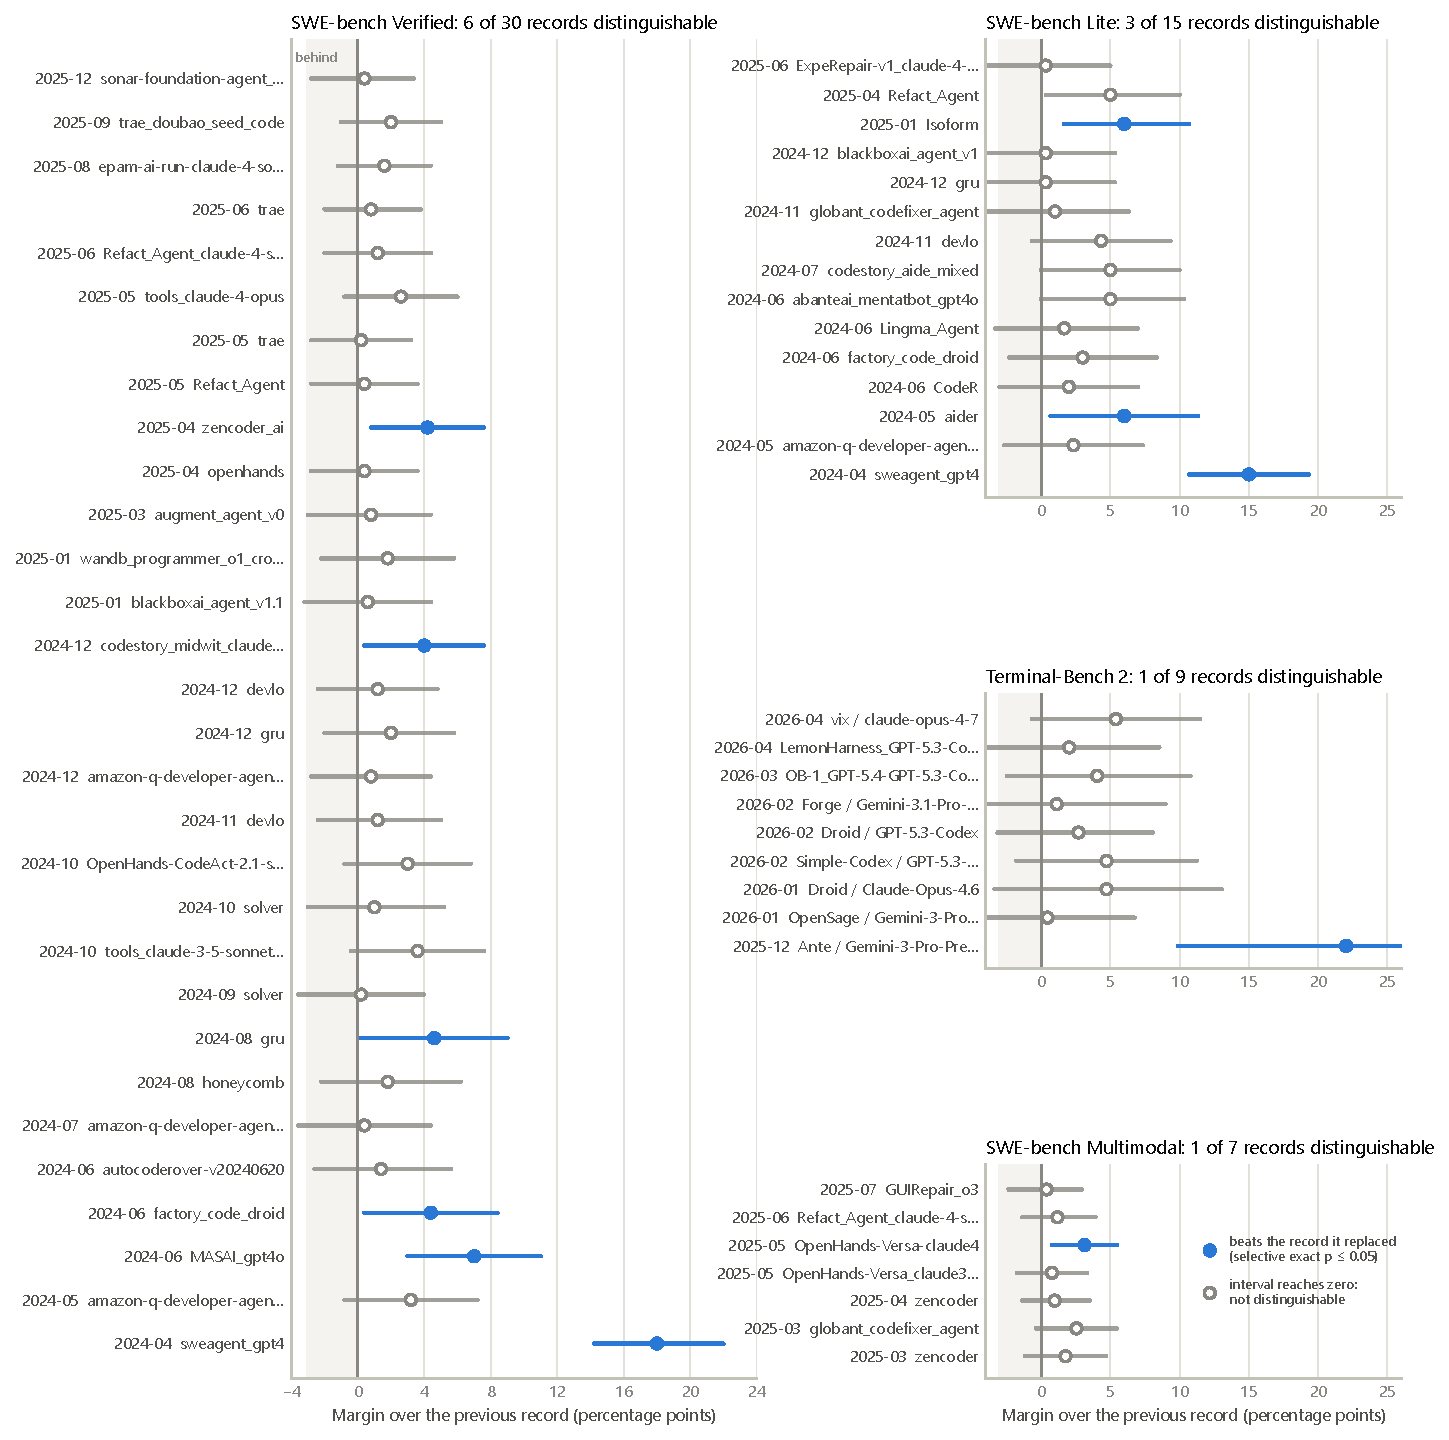
\includegraphics[width=\textwidth]{../figures/fig1_forest.pdf}
\caption{Every record step on four public leaderboards. Each row is a submission that set a new record; the dot is its margin over the record it replaced and the bar is the 95\% paired-bootstrap interval. Blue: the record can be told apart from the one before it (selective exact paired test, $p\le 0.05$). Gray: it cannot. Newest at the top. SWE-bench Test (\NumTestSig{} of \NumTestSteps{} steps significant) and Multilingual (no record steps under the primary ordering) are not shown.}
\label{fig:forest}
\end{figure}

\paragraph{Relation to earlier work.}
Statistical care in evaluation is not new: error bars for language-model evaluations~\citep{miller2024errorbars,madaan2024variance,bowyer2025clt,heineman2025signal}, power analysis for benchmark comparisons~\citep{card2020power}, cost-aware agent comparisons~\citep{kapoor2024agents}, run-to-run intervals for coding agents~\citep{huang2026deepswe}, the effect of the harness around a model~\citep{zhang2026harness,vats2026scaffold,arjmandi2026harness}, and degradation tests between model versions~\citep{kubler2026degradation}.
Three recent papers are close to ours.
\citet{liu2026converged} apply exact McNemar tests to adjacent pairs on four SWE-bench leaderboards, find that no adjacent pair in the Verified top 30 is separable, and estimate the number of instances a separation would need; our audit of time-ordered record steps, the repository-level test, Terminal-Bench, the confidence set, the winner's-curse correction and the tool are the additions.
\citet{kotawala2026resolution} give resolution diagnostics (minimum detectable effect, required sample size) for paired LLM evaluations, which our resolution section applies to agent boards.
\citet{jain2026lottery} argues, with simulations calibrated to LLM leaderboards, that the top-ranked model is the true best only a fraction of the time, and builds confidence sets of plausible winners with a paired-bootstrap multiple-comparisons-with-the-best procedure and a Holm step-down; it names models arriving over time as future work, which is our setting.
Sequential and online multiple testing, alpha-investing~\citep{foster2008alphainvesting}, online false-discovery-rate rules~\citep{javanmard2018online,ramdas2017lord}, online family-wise error control~\citep{tian2021onlinefwer} and the Ladder mechanism for leaderboards~\citep{blum2015ladder}, supply the level rules we use for records that arrive over time; what is new here is the per-step selective $p$-value for a record and the proof that the rules keep their guarantee when the hypotheses themselves are chosen by the record chain.
Rank intervals for leaderboards are developed by \citet{neuhof2026rankintervals,neuhof2026ranking}, with roots in \citet{mogstad2024ranks} and \citet{hung2019rank}; confidence sets for the best model in \citet{hansen2011mcs} and \citet{kim2025confidence}; Chatbot Arena reports bootstrap intervals and rank sets~\citep{chiang2024arena,chatzi2024ppr}.
On the winner's curse, \citet{andrews2024winners}, \citet{zrnic2025flexible}, \citet{petrouzeniou2024ranking} and \citet{hoff2025selective} give non-randomised corrections for a selection that has already been made, and \citet{bakshi2026winners} a randomised one; we use the polyhedral conditional method~\citep{lee2016exact,fithian2014optimal} and an iterated bootstrap~\citep{efron2011tweedie,efron2014model}, and run the hybrid of \citet{andrews2024winners} and the zoom interval of \citet{zrnic2025flexible} as baselines.
Inflation from hidden selection among privately tested variants~\citep{singh2025illusion,yang2026hidden} and benchmark overfitting~\citep{roelofs2019meta} are the sources of error this paper does not model.
An informal task-clustered bootstrap analysis of Terminal-Bench~2 reached a similar conclusion about its top two entries~\citep{lesswrong2026tbench}.

\paragraph{Contributions.}
This is an audit paper with a validated tool, and one methodological piece.
(i) The audit: every record step on six public agent leaderboards, tested with the selective exact test (the sign test conditional on the record event) and a repository-level test against each benchmark's resolution limit, with a split-half replication on the real data, a language-model leaderboard run through the same pipeline, and a bound on best-of-runs selection from the one board with repeated runs.
(ii) The methodological piece: a sequential certification procedure for record chains, a $p$-value valid under the record selection that we prove stays valid when the holder is itself a running maximum (Proposition~1), with two level rules, alpha-spending and online fallback, whose family-wise error control over the adaptively growing chain is proved without any independence assumption (Corollaries~1 and 2), the same guarantee for the procedure in which the leader moves only on certification (Corollary~3, through a monotonicity property of the $p$-value), and an online false-discovery-rate variant calibrated by simulation (Section~\ref{sec:methods}); to our knowledge this is the first certification procedure for leaderboard records with such a guarantee.
(iii) Rank intervals and a confidence set of the best system with a coverage study, and a selection-corrected score for the published winner, validated by simulation and by held-out tasks with Monte Carlo errors, against the hybrid of \citet{andrews2024winners} and the zoom interval of \citet{zrnic2025flexible}.
What is proved: the per-step test is exact under its null and stays valid for any holder chosen by an event increasing in its outcomes; the chain-wise error of three level rules is controlled for any dependence; everything else, including LORD++, the winner correction and the confidence set, rests on simulation and held-out data, and Table~\ref{tab:guarantees} in Section~\ref{sec:methods} says which is which.
(iv) \texttt{honestboard}, a dependency-light package with a command line and a check for new submissions,\footnote{Version 0.1.0, MIT licence: \url{https://github.com/jopoku16/honestboard}, with the built boards, every result file, the scripts behind each table and figure, and the manuscript source.} and reporting recommendations for benchmark maintainers.

\section{Setting}
A benchmark has $T$ tasks and $K$ systems.
System $k$ scores $y_{kt}\in[0,1]$ on task $t$: a pass or fail for single-run benchmarks, or the share of repeated trials that passed.
The reported score is $\hat p_k=T^{-1}\sum_t y_{kt}$.
The quantity of interest is $\theta_k=\E[y_{kt}]$, the expected score of system $k$ exactly as submitted, over the population of tasks that the benchmark's tasks are exchangeable draws from.
We treat tasks as the sampling unit.
All systems are scored on the same tasks, so the vector $\hat p=(\hat p_1,\dots,\hat p_K)$ is strongly correlated across systems and comparisons are paired.
Its covariance is estimated as $\hat\Sigma_{ij}=\{T(T-1)\}^{-1}\sum_t (y_{it}-\bar y_i)(y_{jt}-\bar y_j)$.
Where tasks come in clusters (repositories) we also use a cluster-sum version of this estimator and a cluster bootstrap.

\paragraph{Target of inference.}
Everything below is inference about $\theta_k$ in that sense: the score a system would have on further tasks of the same kind as the benchmark's (the same repositories, the same kinds of issues, the same scoring).
It is not inference about repositories the benchmark does not contain, about real deployments, or about a system after further tuning.
A reported score has three parts: $\theta_k$, noise from which tasks were drawn, and selection from development, because systems are tuned, and sometimes trained, with the public tasks in view~\citep{singh2025illusion,yang2026hidden}.
One run per system identifies only the second part.
Table~\ref{tab:scope} says which part each procedure addresses.
Development selection and run-to-run randomness of the agent are not modelled; both inflate reported scores, so the true overstatement of a winner may be larger than our correction removes.
Section~\ref{sec:audit} bounds one form of development selection, reporting the best of several runs, from the Terminal-Bench submissions that ran the whole benchmark more than once.

\begin{table}[h]
\centering\small
\begin{tabular}{p{4.6cm}p{5.4cm}p{4.6cm}}
\toprule
Source of error in a reported score & Addressed by & Status \\
\midrule
Which tasks were drawn & paired tests, rank intervals, confidence set, resolution, winner correction & modelled \\
Run-to-run randomness of the agent & nothing (single runs); quantified on Terminal-Bench from its five trials & not modelled \\
Development selection: variants tried, tuning and contamination on public tasks & nothing; best-of-runs reporting bounded from repeated runs on Terminal-Bench & not modelled \\
\bottomrule
\end{tabular}
\caption{What the procedures in this paper address.}
\label{tab:scope}
\end{table}

\section{Methods}\label{sec:methods}
\paragraph{Record test.}
Let $a$ be the record holder and $b$ a new submission with $\hat p_b>\hat p_a$.
With $n_b$ tasks solved only by $b$ and $n_a$ solved only by $a$, the exact paired test is the binomial (sign) test of $n_b$ among $n=n_a+n_b$ discordant tasks at probability one half, the exact form of McNemar's test~\citep{mcnemar1947}.
A record step is analysed \emph{because} $n_b>n_a$, so the test is run conditional on that event: with $X\sim\mathrm{Bin}(n,\tfrac12)$, the \emph{selective} $p$-value is
\[p_{\mathrm{sel}}=P(X\ge n_b\mid X>n/2)=\frac{P(X\ge n_b)}{P(X>n/2)}.\]
Under the task-wise null of the sign test (on each discordant task, $b$ is no likelier than $a$ to be the one that passes) and a fixed holder, $p_{\mathrm{sel}}$ is exactly super-uniform given the record event; Proposition~1 below extends that to a holder that is a running maximum.
For odd $n$ it equals the two-sided exact $p$-value.
For even $n$ it is larger, because $P(X>n/2)=\{1-P(X=n/2)\}/2<\tfrac12$, and the two-sided test then exceeds its level given the record event (with $n=44$ its conditional size is 5.5\%); a one-sided test at level $\alpha$ has size about $2\alpha$ among selected steps.
We call a step significant when $p_{\mathrm{sel}}\le0.05$; the two-sided and the one-sided test at 5\% are reported as sensitivities.
Section~\ref{sec:valid} checks the size by simulation under two nulls and by the step's position in the chain, and replicates the test on split halves of the real boards.
Holm's correction~\citep{holm1979} is applied over the record steps of one leaderboard.
For Terminal-Bench, where $y_{kt}$ is a rate, we use the sign-flip analogue, $P(S\ge s_{\mathrm{obs}}\mid S>0)$ for the sum $S$ of randomly signed per-task differences, with 20{,}000 draws; it is not exact.
Tasks from one repository are not independent, so the task-level test is the optimistic one and the repository-level test below the cautious one; Section~\ref{sec:valid} measures the difference.

\paragraph{Cluster-robust record test.}
For boards with repository labels we also run a repository-level sign-flip randomisation test: the per-task differences are summed within each repository and the repository sums are given random signs (all $2^G$ patterns when there are $G\le 14$ repositories).
Its selective form conditions on a positive sum in the same way.
It is valid if the repository sums are symmetric about zero under the null; with a dozen repositories it has little power, which is why the task-level count stays the headline and the repository-level count is reported beside it as the cautious one.

\paragraph{Same-date submissions.}
A record chain depends on the order of submissions with the same date.
The primary analysis orders them best first, which gives the fewest and largest steps, invents no intermediate record, and is the most generous reading for the leaderboard.
We also report worst first, which gives the most steps but can create records that were never on the leaderboard, so we treat it only as a bound.

\paragraph{Sequential certification of a record chain.}
A leaderboard decides about each record when it arrives, without knowing how many records will follow, so Holm over the realised chain is a retrospective device.
We give a procedure for the live setting.
For the $i$-th record step, with holder $a$ and challenger $b$, let $p_i=p_{\mathrm{sel}}$ be the selective $p$-value of the record test.
With a fixed holder it is super-uniform given that the step is a record, because the record event is exactly $\{X>n/2\}$.
A holder that is a running maximum has outcomes tilted upward, which makes $p_i$ conservative; this is a theorem, not only a simulation.

\begin{quote}
\textbf{Proposition 1.}
Let tasks be drawn independently, and let the \emph{conditional task-wise dominance null} hold: for each task, given the task and the outcomes of every other system, the probability that $b$ passes and $a$ fails is at most the probability that $a$ passes and $b$ fails.
(Equality is the null of the exact test, no task-level advantage for $b$; the null implies $\theta_b\le\theta_a$ but is not implied by it.)
Let $A$ be any event that, given the outcomes of every other system, is increasing in the outcomes of $a$ task by task; the event that $a$ holds the record among the earlier submissions, which depends on $a$ only through its total, is one.
Then, conditional on $A$, on the record event $\{n_b>n_a\}$, on the discordant set and on the outcomes outside it, $P(p_i\le u)\le u$ for every $u\in[0,1]$.
\end{quote}
\emph{Proof.}
Fix the discordant set $D$ with $|D|=n$, the outcomes of $a$ and $b$ outside $D$ and the outcomes of every other system.
Given these, the $n$ tasks of $D$ are independently $b$-only with probabilities at most one half, so the law of $n_b$ is dominated in the likelihood-ratio order by $\mathrm{Bin}(n,\tfrac12)$: Bernoulli laws are log-concave, and the likelihood-ratio order is preserved under convolution of log-concave laws~\citep[Section~1.C]{shaked2007stochastic}.
Within $D$, $a$ passes exactly the tasks that are not $b$-only, so $A$ is a decreasing event in the vector of $b$-only indicators, and by Efron's monotonicity theorem for independent variables with log-concave laws~\citep{efron1965polya}, $P(A\mid n_b=k,\dots)=g(k)$ is a decreasing function of $k$ (for the record event, an indicator of $\{k\le\text{constant}\}$).
Conditioning on $A$ multiplies the law of $n_b$ by $g$, which moves it downward in the likelihood-ratio order; conditioning further on $\{n_b>n/2\}$ restricts both laws to the same set and preserves the order.
Hence $n_b\mid A,\{n_b>n/2\}$ is stochastically at most $X\mid\{X>n/2\}$ with $X\sim\mathrm{Bin}(n,\tfrac12)$; $p_i$ is a decreasing function of $n_b$, so $P(p_i\le u)\le P\{p(X)\le u\mid X>n/2\}\le u$. $\square$

The proposition is checked by exhaustive enumeration on small boards in the package's tests, for holder events that are and are not functions of the total.
It also reaches the certified baseline, through a monotonicity property of the selective $p$-value.

\begin{quote}
\textbf{Lemma 1.}
$p_{\mathrm{sel}}$ decreases when a task won by the challenger is added to the discordant set and increases when a task won by the holder is added.
\end{quote}
The proof is a short Pascal-rule computation (Appendix~\ref{app:lemma}).
Whether $a$ was certified against its own reference, and whether no later submission has been certified against $a$, both depend on $a$'s outcomes only through counts of this kind, so by Lemma~1 the event ``$a$ is the certified holder when $b$ arrives'' is increasing in $a$'s outcomes given the other systems, and Proposition~1 applies to it.

The proposition covers both baselines: the leaderboard holder, which is a running maximum, and the certified holder, which was chosen by an earlier rejection.
Its null is the conditional task-wise dominance null, which is stronger than $\theta_b\le\theta_a$: when $b$ is a variant of an earlier system $c$, $b$ is likelier than $a$ to pass where $c$ passed, the per-task probabilities straddle one half, and the proof gives nothing, although every record may still be luck.
A rejection is therefore evidence against task-wise dominance of $a$ over $b$, the same reading as for McNemar's test; validity for the population-score null $\theta_b\le\theta_a$ alone is not proved, and Section~\ref{sec:valid} simulates the case where the two differ.
The level for the $i$-th record is set by one of three rules.
\emph{Alpha-spending:} $\alpha_i=6\alpha/(\pi^2 i^2)$, so that $\sum_i\alpha_i=\alpha$.
Its guarantee follows from Proposition~1 and a union bound, with no independence assumed.

\begin{quote}
\textbf{Corollary 1.}
Let the conditions of Proposition~1 hold for every pair that forms a record step on the leaderboard baseline, and let the $i$-th record step be tested at level $\alpha_i$ with $\sum_i\alpha_i\le\alpha$.
Then the probability that some record step at which the conditional task-wise dominance null holds is certified is at most $\alpha$, whatever the number of submissions, their order and the dependence between steps.
\end{quote}
\emph{Proof.}
Let $E_i(a,b)$ be the event that the $i$-th record step has holder $a$ and challenger $b$.
It is the intersection of the record event $\{n_b>n_a\}$ with an event that depends on the outcomes of $a$ only through its total score and is increasing in it: $a$ scored higher than every submission before it (and first within its date under the best-first ordering), no submission between $a$ and $b$ scored higher than $a$, and the number of record steps before $a$, which is determined by the submissions before $a$, is $i-1$.
Proposition~1 applies with $A$ that event, so $P(p_i\le\alpha_i\mid E_i(a,b),\ldots)\le\alpha_i$ whenever the null holds for $(a,b)$; summing over the disjoint events $E_i(a,b)$ gives $P(\text{a null pair is certified at step } i)\le\alpha_i$, and the union bound over $i$ gives the result. $\square$

Corollary~1 needs the level at step $i$ to be fixed by the conditioning, which holds for the leaderboard baseline because the record count before $a$ is determined by the submissions before $a$.
For the certified baseline the test count depends on how many submissions beat the certified holder, so test-indexed levels are not fixed in that sense; levels indexed by the holder's tenure are.

\begin{quote}
\textbf{Corollary 3.}
Under the conditions of Proposition~1 for every tested pair, the certified-baseline procedure has a super-uniform $p$-value at every test, and with the tenure-indexed levels $\alpha_{j,m}=\alpha\gamma_j\gamma_m$, where $j$ is one plus the number of certifications so far and $m$ the number of submissions since the certified holder arrived, it certifies some null pair with probability at most $\alpha$, for any dependence.
\end{quote}
\emph{Proof.}
Per-step validity is Proposition~1 with $A$ the certified-holder event, increasing by Lemma~1.
Given the conditioning of Proposition~1, $j$ is determined by the submissions before the holder together with the holder event, and $m$ by positions in the submission order, so the level is fixed; the levels used over any realised chain sum to at most $\alpha\sum_j\gamma_j\sum_m\gamma_m\le\alpha$, and the union bound of Corollary~1 applies. $\square$

The tenure-indexed rule spends budget on every submission since the holder arrived, tested or not, which costs power on long chains; the test-indexed spending and fallback levels on the certified baseline keep the per-step guarantee and are calibrated by simulation for the chain-wise one.

\emph{Online fallback:} $\alpha_i=6\alpha/(\pi^2i^2)+\alpha_{i-1}\,\mathbf 1\{\text{record } i-1\text{ was certified}\}$.
A certified record passes its level on to the next record, so a run of genuine records accumulates budget, as in the fixed-sequence fallback procedure~\citep{wiens2003fallback} and its online form~\citep{tian2021onlinefwer}; the rule dominates alpha-spending at every step and keeps the same guarantee.

\begin{quote}
\textbf{Corollary 2.}
Under the conditions of Corollary~1, the online fallback rule certifies some record step at which the conditional task-wise dominance null holds with probability at most $\alpha$.
\end{quote}
\emph{Proof.}
Let step $i$ be the first null step certified.
Every step in the run of consecutive certified steps ending at $i-1$ is then non-null, so the level used at $i$ is at most $L_i=\alpha\sum_{k\in R_i}\gamma_k$, with $\gamma_k=6/(\pi^2k^2)$ and $R_i$ the maximal run of non-null steps immediately before $i$ together with $i$ itself.
$R_i$ is determined by the identities of the earlier pairs, which are fixed by the conditioning of Proposition~1 on $E_i(a,b)$ and the earlier submissions, so Proposition~1 gives $P(\text{step } i\text{ is the first null step certified})\le\E[\mathbf 1\{\text{step } i\text{ is null}\}\,L_i]$.
The runs $R_i$ of distinct null steps are disjoint, so $\sum_{i\text{ null}}L_i\le\alpha\sum_k\gamma_k=\alpha$ on every realisation of the chain, and summing over $i$ gives the result. $\square$
\emph{LORD++}~\citep{ramdas2017lord}: an online false-discovery-rate rule with level $\alpha_i=\gamma_i W_0+(\alpha-W_0)\gamma_{i-\tau_1}+\alpha\sum_{j\ge2}\gamma_{i-\tau_j}$, where $\tau_j$ is the index of the $j$-th certified record, $W_0=\alpha/2$, and $\gamma_j$ is any sequence with $\sum_j\gamma_j\le1$; we use $\gamma_j=6/(\pi^2 j^2)$, the same sequence as the spending rule, because the sequence published with LORD++ is built for streams of thousands of tests and leaves almost no budget for a chain of thirty records.
Each certification earns back budget, so late records remain testable; LORD++ starts with half the spending rule's initial budget and overtakes it once records are certified.
Its guarantee is proved for independent $p$-values, and ours share tasks: alpha-spending and online fallback are the rules with the guarantee, and LORD++ is an alternative calibrated by simulation; \citet{javanmard2018online} give a more conservative variant for dependent $p$-values, which we have not implemented.
Two baselines are possible: test each leaderboard record against the record it replaced, or test every submission that beats the last \emph{certified} record against that record, so that the certified leader moves only when a record is certified, as in the Ladder~\citep{blum2015ladder}; Corollary~3 covers the second.
A normal-theory alternative that conditions on both selections at once (the polyhedral lemma applied to the event that $b$ is a record and $a$ was the holder) is described in Appendix~\ref{app:poly}; it needs a continuity correction on discrete scores and has no finite-sample guarantee, so it is reported only as a comparison.
Table~\ref{tab:guarantees} lists, for every procedure in the paper, what is proved and what rests on simulation.

\begin{table}[t]
\centering\small
\begin{tabular}{p{3.6cm}p{2.2cm}p{6.6cm}p{2.2cm}}
\toprule
Procedure & Baseline & Guarantee & Where \\
\midrule
Selective record test & either & exact size given the record event under the conditional task-wise dominance null; conservative when the holder is a running maximum or a certified holder & Prop.~1, Lemma~1 \\
Alpha-spending & leaderboard & family-wise error $\le\alpha$ over the chain, any dependence & Cor.~1 \\
Online fallback & leaderboard & the same, with a level never below spending's & Cor.~2 \\
Tenure-indexed spending & certified & family-wise error $\le\alpha$ over the chain, any dependence & Cor.~3 \\
Spending, fallback & certified & per-step validity proved; chain-wise rate by simulation & Prop.~1; Sec.~\ref{sec:valid} \\
LORD++ & either & false-discovery rate proved for independent $p$-values; dependent here, by simulation & Sec.~\ref{sec:valid} \\
Holm over the realised chain & leaderboard & retrospective, adaptive family; by simulation & Sec.~\ref{sec:valid} \\
Polyhedral $p$-value & leaderboard & none; continuity-corrected, by simulation & App.~\ref{app:poly} \\
Hybrid and zoom intervals & -- & coverage under normality with known covariance & Sec.~\ref{sec:methods} \\
Iterated bootstrap & -- & none; by simulation and held-out tasks & Sec.~\ref{sec:valid} \\
Confidence set of the best & -- & retains a truly best system at about the nominal rate; by simulation & Sec.~\ref{sec:valid} \\
\bottomrule
\end{tabular}
\caption{What is proved and what is simulated, for every procedure in the paper.}
\label{tab:guarantees}
\end{table}

\paragraph{Lag.}
For each record we find how many records back one must go before the record is significantly better than that earlier record (same test, no correction).
A lag of one means the record can be told apart from the one it replaced.

\paragraph{Resolution.}
Let $s$ be the median standard deviation of the per-task paired differences between neighbouring systems in the ranking of the ten highest-scoring systems.
With $z=\Phi^{-1}(0.975)+\Phi^{-1}(0.80)$, the paired test at level 0.05 (two-sided; the selective record test has the same critical value up to the even-$n$ correction) detects a true difference of $\mathrm{MDD}=z\,s/\sqrt{T}$ (the minimum detectable difference) with 80\% power, and resolving a difference $\Delta$ with that power takes $(zs/\Delta)^2$ tasks.
A task bootstrap of $s$ gives an interval for both numbers.
The smallest margin the test calls significant for a typical pair is about $1.96\,s/\sqrt{T}$, roughly 0.7 of the MDD.
This is a normal approximation~\citep{card2020power,kotawala2026resolution}; Section~\ref{sec:valid} checks it by simulation.

\paragraph{Rank intervals and top-rank frequency.}
We resample tasks with replacement, recompute all scores and ranks (tied systems share the better rank), and report the 2.5th and 97.5th percentiles of each system's rank.
The top-rank frequency of a system is the share of resamples in which it has the top score, with ties split equally.
It is a resampling frequency, not a posterior probability that the system is best.
Section~\ref{sec:valid} shows that the intervals cover the true rank when the true gaps are as large as the observed ones but not when leaders are truly tied, so the confidence set below is the statement to use about who could be best.

\paragraph{Confidence set of the best.}
Following multiple comparisons with the best~\citep{hsu1981mcb}, as adapted to paired bootstraps by \citet{jain2026lottery}, we keep every system that no rival beats by more than a simultaneous margin.
Let $\hat s_{ij}$ be the standard error of $\hat p_j-\hat p_i$ from $\hat\Sigma$ and $\hat p^*$ bootstrap scores.
For each system $i$ let $M_i=\max_{j\ne i}\{(\hat p_j^*-\hat p_i^*)-(\hat p_j-\hat p_i)\}/\hat s_{ij}$, the largest studentised deviation of any rival from $i$ in a resample.
System $i$ stays in the set if $\hat p_j-\hat p_i\le c\,\hat s_{ij}$ for all $j$, with $c$ the largest over $i$ of the $(1-\alpha)$ quantile of $M_i$.
A fixed truly best system is then retained with probability about $1-\alpha$, which is all the set promises; our earlier draft used the quantile of $\max_i M_i$, an all-pairs bound that gives larger sets, and we report both.
The guarantee is asymptotic and approximate, and in our simulations the set is conservative.
The set says who cannot be excluded, not who is likely to be best.

\paragraph{The winner's curse.}
Let $w=\arg\max_k\hat p_k$.
The reported $\hat p_w$ overstates $\theta_w$ on average because $w$ was selected for being large.
We consider two corrections.

\emph{Conditional (polyhedral) method.}
Treat $\hat p\sim N(\theta,\hat\Sigma)$ with $\hat\Sigma$ known.
The event that $w$ wins is $\{\hat p_j-\hat p_w\le 0,\ j\ne w\}$.
By the polyhedral lemma~\citep{lee2016exact,fithian2014optimal}, conditional on this event and on the part of $\hat p$ uncorrelated with $\hat p_w$, the winner's score is a normal distribution with mean $\theta_w$ and variance $\Sigma_{ww}$ truncated to an interval $[V^-,V^+]$ whose limits depend only on the other systems' scores and on $\hat\Sigma$.
Inverting the truncated-normal distribution function gives a median-unbiased estimate and a confidence interval for $\theta_w$ that are valid after selection.
It is exact under normality but undefined when the winner ties its runner-up, and nearly so when the margin is small, because then the observed score sits at the edge of the truncation region and the interval is unbounded; two of our six real boards have an exact tie at the top.

\emph{Baselines.}
Two published corrections run alongside.
The hybrid of \citet{andrews2024winners} conditions the polyhedral distribution further on the event that $\theta_w$ lies in a level $1-\beta$ projection interval, simultaneous over all systems; that bounds the truncation set, so the interval is never unbounded and stays inside the projection interval, and the conditional level is adjusted to $(\alpha-\beta)/(1-\beta)$ so that unconditional coverage is at least $1-\alpha$. Its estimate is median-unbiased under the hybrid distribution. We use $\beta=\alpha/10$.
The zoom correction of \citet{zrnic2025flexible}, in its simplest, locally simultaneous form~\citep{zrnic2024locally}, spends a share $\nu$ of the error budget on level $1-\nu$ simultaneous intervals for every system, keeps the plausible winners (the systems whose upper limit reaches the largest lower limit), and spends the remaining $\alpha-\nu$ on a simultaneous interval over that set alone; it corrects the interval, not the point estimate, and we use $\nu=\alpha/10$.
Both are exact under normality with known covariance; the simultaneous quantiles are computed by Monte Carlo from $\hat\Sigma$.
\citet{hoff2025selective} is not implemented.

\emph{Iterated bootstrap.}
In the bootstrap world the true scores are the observed scores, so the selection bias can be measured.
Draw a task resample, let $w^*$ be its winner, and set $\Delta^*=\hat p^*_{w^*}-\hat p_{w^*}$.
The plug-in correction is $\hat p_w-\hat b_1$ with $\hat b_1=\E^*\Delta^*$~\citep{efron1993bootstrap,efron2014model}.
It leaves bias because the observed scores of the leaders are more spread out than their true scores, so selection is less severe in the bootstrap world than in reality.
A second bootstrap level estimates the bias that remains: $\hat\theta_w=\hat p_w-2\hat b_1+\E^*\hat b_1^*$, where $\hat b_1^*$ is the plug-in bias computed from each outer resample.
The interval is $\hat\theta_w$ minus the quantiles of the centred $\Delta^*$.
It is defined for ties and works with cluster resampling.
Neither correction comes with a general theory here: the conditional method is exact only under normality with known covariance, and the iterated bootstrap is justified by its performance in Section~\ref{sec:valid}, not by a consistency result; the maximum is a non-smooth functional, so bootstrap consistency is not guaranteed near ties.

\section{Data}\label{sec:data}
We use per-task results published by the leaderboards themselves.
For SWE-bench~\citep{jimenez2024swebench,openai2024verified,yang2024swebenchmm,swebenchmultilingual} we use the submission records in the public \texttt{experiments} repository~\citep{swebenchexperiments}: lists of resolved task identifiers per submission, with the official task lists from the dataset listings, so tasks nobody solved are counted.
Verified has \NumVerifiedK{} usable submissions out of \NumMissingFound{} on 500 tasks; Lite has \NumLiteK{} on 300, Test \NumTestK{} on \NumTestT{}, Multimodal \NumMultimodalK{} on \NumMultimodalT{}, and Multilingual \NumMultilingualK{} on \NumMultilingualT{}.
Each submission is one run, dated by the date in its folder name; 11 of the 14 Multilingual submissions share one date, so its record chain depends on the ordering rule and has no steps under the primary rule.
Two Verified submissions tie exactly for first (396 of 500 tasks, differing on 36 tasks), and two Multimodal submissions tie for first; we name both and report the one with the higher top-rank frequency as the leader.

The \NumMissingN{} Verified submissions without a per-task file are dated \NumMissingFrom{} to \NumMissingTo{} and report an aggregate score in their metadata.
Their median is \NumMissingMedian\% against \NumIncludedMedian\% for the included submissions, so they are not a random subset.
Their highest score is \NumMissingMax\%, below the record of \NumIncludedMax\%, and by aggregate score none would have been a record holder: the chain built from all \NumMissingFound{} submissions has the same \NumVerifiedSteps{} steps.
They cannot have been the predecessor of a record we tested, but they are absent from the ranks, the confidence set and the winner's selection pool, and their per-task outcomes are unknown.

For Terminal-Bench~2~\citep{merrill2026terminalbench,terminalbench2026} we use the job-level result files in the leaderboard dataset.
Every trial named in a file is counted once: trials listed with reward 1 pass, trials listed with reward 0 fail, and trials that appear only in the error lists (agent errors, timeouts) count as failures.
The per-task score is the share of that task's trials that passed.
Of \NumTBFound{} submissions, \NumTBDroppedNoResults{} whose job files hold no per-task results, \NumTBDroppedVersion{} with a job labelled as benchmark version 2.1 and \NumTBDroppedMissing{} with missing tasks or dates are dropped, leaving \NumTBK{} on \NumTBTasks{} tasks.
The leaderboard nominally runs five trials per task, but \NumTBPooled{} submissions pool several jobs, and across kept submissions the number of trials on a task ranges from \NumTBTrialsMin{} to \NumTBTrialsMax{}; \NumTBExactlyFive{} submissions have exactly five everywhere.
Most job files do not name a benchmark version; we take the dataset's path (the 2.0 leaderboard) at its word.

For the non-agent comparison we use LiveBench~\citep{white2025livebench}, a leaderboard of language models with objective per-question scoring, from the per-question judgments file the leaderboard is computed from (the \texttt{livebench/model\_judgment} dataset, April 2025 version: \NumLBModelsFile{} models and \NumLBQuestionsFile{} questions in three categories, coding, instruction following and language).
Its questions rotate, so models were judged on different sets; we keep the \NumLBQuestionsKept{} questions present for at least half of the models and the \NumLBModelsKept{} models that have every one of them (\NumLBModelsDropped{} dropped, most of them partial re-judgings), average the \NumLBRepeated{} repeated judgments of one model on one question, and date a model by its earliest judgment in the file, from \NumLBFirstDate{} to \NumLBLastDate{}; \NumLBOnFirstDate{} models share the first date.
Scores are credit in $[0,1]$, \NumLBShareBinary\% of them 0 or 1, and the clusters are its \NumLBNTasks{} tasks.
The data and code to rebuild every board are in the project repository.

\section{Validation}\label{sec:valid}
\subsection{Is the record test calibrated?}
We simulate from a model fitted to SWE-bench Verified: per-task difficulties are the fitted logits of the mean pass rate of the 30 strongest systems (standard deviation \NumSimSdLogit{} on the logit scale), a system passes task $t$ with probability $\mathrm{sigmoid}(a_k+L_t)$, and the outcomes of different systems on a task are linked by a Gaussian copula with correlation $\rho=\NumSimRho$, tuned so that the paired spread between two equally able systems (\NumSimSdSim) matches the real board (\NumSimSdReal); real systems share base models and harnesses, so they agree on far more tasks than shared difficulty alone would give.
Two nulls are simulated (Table~\ref{tab:recordtest}).
In the \emph{global null}, \NumSimK{} equally able systems arrive in sequence, so every record is luck and the holder is a running maximum (\NumNullR{} boards per size).
In the \emph{selected-step null}, holder and challenger are equally able and the holder is not inflated; we keep the pairs in which the challenger scored higher (\NumNullSelPairs{} pairs per size), which is the record condition.
At 500 tasks the one-sided test at 5\% rejects \NumNullSelOneB\% of selected steps, close to the $2\alpha$ predicted above, the two-sided test \NumNullSelTwoB\% and the selective test \NumNullSelSelB\%.
Under the global null the selective rate is \NumNullSelectiveB\% averaged over the chain, but the average hides the position: the first step of a chain, where the holder is the first submission, conditioned only on no earlier record and so mildly inflated, rejects \NumNullPosFirstOneB\% one-sided and \NumNullPosFirstSelB\% selective, and later steps against an inflated holder almost never (Table~\ref{tab:position}).
The selective test is at or below 5\% given the record event by construction, and the simulation agrees in every case, also with the model fitted to Lite, Terminal-Bench and LiveBench (Appendix~\ref{app:otherboards}); the two-sided test differs from it only through the even-$n$ effect, and the one-sided test does not hold its level.
The chance that Holm rejects at least one step on a global-null board is \NumNullHolmB\%.
A second simulation checks the resolution formula: at the formula's minimum detectable difference the simulated power of the selective test is \NumPowerAtMddSelB{} at 500 tasks (Table~\ref{tab:power}), against a target of 0.80.

A split-half check on the real boards asks whether the test separates genuine records from lucky ones (Table~\ref{tab:split}).
For every record step and \NumSplitR{} random halves of the tasks, the test is run on one half and the challenger's margin over the holder on the other half is recorded.
Steps significant on the first half (\NumSplitSigShare\% of splits, against \NumSplitNullSigShare\% under the null reference below) have a positive margin on the second in \NumSplitSigRep{} of cases and a significant one in \NumSplitSigRepSig{}, against \NumSplitNonRep{} and \NumSplitNonRepSig{} for the rest.
Every step is a record on the full data, so the two halves are negatively dependent given the full margin and even a lucky record replicates more often than not; a null reference simulated for each step with its own number of discordant tasks (fair-coin signs conditioned on the full-data record event, then the same split) gives \NumSplitNullSigRep{} for significant and \NumSplitNullNonRep{} for non-significant first halves.
Significant steps replicate far above that reference and non-significant steps at about it, on every board, which is what a test that separates genuine records from lucky ones should produce; the pooled figures are dominated by SWE-bench Test, and Multimodal and Terminal-Bench contribute few significant splits.

\begin{table}[t]
\centering\small
\resizebox{\textwidth}{!}{\begin{tabular}{lrrrrrrr}
\toprule
 & & \multicolumn{3}{c}{Half 1 significant} & \multicolumn{3}{c}{Half 1 not significant} \\
Board & Steps & share of splits & replicates & null reference & share of splits & replicates & null reference \\
\midrule
SWE-bench Verified & 30 & 10\% & 0.85 & 0.48 & 90\% & 0.76 & 0.74 \\
SWE-bench Lite & 15 & 13\% & 0.87 & 0.45 & 87\% & 0.78 & 0.73 \\
SWE-bench Test & 13 & 63\% & 0.99 & 0.49 & 37\% & 0.88 & 0.75 \\
SWE-bench Multimodal & 7 & 5\% & 0.71 & 0.47 & 95\% & 0.80 & 0.73 \\
Terminal-Bench 2 & 9 & 10\% & 0.78 & 0.43 & 90\% & 0.80 & 0.73 \\
All boards & 74 & 19\% & 0.92 & 0.47 & 81\% & 0.79 & 0.74 \\
\bottomrule
\end{tabular}
}
\caption{Split-half replication of the record test on the real boards, \NumSplitR{} random halves per record step. Share of splits: how often the test on half 1 is significant. Replicates: share of those splits in which the challenger's margin on half 2 is positive. Null reference: the same quantity simulated for each step with its own number of discordant tasks under fair-coin signs conditioned on the full-data record event.}
\label{tab:split}
\end{table}

Tasks from one repository move together, and the task-level test treats them as independent.
Table~\ref{tab:clustersim} simulates the selected-step null with system-by-repository random effects on Verified's own \NumClusterG{} repositories, one of which holds 231 of the 500 tasks: each system's logit is shifted by $u_{kg}\sim N(0,\tau^2)$ in repository $g$, on top of the shared difficulty and the copula.
At $\tau=0.25$ the task-level selective test rejects \NumClusterTaskQuarter\% of null record steps and at $\tau=0.5$ \NumClusterTaskHalf\%, while the repository-level test stays at \NumClusterCluQuarter\% and \NumClusterCluHalf\%.
The data do not pin $\tau$ down.
A moment estimate from the per-repository residuals of the 30 strongest systems is zero, but the median ratio of the cluster-robust to the task-level standard error for neighbouring top-10 pairs on the real board is \NumClusterRealSe{}, against \NumClusterSeZero{} under independence with these repository sizes (the cluster-robust estimator is biased low when one repository dominates) and \NumClusterSeQuarter{} and \NumClusterSeHalf{} at $\tau=0.25$ and $0.5$, which points to a $\tau$ in that range.
The task-level counts are therefore optimistic where repositories matter, by an amount the data leave uncertain, and the repository-level counts in Section~\ref{sec:audit} are the cautious ones.

Tuning against the public tasks is outside the model, but its simplest form can be priced (Table~\ref{tab:tries}).
Let a team try $V$ equally able variants on the benchmark and submit the best; the record test conditions on one challenger having scored higher, not on the best of $V$, so under the selected-step null it rejects \NumTriesSizeTwo\% of record steps at $V=2$, \NumTriesSizeFive\% at $V=5$ and \NumTriesSizeTen\% at $V=10$, and the share of submissions that set a record rises from \NumTriesRecOne\% to \NumTriesRecTen\%.
If $V$ is declared, the Bonferroni-corrected $p$-value $\min(1,Vp_{\mathrm{sel}})$ holds the level (\NumTriesCorrFive\% at $V=5$, \NumTriesCorrTen\% at $V=10$); an exact test for the best of $V$ would need the per-task results of all $V$ variants, which a leaderboard does not see, so with $V$ alone declared the Bonferroni correction is what is available.
On a chain in which every submission is the best of $V$, the holder is inflated in the same way and the family-wise error falls to \NumTriesFwerTen\% at $V=10$; the danger is one team trying many variants against a holder that did not.
This is why the reporting checklist asks for the number of variants tried: without it the level of the record test is unknown.

\begin{table}[t]
\centering\small
\begin{tabular}{rrrrrr}
\toprule
 & \multicolumn{3}{c}{Selected-step null} & \multicolumn{2}{c}{Global null, chain of 40} \\
$V$ & sets a record & size, selective & size, $V$-corrected & FWER, selective & FWER, $V$-corrected \\
\midrule
1 & 48\% & 3.5\% & 3.5\% & 2.5\% & 2.5\% \\
2 & 64\% & 4.9\% & 2.5\% & 1.0\% & 0.0\% \\
3 & 73\% & 6.7\% & 2.1\% & 0.0\% & 0.0\% \\
5 & 81\% & 8.2\% & 1.8\% & 0.0\% & 0.0\% \\
10 & 90\% & 12.4\% & 1.5\% & 0.0\% & 0.0\% \\
\bottomrule
\end{tabular}

\caption{The record test when the submission is the best of $V$ equally able private tries on the same tasks (fitted Verified model, 500 tasks). Selected-step null: share of submissions that set a record, and the size of the selective test and of the $V$-corrected test among them. Global null: false certifications per board on 40-submission chains in which every submission is the best of $V$.}
\label{tab:tries}
\end{table}

\begin{table}[t]
\centering\small
\begin{tabular}{rrrr}
\toprule
$\tau$ (logit) & Task-level selective test & Repository-level test & SE ratio, repository / task \\
\midrule
0.00 & 3.8\% & 2.5\% & 0.88 \\
0.25 & 9.6\% & 3.1\% & 1.01 \\
0.50 & 24.9\% & 3.4\% & 1.32 \\
1.00 & 49.4\% & 3.7\% & 2.08 \\
\bottomrule
\end{tabular}

\caption{Size of the record test under system-by-repository random effects ($\tau$ on the logit scale): selected-step null on Verified's repositories, \NumClusterPairs{} pairs per level. SE ratio: mean ratio of the cluster-robust to the task-level standard error of the paired difference; the real board's median for neighbouring top-10 pairs is \NumClusterRealSe.}
\label{tab:clustersim}
\end{table}

\begin{table}[t]
\centering\small
\resizebox{\textwidth}{!}{\begin{tabular}{lrrrrrrrrrr}
\toprule
 & & & \multicolumn{3}{c}{Global null (holder is the best so far)} & \multicolumn{3}{c}{Selected-step null (holder not inflated)} & & \\
Fitted board & Tasks & Steps per board & selective & two-sided & one-sided & selective & two-sided & one-sided & Holm, any (selective) & Power at MDD \\
\midrule
SWE-bench Verified & 300 & 2.8 & 0.3\% & 0.3\% & 1.4\% & 3.7\% & 3.8\% & 8.2\% & 0.7\% & 0.77 \\
 & 500 & 2.8 & 0.5\% & 0.5\% & 1.7\% & 3.7\% & 3.9\% & 8.0\% & 0.7\% & 0.78 \\
 & 2,000 & 3.0 & 0.8\% & 0.8\% & 2.0\% & 4.4\% & 4.5\% & 9.1\% & 0.7\% & 0.77 \\
\addlinespace
SWE-bench Lite & 300 & 2.9 & 0.5\% & 0.5\% & 1.3\% & 3.9\% & 4.0\% & 8.1\% & 0.5\% & 0.76 \\
 & 500 & 3.0 & 0.8\% & 0.8\% & 2.1\% & 4.1\% & 4.3\% & 8.3\% & 1.3\% & 0.77 \\
 & 2,000 & 3.2 & 0.9\% & 0.9\% & 1.8\% & 4.1\% & 4.2\% & 9.2\% & 1.0\% & 0.78 \\
\addlinespace
Terminal-Bench 2 & 300 & 2.6 & 0.9\% & 1.0\% & 1.8\% & 3.1\% & 3.4\% & 7.1\% & 1.8\% & 0.74 \\
 & 500 & 2.8 & 0.4\% & 0.5\% & 1.7\% & 3.3\% & 3.3\% & 7.5\% & 0.8\% & 0.75 \\
 & 2,000 & 3.0 & 0.7\% & 0.8\% & 1.9\% & 4.1\% & 4.2\% & 8.5\% & 1.7\% & 0.78 \\
\addlinespace
LiveBench & 300 & 2.8 & 1.0\% & 1.1\% & 2.2\% & 3.5\% & 3.7\% & 7.9\% & 2.0\% & 0.77 \\
 & 500 & 2.9 & 0.7\% & 0.8\% & 2.2\% & 4.0\% & 4.3\% & 9.0\% & 0.8\% & 0.77 \\
 & 2,000 & 3.1 & 0.9\% & 1.0\% & 1.6\% & 4.4\% & 4.5\% & 9.0\% & 1.5\% & 0.77 \\
\bottomrule
\end{tabular}
}
\caption{Size of the record test among record steps, simulated from the fitted Verified model. Global null: \NumSimK{} equally able systems in sequence, rejection averaged over the chain. Selected-step null: equally able holder and challenger, challenger scored higher. A test with correct size rejects 5\% at the 5\% level.}
\label{tab:recordtest}
\end{table}

\subsection{Does the sequential certification hold its error rate?}
We simulate boards of \NumChainK{} submissions on \NumChainT{} tasks from the fitted model (\NumChainR{} boards per scenario; Table~\ref{tab:chainsim}).
Under the global null every record is luck.
In the staircase scenario the true score rises by \NumChainStep{} points every \NumChainPeriod{} submissions, so records are a mixture of genuine jumps and lucky steps within a level; in the late scenario one genuine jump of twice that size occurs halfway through the chain.
A certified step is false if the new system's true score does not exceed that of the system it was tested against.
Under the global null the unadjusted test certifies a false record on \NumChainNullUnadjFwer\% of boards, Holm over the realised chain on \NumChainNullHolmFwer\%, alpha-spending on \NumChainNullSpendFwer\%, online fallback on \NumChainNullFallFwer\%, LORD++ on \NumChainNullLordFwer\%, and the continuity-corrected polyhedral $p$-value under alpha-spending on \NumChainNullSpendPolyFwer\%; all hold the 5\% level.
With one late jump of twice the step size, the share of genuine records certified is \NumChainLateHolmPower\% for Holm, \NumChainLateSpendPower\% for alpha-spending, \NumChainLateFallPower\% for online fallback, \NumChainLateLordPower\% for LORD++ and \NumChainLateSpendPolyPower\% for the polyhedral $p$-value under alpha-spending, at false discovery rates of \NumChainLateHolmFdr\%, \NumChainLateSpendFdr\%, \NumChainLateFallFdr\%, \NumChainLateLordFdr\% and \NumChainLateSpendPolyFdr\%; the unadjusted test certifies \NumChainLateUnadjPower\% at a false discovery rate of \NumChainLateUnadjFdr\%.
The staircase's jumps of \NumChainStep{} points sit at the resolution limit of a \NumChainT{}-task board, and no rule with error control certifies more than \NumChainStairHolmPower\% of them (the unadjusted test certifies \NumChainStairUnadjPower\%); testing every submission above the last certified record instead of only leaderboard records raises the number of tests to \NumChainStairLordCertTests{} per board and the share certified to \NumChainStairLordCertPower\%, at a false discovery rate of \NumChainStairLordCertFdr\%.
Online fallback matches alpha-spending in every scenario here, where genuine records do not arrive in resolvable runs, and by construction never does worse; it pays off where consecutive records are genuine and resolvable, as on LiveBench below.
On the certified baseline, where every submission above the last certified record is tested, the tenure-indexed rule of Corollary~3 certifies a false record on \NumChainNullTenCertFwer\% of global-null boards and test-indexed alpha-spending on \NumChainNullSpendCertFwer\%; on the staircase they certify \NumChainStairTenCertPower\% and \NumChainStairSpendCertPower\% of genuine steps, and with one late jump \NumChainLateTenCertPower\% and \NumChainLateSpendCertPower\%, the price of spending budget on untested submissions.
In the variant scenario every submission is equally able, but \NumChainVariantShare\% of the submissions after the first are perturbations of a random earlier submission (its outcomes with passes flipped to failures at \NumChainVariantFlip\% and failures to passes at the rate that keeps the true score equal), the case in which the task-level null of Proposition~1 fails while every record is still luck: the unadjusted test certifies a false record on \NumChainVariantUnadjFwer\% of boards, Holm on \NumChainVariantHolmFwer\%, alpha-spending on \NumChainVariantSpendFwer\% and LORD++ on \NumChainVariantLordFwer\%, so the rules stay at or below their level there as well.
Alpha-spending has the stronger guarantee; LORD++ starts with half its initial budget and earns budget back on each certification, so it does worse when the only genuine record comes early and better on chains with several genuine jumps, as on the real boards below.

\begin{table}[t]
\centering\small
\resizebox{\textwidth}{!}{\begin{tabular}{lrrrrrrrrrr}
\toprule
 & \multicolumn{2}{c}{Global null} & \multicolumn{3}{c}{Staircase} & \multicolumn{3}{c}{One late jump} & \multicolumn{2}{c}{Variants, global null} \\
Procedure & FWER & certified & FDR & power & certified & FDR & power & certified & FWER & certified \\
\midrule
unadjusted, exact & 4.7\% & 0.05 & 5.4\% & 10\% & 0.7 & 5.7\% & 36\% & 0.42 & 4.0\% & 0.04 \\
Holm over the realised chain & 3.0\% & 0.03 & 0.0\% & 1\% & 0.1 & 0.3\% & 14\% & 0.14 & 1.0\% & 0.01 \\
alpha-spending, exact & 2.7\% & 0.03 & 0.3\% & 0\% & 0.0 & 1.3\% & 9\% & 0.10 & 1.3\% & 0.01 \\
online fallback, exact & 2.7\% & 0.03 & 0.3\% & 0\% & 0.0 & 1.3\% & 9\% & 0.10 & 1.3\% & 0.01 \\
LORD++, exact & 1.7\% & 0.02 & 0.0\% & 0\% & 0.0 & 1.0\% & 5\% & 0.06 & 0.0\% & 0.00 \\
alpha-spending, polyhedral & 3.3\% & 0.03 & 0.3\% & 1\% & 0.0 & 2.0\% & 12\% & 0.14 & 3.3\% & 0.03 \\
LORD++, polyhedral & 2.0\% & 0.02 & 0.0\% & 0\% & 0.0 & 1.0\% & 8\% & 0.09 & 0.0\% & 0.00 \\
LORD++, exact, certified baseline & 2.3\% & 0.02 & 0.1\% & 11\% & 2.7 & 1.0\% & 8\% & 0.71 & 0.7\% & 0.01 \\
\bottomrule
\end{tabular}
}
\caption{Sequential certification on simulated \NumChainK{}-submission boards of \NumChainT{} tasks (fitted Verified model). FWER: share of boards with at least one false certification. FDR: expected share of false certifications among certifications. Power: share of genuine record steps certified. Certified: mean number of certified records per board.}
\label{tab:chainsim}
\end{table}

\subsection{Does the winner's-curse correction work?}
We test the corrections on SWE-bench Verified, with Lite and Terminal-Bench as further checks.
\textbf{Known truth.} The observed score matrix is the population, a ``benchmark'' is $n$ tasks drawn with replacement, and each estimate is compared with the winner's true population score. This favours a bootstrap method, because the true gaps between systems equal the observed gaps.
\textbf{Equal leaders.} The hardest case: the top \NumBunchEqualTop{} systems are given the same true ability, outcomes are simulated from the fitted task-difficulty model, and the truth is known.
\textbf{Held-out tasks.} The real 500 tasks are split at random into a selection half and a validation half; the winner is chosen on the first and the estimate is compared with its score on the second, which is an unbiased but noisy stand-in for the truth.
\textbf{Held-out repositories.} The same with halves made of different repositories, chosen among the \NumVThreeSplits{} repository subsets that put 40 to 60\% of the tasks in the selection half (\NumVThreeSelMin{} to \NumVThreeSelMax{} tasks). The selection board keeps its repository labels and the corrections use cluster resampling. The validation score is adjusted by the mean difference in difficulty between the halves over all systems; the appendix reports the unadjusted target and the task-resampling corrections as well.
Alongside the two corrections we run the hybrid and zoom baselines of Section~\ref{sec:methods}.
Table~\ref{tab:valid} gives mean error with its Monte Carlo standard error, median error, root mean squared error, coverage and median length of the 95\% interval where the truth is known, how often each method is defined, and the mean and median error on the common subset of repetitions in which all six methods are defined, since the conditional and hybrid methods are undefined exactly where selection is most severe, at an exact tie for first.

\begin{table}[t]
\centering\scriptsize
\resizebox{\textwidth}{!}{\begin{tabular}{llrrrrrrrr}
\toprule
Setting & Estimator & Mean error (SE) & Median error & RMSE & Coverage & Length & Defined & Mean, common & Median, common \\
\midrule
Known truth, 500 tasks & reported & +0.92 (0.08) & +1.00 & 1.85 & 0.94 & 7.0 & 100\% & +0.95 & +1.00 \\
 & bootstrap & +0.08 (0.09) & +0.04 & 1.71 & 0.95 & 6.6 & 100\% & +0.12 & +0.07 \\
 & iterated bootstrap & $-$0.02 (0.09) & $-$0.11 & 1.77 & 0.94 & 6.6 & 100\% & +0.03 & $-$0.09 \\
 & conditional & +0.05 (0.11) & +0.23 & 2.10 & 0.98 & 9.4 & 90\% & +0.05 & +0.23 \\
 & hybrid (AKM) & +0.05 (0.11) & +0.23 & 2.10 & 0.98 & 9.5 & 90\% & +0.05 & +0.23 \\
 & zoom interval (ZF) & +0.92 (0.08) & +1.00 & 1.85 & 0.99 & 10.8 & 100\% & +0.95 & +1.00 \\
\addlinespace
Equal leaders, 500 tasks & reported & +2.19 (0.08) & +2.15 & 2.70 & 0.83 & 7.3 & 100\% & +2.23 & +2.35 \\
 & bootstrap & +0.65 (0.08) & +0.67 & 1.81 & 0.93 & 6.6 & 100\% & +0.70 & +0.71 \\
 & iterated bootstrap & +0.35 (0.09) & +0.32 & 1.80 & 0.93 & 6.6 & 100\% & +0.41 & +0.39 \\
 & conditional & +0.30 (0.14) & +0.57 & 2.60 & 0.97 & 15.0 & 86\% & +0.30 & +0.57 \\
 & hybrid (AKM) & +0.30 (0.14) & +0.57 & 2.60 & 0.97 & 10.6 & 86\% & +0.30 & +0.57 \\
 & zoom interval (ZF) & +2.19 (0.08) & +2.15 & 2.70 & 0.99 & 11.6 & 100\% & +2.23 & +2.35 \\
\addlinespace
Held-out tasks & reported & +2.04 (0.16) & +2.40 & 4.06 & -- & 9.9 & 100\% & +2.14 & +2.40 \\
 & bootstrap & +0.52 (0.16) & +0.63 & 3.68 & -- & 9.2 & 100\% & +0.66 & +0.65 \\
 & iterated bootstrap & +0.30 (0.17) & +0.41 & 3.71 & -- & 9.2 & 100\% & +0.45 & +0.42 \\
 & conditional & +0.72 (0.20) & +0.94 & 4.12 & -- & 15.7 & 82\% & +0.72 & +0.94 \\
 & hybrid (AKM) & +0.72 (0.20) & +0.94 & 4.12 & -- & 14.2 & 82\% & +0.72 & +0.94 \\
 & zoom interval (ZF) & +2.04 (0.16) & +2.40 & 4.06 & -- & 15.7 & 100\% & +2.14 & +2.40 \\
\addlinespace
Held-out repositories (cluster) & reported & +3.48 (0.17) & +2.98 & 5.21 & -- & 9.9 & 100\% & +3.90 & +3.70 \\
 & bootstrap & +1.81 (0.18) & +1.59 & 4.34 & -- & 15.6 & 100\% & +2.22 & +2.13 \\
 & iterated bootstrap & +1.85 (0.18) & +1.97 & 4.48 & -- & 15.6 & 100\% & +2.24 & +2.37 \\
 & conditional & +3.38 (0.24) & +3.71 & 5.90 & -- & 13.1 & 82\% & +3.38 & +3.71 \\
 & hybrid (AKM) & +3.43 (0.23) & +3.71 & 5.82 & -- & 12.2 & 82\% & +3.43 & +3.71 \\
 & zoom interval (ZF) & +3.48 (0.17) & +2.98 & 5.21 & -- & 13.5 & 100\% & +3.90 & +3.70 \\
\bottomrule
\end{tabular}
}
\caption{Winner's-curse correction on SWE-bench Verified, at least \NumValR{} repetitions per setting. Error is estimate minus target in percentage points; positive means overstated. Coverage is shown only where the truth is known; length is the median length of the 95\% interval in points. The zoom interval's point estimate is the reported score. The last two columns use the repetitions in which all six estimators are defined.}
\label{tab:valid}
\end{table}

\begin{figure}[t]
\centering
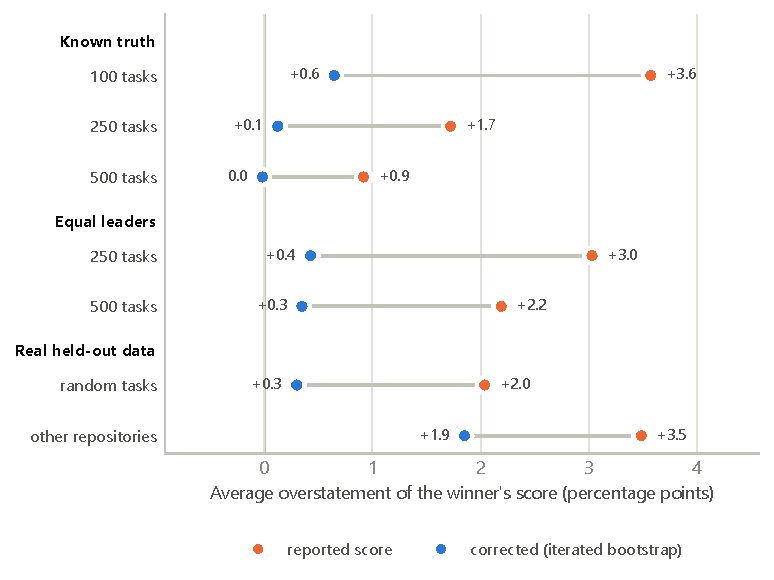
\includegraphics[width=0.88\textwidth]{../figures/fig4_winners_curse.pdf}
\caption{Average overstatement of the winner's score before and after the iterated bootstrap correction, on SWE-bench Verified. Orange: the reported score. Blue: the corrected score. The top two groups have known truth; the bottom group uses real held-out data, where the target is the winner's score on tasks not used for selection.}
\label{fig:bias}
\end{figure}

\paragraph{Results.}
In the known-truth runs the reported score of the winner overstates its true score by \NumVOneNCNaiveBias{} points at 500 tasks, \NumVOneNBNaiveBias{} at 250 and \NumVOneNANaiveBias{} at 100; with equally able leaders by \NumVBunchNCNaiveBias{} at 500 tasks and \NumVBunchNBNaiveBias{} at 250; and on real held-out tasks by \NumVTwoNaiveBias{} points.
The iterated bootstrap leaves \NumVOneNCIterBias{} points at 500 tasks (standard error \NumVOneNCIterSe), \NumVBunchNCIterBias{} with equal leaders and \NumVTwoIterBias{} on held-out tasks, removing about \NumVBunchNCReduction\% and \NumVTwoReduction\% of the overstatement in the last two cases; the plain bootstrap removes \NumVTwoReductionPlain\% on held-out tasks.
These percentages carry Monte Carlo errors of about $\pm$\NumVTwoReductionSe{} points, and the held-out repetitions are different splits of one board, so they are not independent.
Under a shift to other repositories the cluster-resampling iterated correction removes \NumVThreeReduction\%, so a benchmark whose tasks drift from the selection tasks will still overstate its winner.
The correction removes bias but does not make the winner's score more precise: on held-out tasks the root mean squared error of the iterated bootstrap (\NumVTwoIterRmse) is not below that of the plain bootstrap (\NumVTwoBootRmse), because most of the error in one system's score is sampling variance, not selection.
On the common subset the conditional method, which is median-unbiased by construction, has a median error of \NumVBunchNCCondMedC{} with equal leaders against \NumVBunchNCIterMedC{} for the iterated bootstrap, and it is defined in only \NumVBunchNCCondFin\% of those runs.
The hybrid interval is undefined only at an exact tie for first and is never unbounded: with equal leaders it covers in \NumVBunchNCHybCov{} of runs with a median length of \NumVBunchNCHybLen{} points, against \NumVBunchNCCondCov{} and \NumVBunchNCCondLen{} for the conditional interval, \NumVBunchNCIterCov{} and \NumVBunchNCIterLen{} for the iterated bootstrap, and \NumVBunchNCZoomCov{} and \NumVBunchNCZoomLen{} for the zoom interval, which leaves the point estimate uncorrected; the hybrid estimate's median error on the common subset is \NumVBunchNCHybMedC{} points.
The hybrid estimate coincides with the conditional one in every setting we ran, because the projection interval seldom binds at these sample sizes; its gain over the conditional method is the shorter interval, and on held-out tasks it leaves \NumVTwoHybBias{} points of overstatement against \NumVTwoIterBias{} for the iterated bootstrap.
The two baselines do not change the recommendation: the iterated bootstrap has the smallest bias among estimates that are defined at a tie, and the hybrid interval is the one to report when a guarantee under normality is wanted.
Coverage of the 95\% iterated interval in the known-truth runs rises from \NumVOneNANaiveCov{} for the reported score to \NumVOneNAIterCov{} at 100 tasks and is \NumVOneNCIterCov{} at 500 (\NumVOneNCNaiveCov{} for the reported score); it stays below nominal when tasks are few.
On Lite the iterated correction removes \NumLiteTwoReduction\% on held-out tasks but overshoots on held-out repositories (mean error \NumLiteThreeIterBias{} points against \NumLiteThreeNaiveBias{} for the reported score, with selection halves of only 120 to 180 tasks).
On Terminal-Bench (Appendix Table~\ref{tab:valtb}) the known-truth and equal-leaders results point the same way, but on real held-out halves of 44 tasks the iterated correction overshoots (mean error \NumTBTwoIterBias{} points against \NumTBTwoNaiveBias{} for the reported score), so the correction is not guaranteed to help on very small benchmarks.
On LiveBench (Appendix Table~\ref{tab:vallb}) equally able leaders overstate by \NumLBBunchNaiveBias{} points, of which the iterated bootstrap leaves \NumLBBunchIterBias{} and the hybrid \NumLBBunchHybBias{}; on held-out halves of its questions there is no overstatement to remove (\NumLBTwoNaiveBias{} for the reported score), because its leader is far ahead of the field, and the corrections leave it nearly untouched (\NumLBTwoIterBias{} and \NumLBTwoHybBias{}).

\subsection{Do the rank intervals and confidence sets cover?}
We use the known-truth setting again (\NumRankCovR{} repetitions; Table~\ref{tab:rankcov}).
The 95\% rank interval contains the true rank for \NumRankCovAllA{} (250 tasks) and \NumRankCovAllB{} (500 tasks) of the systems, for \NumRankCovTopA{} and \NumRankCovTopB{} of the ten truly best systems, and for \NumRankCovWinA{} and \NumRankCovWinB{} of the selected winners.
When the top \NumBunchEqualTop{} systems are equally able, the true rank of a leader is ill defined: under the convention that tied systems share rank 1 the interval covers it for only \NumRankBunchLeadA{} and \NumRankBunchLeadB{} of the leaders, under the average-rank convention for \NumRankBunchLeadAvgA{} and \NumRankBunchLeadAvgB{}, and it meets the block of tied ranks in \NumRankBunchBlockA{} and \NumRankBunchBlockB{} of cases.
The intervals describe the sampling variability of the rank statistic and should not be read as confidence intervals for a true rank when leaders are close~\citep{neuhof2026rankintervals,mogstad2024ranks}.
The confidence set behaves differently: in the same runs it contained each of the equally able leaders in \NumSetBunchInA{} (250 tasks) and \NumSetBunchInB{} (500 tasks) of repetitions, with sets of median size \NumSetBunchSizeA{} and \NumSetBunchSizeB{} against \NumBunchEqualTop{} tied systems, so it retains each tied leader at the nominal rate without being much larger than the tied block.
Table~\ref{tab:lottery} shows how often the observed winner is a truly best system in the known-truth runs: \NumVFourNCWin{} at 500 tasks, \NumVFourNBWin{} at 250 and \NumVFourNAWin{} at 100.

\begin{table}[t]
\centering\scriptsize
\resizebox{\textwidth}{!}{\begin{tabular}{lrrrrrrrrr}
\toprule
 & \multicolumn{3}{c}{Known truth: interval covers true rank} & \multicolumn{4}{c}{Equal leaders: interval covers} & \multicolumn{2}{c}{Equal leaders: confidence set} \\
Tasks & all & true top 10 & selected winner & rank 1 (min) & average rank & tied block & all & contains each leader & median size \\
\midrule
250 & 0.96 & 0.95 & 0.96 & 0.44 & 0.95 & 1.00 & 0.88 & 0.99 & 28 \\
500 & 0.96 & 0.96 & 0.97 & 0.42 & 0.95 & 1.00 & 0.88 & 0.99 & 23 \\
\bottomrule
\end{tabular}
}
\caption{Coverage of 95\% rank intervals and of the confidence set of the best, SWE-bench Verified, known-truth simulation. Equal leaders: the \NumBunchEqualTop{} top systems have equal true ability; the three conventions treat their true rank as 1, as the average of the tied ranks, or as the whole tied block.}
\label{tab:rankcov}
\end{table}


\section{Audit of six agent leaderboards, with a non-agent comparison}\label{sec:audit}
\begin{table}[t]
\centering\footnotesize
\resizebox{\textwidth}{!}{\begin{tabular}{lrrrrrrrrr}
\toprule
Board & Systems & Tasks & Top-rank freq. & 95\% set & Records sig. & Holm & Repository-level & MDD (pts) & Leader (\%): reported $\to$ adjusted \\
\midrule
SWE-bench Verified & 135 & 500 & 0.35 & 14 & 6/30 & 2 & 1/30 & 4.3 & 79.2 $\to$ 78.1 \\
SWE-bench Lite & 84 & 300 & 0.47 & 5 & 3/15 & 1 & 1/15 & 6.7 & 60.3 $\to$ 58.7 \\
SWE-bench Test & 24 & 2,294 & 1.00 & 1 & 9/13 & 9 & 7/13 & 2.2 & 52.6 $\to$ 52.6 \\
SWE-bench Multimodal & 12 & 510 & 0.38 & 5 & 1/7 & 0 & 1/7 & 3.8 & 36.5 $\to$ 35.3 \\
SWE-bench Multilingual & 14 & 300 & 0.54 & 9 & 0/0 & 0 & 0/0 & 7.2 & 72.7 $\to$ 71.2 \\
Terminal-Bench 2 & 67 & 89 & 0.80 & 10 & 1/9 & 1 & -- & 7.9 & 89.9 $\to$ 89.0 \\
\midrule
All boards & & & & & 20/74 & 13 & 10/65 & & \\
\bottomrule
\end{tabular}
}
\caption{Audit summary. Top-rank freq.: share of task resamples in which the leader has the top score. 95\% set: size of the confidence set of the best system. Records sig.: record steps that can be told apart from the previous record at the 5\% level (selective exact paired test, tasks as the sampling unit) over all record steps. Holm: significant after Holm correction within the board. Repository-level: the same count with repositories as the sampling unit, the cautious one. MDD: smallest difference detected with 80\% power. Last column: the leader's reported score and its task-sampling selection adjustment (iterated bootstrap); where two systems tie for first, the leader is the one with the higher top-rank frequency.}
\label{tab:audit}
\end{table}

\paragraph{Records.}
Only \NumTotalSig{} of \NumTotalSteps{} record steps (\NumTotalSigPct\%) are significant against the record they replaced by the selective test, and \NumTotalHolm{} (\NumTotalHolmPct\%) after Holm; the two-sided test finds the same \NumTotalTwoSided{} steps, and the one-sided test at 5\%, whose size among selected steps is about \NumNullSelOneB\% in simulation, finds \NumTotalOneSided{}.
The split by resolution is stark: \NumLargeSig{} of \NumLargeSteps{} on SWE-bench Test, \NumSmallSig{} of \NumSmallSteps{} on the five boards with at most 510 tasks.
Among the \NumSmallMarginSteps{} steps with a margin under two points, \NumSmallMarginSig{} reach significance.
Table~\ref{tab:sens} shows how the count moves with the choices we made: the repository-level test, the cautious one where tasks share repositories (Section~\ref{sec:valid}), leaves \NumClusterSig{} of the \NumClusterSteps{} SWE-bench steps against \NumSWEIidSig{} with the task-level test, and ordering same-date submissions worst first creates more steps (\NumWorstSteps{}) of which \NumWorstSigPct\% are significant, so the share of unresolved records barely changes.
A record that is not significant is not shown to equal its predecessor: for the non-significant records the 97.5\% upper bound of the margin has a median of \NumVerifiedUpperNonSig{} points on Verified (\NumLiteUpperNonSig{} on Lite, \NumTBUpperNonSig{} on Terminal-Bench), so improvements of that size are neither shown nor excluded.
These are single-run submissions.

\paragraph{Certified records.}
Run in time order, the sequential rules certify fewer records than the retrospective Holm count (Table~\ref{tab:chainaudit}): alpha-spending \NumCertTotalSpend{} and online fallback \NumCertTotalFall{}, the two rules with the proved guarantee, and LORD++, calibrated by simulation, \NumCertTotalLord{} of the \NumTotalSteps{} leaderboard records, against \NumCertTotalHolm{} for Holm and \NumCertTotalUnadj{} unadjusted; the polyhedral $p$-value, which also accounts for the holder's selection, gives \NumCertTotalLordPoly{} under LORD++.
On these chains no two consecutive records are both genuine and resolvable, so the fallback rule certifies the same \NumCertTotalFall{} records as spending; on LiveBench, where they are, it certifies all \NumLBSteps{} against \NumLBCertSpend{} for spending (Table~\ref{tab:nonagent}).
With 95\% confidence every record certified by either rule is genuine, so the six boards hold at least \NumCertTotalFall{} records that beat their predecessor task-wise.
With the certified baseline (Corollary~3), every submission that beats the last certified record is tested: the tenure-indexed rule, which carries the chain-wise guarantee, certifies \NumCertTotalTenCert{} of \NumCertTestsTenCert{} tested submissions across the boards, test-indexed alpha-spending \NumCertTotalSpendCert{} of \NumCertTestsSpendCert{}, and LORD++ \NumCertTotalLordCert{} of \NumCertTestsLordCert{}.
Figure~\ref{fig:certified} shows the leaderboard record line and the certified record line under the tenure-indexed rule on Verified and Lite: on Verified the certified leader moves \NumVerifiedCertTenCert{} times in \NumVerifiedK{} submissions, against \NumVerifiedSteps{} leaderboard records.

\begin{table}[t]
\centering\small
\resizebox{\textwidth}{!}{\begin{tabular}{lrrrrrrrr}
\toprule
Board & Records & Unadjusted & Holm & Spending & Fallback & LORD++ & LORD++ (polyhedral) & Spending (certified baseline) \\
\midrule
SWE-bench Verified & 30 & 6 & 2 & 2 & 2 & 2 & 2 & 7/56 \\
SWE-bench Lite & 15 & 3 & 1 & 1 & 1 & 1 & 1 & 4/31 \\
SWE-bench Test & 13 & 9 & 9 & 7 & 7 & 9 & 9 & 9/13 \\
SWE-bench Multimodal & 7 & 1 & 0 & 0 & 0 & 0 & 0 & 2/8 \\
SWE-bench Multilingual & 0 & 0 & 0 & 0 & 0 & 0 & 0 & 0/0 \\
Terminal-Bench 2 & 9 & 1 & 1 & 1 & 1 & 1 & 1 & 1/37 \\
\midrule
All boards & 74 & 20 & 13 & 11 & 11 & 13 & 13 & 23/145 \\
\bottomrule
\end{tabular}
}
\caption{Records certified by each rule, run in date order with the exact selective $p$-value unless noted. Unadjusted: selective exact test at 5\% per step. Holm: retrospective, over the realised chain. Spending and fallback (both with the proved chain-wise guarantee) and LORD++ (calibrated by simulation): sequential levels. Certified baseline: every submission that beats the last certified record is tested (shown as certified/tested); the tenure-indexed levels carry the chain-wise guarantee of Corollary~3, the test-indexed spending levels are calibrated by simulation.}
\label{tab:chainaudit}
\end{table}

\begin{figure}[t]
\centering
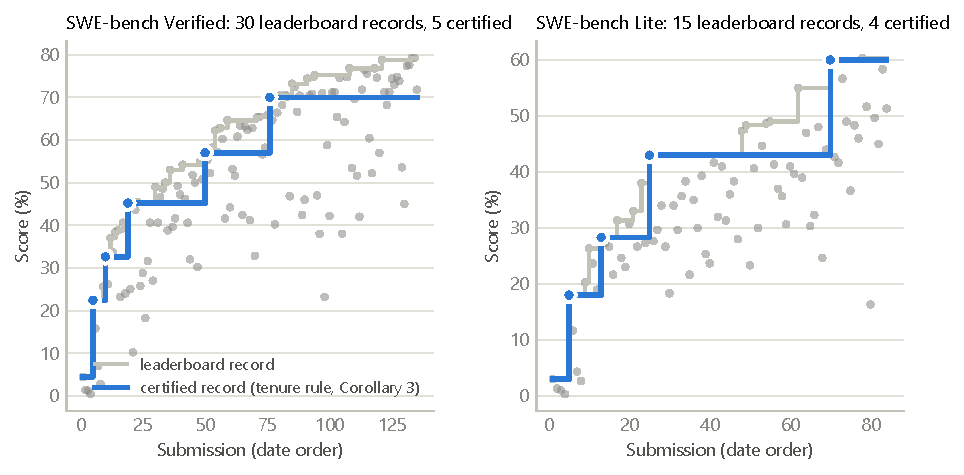
\includegraphics[width=\textwidth]{../figures/fig6_certified.pdf}
\caption{Leaderboard records and certified records in submission order. Gray dots: all submissions. Gray step: the leaderboard record. Blue step and dots: the certified record under the tenure-indexed rule of Corollary~3, which moves only when a submission is certified against the last certified record.}
\label{fig:certified}
\end{figure}

\begin{table}[t]
\centering\small
\resizebox{\textwidth}{!}{\begin{tabular}{lrrrrrr}
\toprule
Board & Steps & Selective (primary) & Two-sided & One-sided & Repository-level & Worst-first ordering \\
\midrule
SWE-bench Verified & 30 & 6 & 6 & 7 & 1 & 9/36 \\
SWE-bench Lite & 15 & 3 & 3 & 6 & 1 & 4/20 \\
SWE-bench Test & 13 & 9 & 9 & 10 & 7 & 13/17 \\
SWE-bench Multimodal & 7 & 1 & 1 & 1 & 1 & 1/7 \\
SWE-bench Multilingual & 0 & 0 & 0 & 0 & 0 & 1/10 \\
Terminal-Bench 2 & 9 & 1 & 1 & 1 & -- & 1/9 \\
\midrule
All boards & 74 & 20 & 20 & 25 & 10 (of 65) & 29/99 \\
\bottomrule
\end{tabular}
}
\caption{Number of record steps significant at the 5\% level under five choices: the primary selective exact test with best-first ordering of same-date submissions, the two-sided exact test, the one-sided test at 5\%, the repository-level sign-flip test (the cautious count), and worst-first ordering (more steps, shown as significant/steps).}
\label{tab:sens}
\end{table}

\paragraph{Resolution.}
Figure~\ref{fig:resolution} compares what each board can detect with the margins records are claimed by.
SWE-bench Verified detects differences of \NumVerifiedMDD{} points with 80\% power (task bootstrap 95\% interval \NumVerifiedMDDLo{} to \NumVerifiedMDDHi; \NumVerifiedMDDCluster{} with cluster-robust variance), calls a typical margin significant from about \NumVerifiedCritMargin{} points, and its median record margin is \NumVerifiedMedianMargin{}; resolving one point would take about \NumVerifiedTasksOnePt{} tasks (interval \NumVerifiedTasksOnePtLo{} to \NumVerifiedTasksOnePtHi) and two points about \NumVerifiedTasksTwoPt{}.
Lite detects \NumLiteMDD{} against a median margin of \NumLiteMedianMargin{}, Multimodal \NumMultimodalMDD{} against \NumMultimodalMedianMargin{}, Terminal-Bench~2 \NumTBMDD{} against \NumTBMedianMargin{} with 89 tasks, and SWE-bench Test \NumTestMDD{} against \NumTestMedianMargin{}, the one board whose typical record is above its resolution.
Table~\ref{tab:lags} gives how far back a record has to be compared before it is distinguishable.

\begin{figure}[t]
\centering
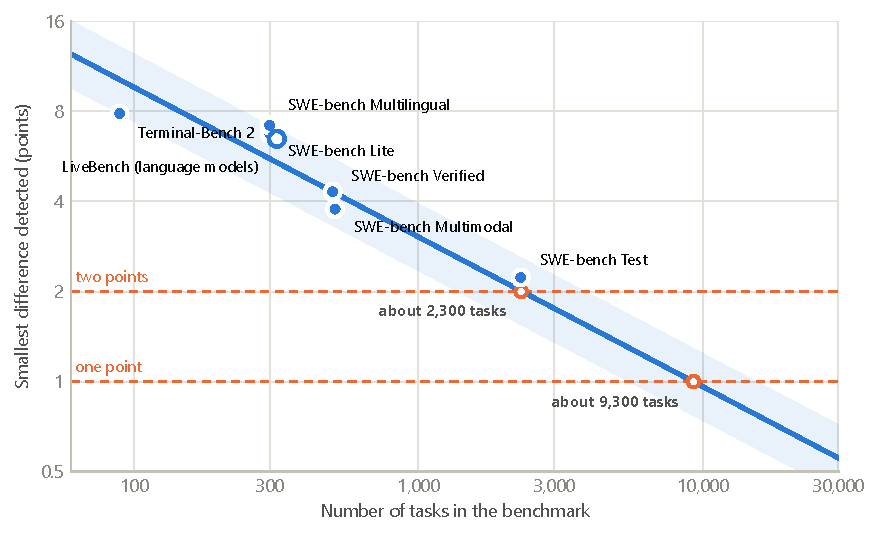
\includegraphics[width=0.92\textwidth]{../figures/fig2_resolution.pdf}
\caption{What a point costs. The smallest true difference a benchmark detects with 80\% power in the two-sided paired test at the 5\% level, against the number of tasks (both axes logarithmic). The line is SWE-bench Verified's paired spread and the band spans the boards; orange circles mark the number of tasks Verified would need to resolve one and two points. Filled dots are the six agent boards; the hollow dot is LiveBench, the language-model comparison.}
\label{fig:resolution}
\end{figure}

\begin{table}[t]
\centering\small
\resizebox{\textwidth}{!}{\begin{tabular}{lrrrr}
\toprule
Board & Median margin (pts) & Median lag & Beats previous record & Beats no earlier record \\
\midrule
SWE-bench Verified & 1.5 & 2 & 20\% & 0\% \\
SWE-bench Lite & 3.0 & 2 & 20\% & 0\% \\
SWE-bench Test & 3.3 & 1 & 69\% & 0\% \\
SWE-bench Multimodal & 1.2 & 2 & 14\% & 14\% \\
Terminal-Bench 2 & 4.0 & 3 & 11\% & 0\% \\
\bottomrule
\end{tabular}
}
\caption{Lag analysis. Median margin of a record; median number of records back needed before a record is significantly better than that earlier record (lag); the share of records that beat the one they replaced; and the share that beat no earlier record on the board.}
\label{tab:lags}
\end{table}

\paragraph{Ranks.}
Figure~\ref{fig:ranks} shows the leaders.
On Verified the two tied leaders rank first in \NumVerifiedPBest{} and \NumVerifiedPBestOther{} of task resamples, and the 95\% confidence set of the best system has \NumVerifiedSet{} systems (\NumVerifiedSetSim{} with the all-pairs bound; \NumVerifiedSetCluster{} when resampling repositories).
Terminal-Bench~2 shows the opposite case: the leader is first in \NumTBPBest{} of resamples, yet with 89 tasks the confidence set still has \NumTBSet{} systems, because systems far below the leader cannot be excluded at that sample size.
A clear leader and a long confidence set can both be true: the set retains each truly best system at about the nominal rate but cannot exclude systems far below the leader at that sample size, so its size overstates the number of plausible winners.

\begin{figure}[t]
\centering
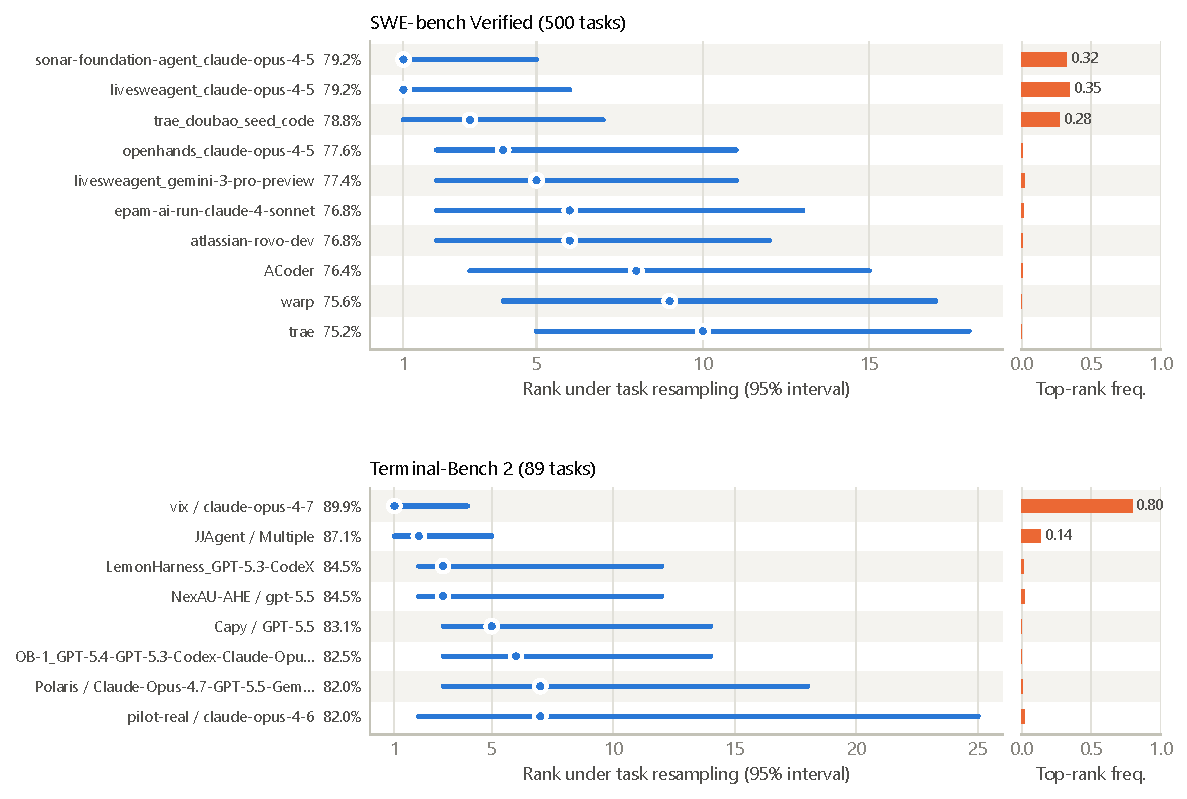
\includegraphics[width=0.92\textwidth]{../figures/fig3_rank_intervals.pdf}
\caption{Rank intervals (95\%, task resampling) for the leading systems. The dot is the observed rank and the reported score follows each name. Orange bars: share of resamples in which the system ranks first.}
\label{fig:ranks}
\end{figure}

\paragraph{Adjusted winners.}
The task-sampling selection adjustment of the leader's score, which covers luck in which tasks were drawn and nothing else, is in the last column of Table~\ref{tab:audit}.
On Verified the leader's reported \NumVerifiedWinnerObs\% becomes \NumVerifiedWinnerAdj\% (95\% interval \NumVerifiedWinnerCiLo{} to \NumVerifiedWinnerCiHi); on Lite \NumLiteWinnerObs\% becomes \NumLiteWinnerAdj\% (\NumLiteWinnerCiLo{} to \NumLiteWinnerCiHi).
On SWE-bench Test the adjustment is negligible because the leader is far ahead and the benchmark is large.
Tuning against public tasks is not covered, so the true overstatement may be larger.
The conditional method is undefined on Verified and Multimodal, where the top is an exact tie, and gives \NumLiteCondAdj\% on Lite and \NumTBCondAdj\% on Terminal-Bench.

\paragraph{Run randomness on Terminal-Bench.}
Terminal-Bench runs several trials per task, which lets us split the variance of a score into task sampling and run-to-run randomness.
For the 20 strongest systems, run randomness is a median \NumTBRunShareSingle\% (range \NumTBRunShareSingleMin{} to \NumTBRunShareSingleMax\%) of the per-task variance of a single-run score, and \NumTBRunShareFive\% of a five-trial score; for the paired difference between neighbouring top-10 systems it is \NumTBPairRunShareSingle\% single-run and \NumTBPairRunShareFive\% with five trials.
A single-run coding-agent score therefore carries run noise of the same order as task-sampling noise, which the SWE-bench boards, with one run per submission, cannot show.

\paragraph{Development selection, seen through repeated runs.}
Selection among privately tested variants cannot be measured from one run per system, but the Terminal-Bench submissions that ran the whole benchmark several times show the scale of its simplest form.
\NumTBJobSubs{} kept submissions have at least two complete jobs (median \NumTBJobMedianJobs); the between-job standard deviation of a submission's score has median \NumTBJobSd{} points (interquartile range \NumTBJobSdLo{} to \NumTBJobSdHi), and a team that had reported its best job instead of the mean of its jobs would have gained a median \NumTBJobInflMedian{} points (mean \NumTBJobInflMean, at most \NumTBJobInflMax).
Read, as an illustration of scale, as a model of development selection in which a team tries $V$ variants whose scores scatter like repeated runs and submits the best, the expected inflation is $\E[\max_{v\le V} Z_v]$ times that spread: \NumTBJobInflVTwo{} points for two variants, \NumTBJobInflVFive{} for five and \NumTBJobInflVTen{} for ten, of the same order as the winner's-curse bias from task sampling and as this board's median record margin (\NumTBJobInflVFive{} against \NumTBMedianMargin{} points).
The leaderboard reports the mean over jobs, so this is a bound on what best-of-runs reporting would add, not a finding that it happened, and selection among variants that differ by more than run noise can add more.

\paragraph{A non-agent comparison.}
The procedures are not specific to agents, and LiveBench shows what they return on a leaderboard of language models with objective per-question scoring (Table~\ref{tab:nonagent}).
With \NumLBT{} questions its resolution is as coarse as Lite's (minimum detectable difference \NumLBMDD{} points, about \NumLBTasksOnePt{} questions to resolve one point).
Its \NumLBSteps{} record steps under the primary ordering have a median margin of \NumLBMedianMargin{} points, above the board's critical margin of \NumLBCritMargin{}; \NumLBSig{} pass the unadjusted test, \NumLBHolm{} Holm, and the sequential rules certify \NumLBCertSpend{} (alpha-spending), \NumLBCertFall{} (online fallback, whose inherited budget carries a run of genuine records) and \NumLBCertLord{} (LORD++); under the worst-first ordering of the \NumLBOnFirstDate{} models that share the first date there are \NumLBWorstSteps{} steps, \NumLBWorstSig{} of them distinguishable.
Its leader ranks first in \NumLBPBest{} of resamples and is alone in the confidence set, so the selection correction leaves its score where it is (\NumLBWinnerObs\% to \NumLBWinnerAdj\%).
Four records are too few to support a contrast with the agent boards, and the board is a reconstruction (three of six categories, partial credit, models dated by their first judgment in a snapshot file); the comparison shows that the tools apply unchanged, and that on a board of the same resolution it is the size of the margins that moves the counts.

\begin{table}[t]
\centering\small
\resizebox{\textwidth}{!}{\begin{tabular}{lrrr}
\toprule
 & LiveBench & SWE-bench Verified & Terminal-Bench 2 \\
\midrule
Type of system & language model & agent & agent \\
Per-task score & credit in $[0,1]$ & pass or fail & mean of 1 to 10 trials \\
Systems & 94 & 135 & 67 \\
Tasks & 318 & 500 & 89 \\
Record steps & 4 & 30 & 9 \\
Distinguishable (two-sided exact) & 4 & 6 & 1 \\
After Holm & 1 & 2 & 1 \\
Certified, LORD++ & 1 & 2 & 1 \\
Certified, alpha-spending & 2 & 2 & 1 \\
Certified, online fallback & 4 & 2 & 1 \\
Median record margin (pts) & 5.8 & 1.5 & 4.0 \\
Minimum detectable difference (pts) & 6.5 & 4.3 & 7.9 \\
Tasks to resolve one point & 13{,}300 & 9{,}300 & 5{,}500 \\
Leader's top-rank frequency & 1.00 & 0.35 & 0.80 \\
Systems tied at the top & 1 & 2 & 1 \\
95\% confidence set of the best & 1 & 14 & 10 \\
Leader's score, reported $\to$ corrected (\%) & 77.6 $\to$ 77.7 & 79.2 $\to$ 78.1 & 89.9 $\to$ 89.0 \\
\bottomrule
\end{tabular}
}
\caption{The non-agent comparison. LiveBench (language models) beside the agent board with the longest record chain and the smallest agent board. Certified counts are from the sequential rules run in date order on the leaderboard baseline.}
\label{tab:nonagent}
\end{table}

\section{The honestboard package}\label{sec:tool}
\texttt{honestboard} (numpy and scipy only) implements the procedures above.
A \texttt{Board} holds the systems-by-tasks matrix, with loaders for JSON, CSV and a checkout of the SWE-bench \texttt{experiments} repository.
\texttt{Board.check\_claim(system)} returns, in one call, the observed and interval rank, the top-rank frequency, membership in the confidence set, the paired test against the closest rival, and, for the leader, the selection-corrected score.
\texttt{Board.record\_audit()} walks a leaderboard's history and tests every record step; \texttt{Board.resolution()} gives the minimum detectable difference and the tasks needed for a one-point gap.
A command line (\texttt{python -m honestboard report BOARD.json}) prints the same, and \texttt{pr-check} reads a checkout of a leaderboard repository and prints a Markdown report on one new submission so that a maintainer can post it on every pull request.
The package has unit tests that include simulations checking the coverage of the confidence set and of the conditional method, brute-force checks of the truncation limits and of the sign-flip enumeration, tie handling, input validation and the covariance estimator.

\section{Limitations}\label{sec:limits}
\begin{itemize}
\item \textbf{Task sampling only.} We model luck in which tasks were chosen (Table~\ref{tab:scope}). Tuning against public tasks is not modelled, and it is where much benchmark inflation arises~\citep{singh2025illusion,yang2026hidden}; nothing here estimates how much of a leaderboard's progress is tuning; the best-of-runs bound from Terminal-Bench covers only the variants-as-reruns case, and the private-tries simulation prices the simplest form of tuning (Table~\ref{tab:tries}) but not training on the tasks. Run-to-run randomness is not modelled for SWE-bench, where submissions are single runs; on Terminal-Bench it is a third to a half of single-run variance.
\item \textbf{Target of inference.} Our statements are about the benchmark's own task population, not about unseen repositories or deployments. The held-out-repository results show how quickly the correction degrades when that population changes.
\item \textbf{Independence of tasks.} Tasks from one repository are correlated. The task-level tests and intervals treat tasks as independent, which understates uncertainty: with system-by-repository effects of the size the real board's standard errors suggest, the task-level record test rejects 10 to 25\% of null record steps (Table~\ref{tab:clustersim}). The repository-level test holds its level but has little power with a dozen repositories (Multilingual has 41), and its standard error is biased low when one repository dominates; we report both counts and call the repository-level one the cautious one.
\item \textbf{Record test and certification.} Record steps are selected. The selective test keeps its size at or below 5\% under the two nulls, at every chain position we simulated and on split halves of the real boards; it is exact for a fixed holder and conservative for a holder that is a running maximum under the task-level null (Proposition~1), which is stronger than equal population scores; the case where that null fails (variants of earlier systems), the chain-wise rate of the certified baseline with test-indexed levels, and the polyhedral variant rely on simulation. The alpha-spending guarantee is exact given per-step validity but loses power late in a chain; LORD++'s guarantee assumes independent $p$-values, ours are dependent through shared tasks, and we rely on simulation for it.
\item \textbf{No theory for the correction.} The iterated bootstrap is justified by simulation; the conditional method is exact only under normality and undefined at ties; the correction overshoots on the smallest benchmark; its intervals are below nominal at small sizes. The hybrid and zoom baselines carry coverage guarantees under normality, and Section~\ref{sec:valid} reports how they compare.
\item \textbf{The comparison board.} LiveBench's judgments file covers three of its six categories, its questions rotate, and we date a model by its first judgment, so its record chain approximates the leaderboard's history; its per-question scores are partial credit rather than pass or fail.
\item \textbf{Rank intervals.} They describe the rank statistic's variability and do not cover a true rank when leaders are tied; use the confidence set for that question.
\item \textbf{Same-date ordering.} The record chain depends on how same-date submissions are ordered; we report both extremes and prefer the one that invents no record.
\item \textbf{Missing per-task data.} \NumMissingN{} of \NumMissingFound{} Verified submissions lack a per-task file. They are recent and skew high; by aggregate score none would have been a record holder, but they are missing from every other analysis of that board, and other leaderboards may have similar gaps.
\item \textbf{Terminal-Bench handling.} Benchmark versions are mostly unlabelled in the job files, pooled submissions have uneven trial counts, and errored trials are counted as failures; other choices would move its numbers.
\item \textbf{No cross-benchmark test of the correction.} Systems on two SWE-bench splits are few and old, and spread so widely that the winner is far ahead of the field, so there is no selection effect to detect.
\end{itemize}

\section{Recommendations}
For benchmark maintainers: publish per-task outcomes for every submission; mark a record as a new state of the art only when it is certified against the previous record by the selective record test at a level set by the online fallback rule (or alpha-spending), whose guarantee needs no independence between steps, so that the error rate holds over the whole history, in the spirit of the Ladder mechanism~\citep{blum2015ladder}; LORD++ earns back more budget but is calibrated only by simulation here.
On a board of a few hundred tasks this means that most records of a point or two will never be certified; that is the state of affairs the rule reports, and the argument for growing the benchmark.
Report the benchmark's resolution and the number of tasks needed to resolve a one-point gap, and expand or retire benchmarks whose resolution is coarser than the differences their leaderboards display.
For authors: report paired intervals against the strongest baseline, state how many variants were tried against the benchmark so that the record test can be corrected for it (Section~\ref{sec:valid}), and when claiming the top spot report the reported score, the task-sampling adjusted score and its interval together, with the hybrid interval where a coverage guarantee under normality is wanted, and say that tuning on public tasks is not covered.
For readers: treat a margin below the board's critical margin (about \NumVerifiedCritMargin{} points on Verified) as unresolved, not as a tie.
Appendix~\ref{app:checklist} lists ten items a leaderboard can adopt.

\section{Conclusion}
Leaderboards compress a matrix of per-task results into a ranking.
On the four agent boards with at most 510 tasks and record steps, most records cannot be told apart from their predecessors with a test that accounts for how records are selected; on the 2{,}294-task SWE-bench Test most can.
This is a statement about what the benchmarks can resolve, not a finding that the records are equal, and tuning on public tasks, which we do not model, is a separate source of inflation.
The procedures apply unchanged to a language-model leaderboard, LiveBench, whose four records are too few to support a contrast with the agent boards.
Per-task data, which several leaderboards already publish, is enough to say how much a record claim shows, and the sequential procedure lets a leaderboard say it at the time the claim is made.

\paragraph{Use of AI assistance.}
The code, the analyses and the drafting of this paper were carried out with an AI assistant (Claude, Anthropic) under the authors' direction; the authors specified the questions, the data and the methods, reviewed every result and every proof, and are responsible for the content.
Three outside automated reviews were used to find errors before submission; their findings and the responses are recorded in the repository.

\paragraph{Reproducibility.}
The script \texttt{make\_numbers.py} generates every number in this paper from the result files, so the text cannot disagree with the analysis. Data provenance, the command behind every table and figure, the pinned environment and the hashes of every data and result file are in the repository (\url{https://github.com/jopoku16/honestboard}, file \texttt{REPRODUCE.md}).

\bibliographystyle{plainnat}
\bibliography{refs}

\appendix
\section{Reporting checklist for leaderboards}\label{app:checklist}
\begin{enumerate}
\item Publish per-task outcomes for every submission, in one table with the same task identifiers.
\item Publish the full task list, including tasks that no submission solved.
\item State the number of runs behind each score and the trial structure.
\item State the number of variants, prompts or configurations tried against the benchmark before the submission.
\item Order same-date submissions by an explicit rule (for example submission time).
\item Report each record's margin over the previous record with a paired interval, not only the score.
\item Mark a submission as a new state of the art only if it beats the previous record in a selection-aware paired test at a stated level, and say which test.
\item Report the benchmark's resolution: the smallest difference it detects with 80\% power, and the number of tasks needed to resolve a one-point gap.
\item Report a confidence set of the best system next to the ranking.
\item Report the selection-corrected score of the current leader, and say that tuning against public tasks is not covered by the correction.
\end{enumerate}

\section{What a maintainer sees}\label{app:prcheck}
The package answers the questions of this paper for one submission in one call.
Below is its output, unedited, for the current SWE-bench Verified leader and for the board as a whole; the \texttt{pr-check} command prints the same facts as a Markdown comment for a pull request.
The leader ties the previous leader exactly (difference 0.0 points, so it set no record), and the board's last record step cleared the record it replaced by two tasks, for which the selective $p$-value is exactly one: the smallest possible record carries no evidence at all.
{\footnotesize\verbatiminput{prcheck_example.txt}}

\section{The record-test calibration fitted to other boards}\label{app:otherboards}
The simulations of Section~\ref{sec:valid} are fitted to SWE-bench Verified.
Table~\ref{tab:rtestboards} repeats the size and power study with the model fitted to SWE-bench Lite, Terminal-Bench~2 and LiveBench (their own task difficulties, base score and copula correlation $\rho$, the last tuned to each board's paired spread), at 300, 500 and 2,000 tasks.
With the model fitted to Lite the selective test rejects \NumRtestSelSelLite\% of selected null steps at 500 tasks (one-sided \NumRtestSelOneLite\%), fitted to Terminal-Bench \NumRtestSelSelTB\% (\NumRtestSelOneTB\%) and fitted to LiveBench \NumRtestSelSelLB\% (\NumRtestSelOneLB\%).

\begin{table}[H]
\centering\small
\resizebox{\textwidth}{!}{\begin{tabular}{llrrrrr}
\toprule
Fitted board & $\rho$ & Tasks & Selected-step null & Global null, per step & Global null, first step & Power at the MDD \\
\midrule
SWE-bench Verified & 0.29 & 300 & 3.7\% & 0.3\% & 0.7\% & 0.77 \\
 & 0.29 & 500 & 3.7\% & 0.5\% & 1.0\% & 0.78 \\
 & 0.29 & 2,000 & 4.4\% & 0.8\% & 2.1\% & 0.77 \\
SWE-bench Lite & 0.37 & 300 & 3.9\% & 0.5\% & 1.5\% & 0.76 \\
 & 0.37 & 500 & 4.1\% & 0.8\% & 2.1\% & 0.77 \\
 & 0.37 & 2,000 & 4.1\% & 0.9\% & 2.4\% & 0.78 \\
Terminal-Bench 2 & 0.84 & 300 & 3.1\% & 0.9\% & 2.1\% & 0.74 \\
 & 0.84 & 500 & 3.3\% & 0.4\% & 1.2\% & 0.75 \\
 & 0.84 & 2,000 & 4.1\% & 0.7\% & 2.0\% & 0.78 \\
LiveBench & 0.64 & 300 & 3.5\% & 1.0\% & 2.8\% & 0.77 \\
 & 0.64 & 500 & 4.0\% & 0.7\% & 2.0\% & 0.77 \\
 & 0.64 & 2,000 & 4.4\% & 0.9\% & 2.6\% & 0.77 \\
\bottomrule
\end{tabular}
}
\caption{The record-test calibration with the simulation model fitted to each of four boards. Selected-step null and global null: rejection rate of the selective test at the 5\% level among record steps (global null: averaged over the chain, and at the first step). Power at the MDD: simulated power of the selective test at the formula's minimum detectable difference, target 0.80.}
\label{tab:rtestboards}
\end{table}

\section{Proof of Lemma 1}\label{app:lemma}
Write $T_n(k)=\sum_{j\ge k}\binom nj$, so that $p_{\mathrm{sel}}(k,n)=T_n(k)/T_n(\lfloor n/2\rfloor+1)$ for a challenger with $k>n/2$ wins among $n$ discordant tasks.
Pascal's rule gives $\sum_{j\ge k+1}\binom{n+1}{j}=2T_n(k)-\binom nk$ and $\sum_{j\ge k}\binom{n+1}{j}=2T_n(k)+\binom n{k-1}$.
The ratio $T_n(k)/\binom nk=1+r_k+r_kr_{k+1}+\cdots$ with $r_j=(n-j)/(j+1)$ decreasing in $j$ is decreasing in $k$, and so is $T_n(k)/\binom n{k-1}=r_{k-1}+r_{k-1}r_k+\cdots$.

\emph{A challenger win is added} ($k,n\to k+1,n+1$).
For even $n=2m$ the denominators are $T_n(m+1)$ and $2T_n(m+1)+\binom nm$, and the claim $\{2T_n(k)-\binom nk\}/\{2T_n(m+1)+\binom nm\}\le T_n(k)/T_n(m+1)$ reduces to $-\binom nk T_n(m+1)\le T_n(k)\binom nm$, which holds.
For odd $n=2m+1$ the denominators are $T_n(m+1)$ and $2T_n(m+1)-\binom n{m+1}$, and the claim reduces to $T_n(k)/\binom nk\le T_n(m+1)/\binom n{m+1}$ for $k\ge m+1$, which is the monotonicity of the first ratio.

\emph{A holder win is added} ($k,n\to k,n+1$).
For even $n=2m$ the claim $\{2T_n(k)+\binom n{k-1}\}/\{2T_n(m+1)+\binom nm\}\ge T_n(k)/T_n(m+1)$ reduces to $T_n(k)/\binom n{k-1}\le T_n(m+1)/\binom nm$ for $k\ge m+1$, the monotonicity of the second ratio.
For odd $n$ it reduces to $\binom n{k-1}T_n(m+1)+T_n(k)\binom n{m+1}\ge0$. $\square$

\section{A normal-theory selective p-value for a record step}\label{app:poly}
With $\hat p\sim N(\theta,\hat\Sigma)$, the event that $b$ is a record at position $k$ and $a$ was the holder is the polyhedron $\{\hat p_b>\hat p_a,\ \hat p_a\ge\hat p_j\ \forall j<k\}$, and the polyhedral lemma~\citep{lee2016exact} gives the truncated-normal law of the contrast $\hat p_b-\hat p_a$ on it, hence a one-sided selective $p$-value for $\theta_b\le\theta_a$.
Scores are pass counts over $T$, so they sit on a grid of spacing $1/T$, and the holder is often tied or one task apart from its closest earlier competitor.
Without a correction that puts the statistic on the truncation boundary and the $p$-value collapses: in our simulations it rejected 14\% of null steps at the 5\% level even with the true covariance.
Relaxing each constraint by half a grid step and taking the tail from half a step below the observed statistic (a continuity correction) brings the rate to 1 to 3\%.
We have no finite-sample guarantee for the corrected version and report it only as a comparison (Tables~\ref{tab:chainsim} and \ref{tab:chainaudit}).

\section{Record ladders}
\begin{figure}[H]
\centering
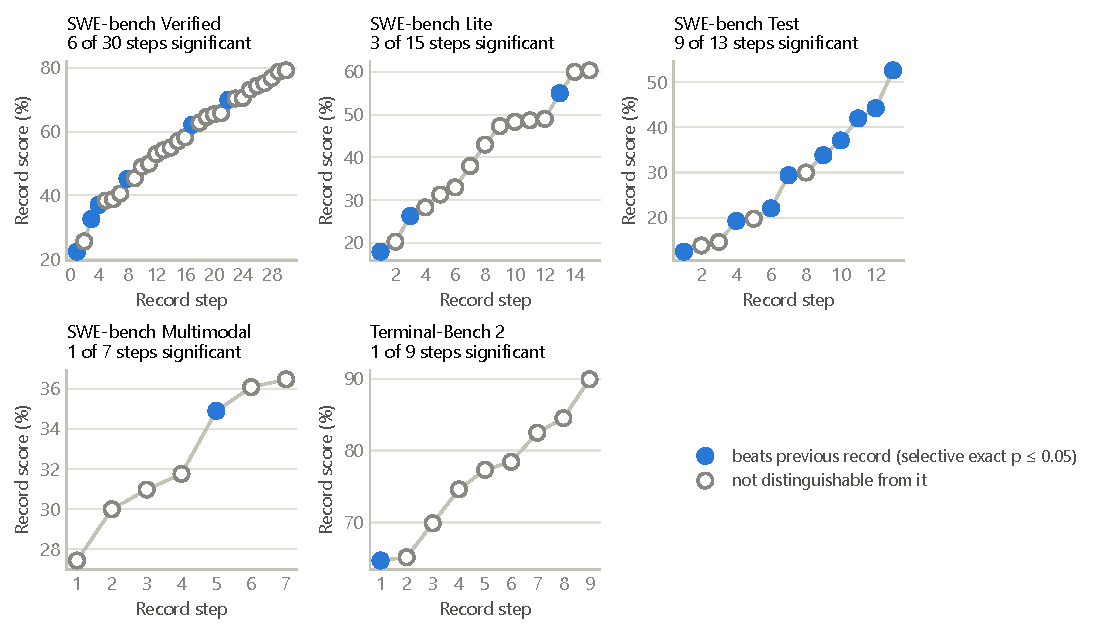
\includegraphics[width=\textwidth]{../figures/fig5_ladders.pdf}
\caption{The record ladders of five leaderboards. A filled point can be told apart from the previous record (selective exact paired test at the 5\% level); a hollow point cannot.}
\label{fig:ladders}
\end{figure}

\section{Full validation tables}
\begin{table}[H]
\centering\small
\resizebox{\textwidth}{!}{\begin{tabular}{rlrrrr}
\toprule
Tasks & Step in the chain & Steps & selective & two-sided & one-sided \\
\midrule
300 & first (holder is the first submission) & 576 & 0.7\% & 0.7\% & 3.1\% \\
300 & second & 501 & 0.2\% & 0.2\% & 0.8\% \\
300 & third and later & 621 & 0.0\% & 0.0\% & 0.2\% \\
500 & first (holder is the first submission) & 575 & 1.0\% & 1.0\% & 4.0\% \\
500 & second & 505 & 0.6\% & 0.6\% & 1.0\% \\
500 & third and later & 625 & 0.0\% & 0.0\% & 0.2\% \\
2,000 & first (holder is the first submission) & 578 & 2.1\% & 2.1\% & 4.8\% \\
2,000 & second & 506 & 0.4\% & 0.4\% & 1.6\% \\
2,000 & third and later & 729 & 0.0\% & 0.0\% & 0.1\% \\
\bottomrule
\end{tabular}
}
\caption{Global null: rejection rate by the step's position in the record chain. The first step compares against the first submission, conditioned only on no earlier record; later steps compare against a running maximum.}
\label{tab:position}
\end{table}

\begin{table}[H]
\centering\small
\resizebox{\textwidth}{!}{\begin{tabular}{rrrrrr}
\toprule
Tasks & 1 pt & 2 pts & 3 pts & 5 pts & Power at the formula's MDD \\
\midrule
300 & 0.05 & 0.13 & 0.27 & 0.67 & 0.77 (MDD 5.5 pts) \\
500 & 0.07 & 0.21 & 0.46 & 0.90 & 0.78 (MDD 4.2 pts) \\
2,000 & 0.23 & 0.72 & 0.98 & 1.00 & 0.77 (MDD 2.1 pts) \\
\bottomrule
\end{tabular}
}
\caption{Simulated power of the selective paired test for a true difference of 1, 2, 3 and 5 points, and at the minimum detectable difference given by the formula in Section~\ref{sec:methods}. Fitted Verified model, baseline score \NumSimBase\%.}
\label{tab:power}
\end{table}

\begin{table}[H]
\centering\small
\resizebox{0.9\textwidth}{!}{\begin{tabular}{rrrr}
\toprule
Tasks per benchmark & Winner is a truly best system (share of runs) & Set covers a truly best system when the winner is not & Median set size \\
\midrule
100 & 0.39 & 1.00 & 34 \\
250 & 0.65 & 1.00 & 19 \\
500 & 0.70 & 0.99 & 12 \\
\bottomrule
\end{tabular}
}
\caption{Known-truth simulation of ranking on SWE-bench Verified: how often the observed winner is a truly best system, and whether the confidence set covers a truly best system when it is not.}
\label{tab:lottery}
\end{table}

\begin{table}[H]
\centering\scriptsize
\resizebox{\textwidth}{!}{\begin{tabular}{llrrrrrrrr}
\toprule
Setting & Estimator & Mean error (SE) & Median error & RMSE & Coverage & Length & Defined & Mean, common & Median, common \\
\midrule
Known truth, 100 tasks & reported & +3.57 (0.19) & +3.80 & 5.25 & 0.83 & 15.1 & 100\% & +3.63 & +3.80 \\
 & bootstrap & +1.07 (0.21) & +1.00 & 4.26 & 0.88 & 14.0 & 100\% & +1.23 & +1.07 \\
 & iterated bootstrap & +0.65 (0.21) & +0.62 & 4.31 & 0.90 & 14.0 & 100\% & +0.86 & +0.81 \\
 & conditional & +2.51 (0.24) & +2.58 & 4.91 & 0.91 & 19.4 & 76\% & +2.51 & +2.58 \\
 & hybrid (AKM) & +2.51 (0.24) & +2.58 & 4.91 & 0.92 & 19.3 & 76\% & +2.51 & +2.58 \\
 & zoom interval (ZF) & +3.57 (0.19) & +3.80 & 5.25 & 0.96 & 24.9 & 100\% & +3.63 & +3.80 \\
\addlinespace
Known truth, 250 tasks & reported & +1.72 (0.12) & +1.60 & 2.92 & 0.89 & 9.9 & 100\% & +1.84 & +2.00 \\
 & bootstrap & +0.32 (0.13) & +0.26 & 2.54 & 0.93 & 9.2 & 100\% & +0.48 & +0.39 \\
 & iterated bootstrap & +0.13 (0.13) & +0.12 & 2.60 & 0.91 & 9.2 & 100\% & +0.31 & +0.26 \\
 & conditional & +0.80 (0.15) & +0.92 & 2.91 & 0.94 & 13.2 & 86\% & +0.80 & +0.92 \\
 & hybrid (AKM) & +0.80 (0.15) & +0.92 & 2.91 & 0.94 & 13.3 & 86\% & +0.80 & +0.92 \\
 & zoom interval (ZF) & +1.72 (0.12) & +1.60 & 2.92 & 0.99 & 15.5 & 100\% & +1.84 & +2.00 \\
\addlinespace
Known truth, 500 tasks & reported & +0.92 (0.08) & +1.00 & 1.85 & 0.94 & 7.0 & 100\% & +0.95 & +1.00 \\
 & bootstrap & +0.08 (0.09) & +0.04 & 1.71 & 0.95 & 6.6 & 100\% & +0.12 & +0.07 \\
 & iterated bootstrap & $-$0.02 (0.09) & $-$0.11 & 1.77 & 0.94 & 6.6 & 100\% & +0.03 & $-$0.09 \\
 & conditional & +0.05 (0.11) & +0.23 & 2.10 & 0.98 & 9.4 & 90\% & +0.05 & +0.23 \\
 & hybrid (AKM) & +0.05 (0.11) & +0.23 & 2.10 & 0.98 & 9.5 & 90\% & +0.05 & +0.23 \\
 & zoom interval (ZF) & +0.92 (0.08) & +1.00 & 1.85 & 0.99 & 10.8 & 100\% & +0.95 & +1.00 \\
\addlinespace
Equal leaders, 250 tasks & reported & +3.03 (0.11) & +2.75 & 3.75 & 0.81 & 10.2 & 100\% & +3.13 & +2.75 \\
 & bootstrap & +0.86 (0.12) & +0.65 & 2.56 & 0.92 & 9.2 & 100\% & +1.00 & +0.78 \\
 & iterated bootstrap & +0.43 (0.13) & +0.24 & 2.57 & 0.93 & 9.2 & 100\% & +0.60 & +0.41 \\
 & conditional & +1.20 (0.18) & +1.21 & 3.32 & 0.96 & 17.9 & 78\% & +1.20 & +1.21 \\
 & hybrid (AKM) & +1.20 (0.18) & +1.21 & 3.32 & 0.96 & 14.8 & 78\% & +1.20 & +1.21 \\
 & zoom interval (ZF) & +3.03 (0.11) & +2.75 & 3.75 & 0.97 & 16.5 & 100\% & +3.13 & +2.75 \\
\addlinespace
Equal leaders, 500 tasks & reported & +2.19 (0.08) & +2.15 & 2.70 & 0.83 & 7.3 & 100\% & +2.23 & +2.35 \\
 & bootstrap & +0.65 (0.08) & +0.67 & 1.81 & 0.93 & 6.6 & 100\% & +0.70 & +0.71 \\
 & iterated bootstrap & +0.35 (0.09) & +0.32 & 1.80 & 0.93 & 6.6 & 100\% & +0.41 & +0.39 \\
 & conditional & +0.30 (0.14) & +0.57 & 2.60 & 0.97 & 15.0 & 86\% & +0.30 & +0.57 \\
 & hybrid (AKM) & +0.30 (0.14) & +0.57 & 2.60 & 0.97 & 10.6 & 86\% & +0.30 & +0.57 \\
 & zoom interval (ZF) & +2.19 (0.08) & +2.15 & 2.70 & 0.99 & 11.6 & 100\% & +2.23 & +2.35 \\
\addlinespace
Held-out tasks & reported & +2.04 (0.16) & +2.40 & 4.06 & -- & 9.9 & 100\% & +2.14 & +2.40 \\
 & bootstrap & +0.52 (0.16) & +0.63 & 3.68 & -- & 9.2 & 100\% & +0.66 & +0.65 \\
 & iterated bootstrap & +0.30 (0.17) & +0.41 & 3.71 & -- & 9.2 & 100\% & +0.45 & +0.42 \\
 & conditional & +0.72 (0.20) & +0.94 & 4.12 & -- & 15.7 & 82\% & +0.72 & +0.94 \\
 & hybrid (AKM) & +0.72 (0.20) & +0.94 & 4.12 & -- & 14.2 & 82\% & +0.72 & +0.94 \\
 & zoom interval (ZF) & +2.04 (0.16) & +2.40 & 4.06 & -- & 15.7 & 100\% & +2.14 & +2.40 \\
\addlinespace
Held-out repositories (cluster, shift-adjusted) & reported & +3.48 (0.17) & +2.98 & 5.21 & -- & 9.9 & 100\% & +3.90 & +3.70 \\
 & bootstrap & +1.81 (0.18) & +1.59 & 4.34 & -- & 15.6 & 100\% & +2.22 & +2.13 \\
 & iterated bootstrap & +1.85 (0.18) & +1.97 & 4.48 & -- & 15.6 & 100\% & +2.24 & +2.37 \\
 & conditional & +3.38 (0.24) & +3.71 & 5.90 & -- & 13.1 & 82\% & +3.38 & +3.71 \\
 & hybrid (AKM) & +3.43 (0.23) & +3.71 & 5.82 & -- & 12.2 & 82\% & +3.43 & +3.71 \\
 & zoom interval (ZF) & +3.48 (0.17) & +2.98 & 5.21 & -- & 13.5 & 100\% & +3.90 & +3.70 \\
\addlinespace
Held-out repositories (cluster, unadjusted) & reported & +3.82 (0.26) & +3.05 & 6.96 & -- & 9.9 & 100\% & +3.68 & +2.69 \\
 & bootstrap & +2.14 (0.26) & +2.29 & 6.21 & -- & 15.6 & 100\% & +2.00 & +1.67 \\
 & iterated bootstrap & +2.18 (0.27) & +2.22 & 6.46 & -- & 15.6 & 100\% & +2.03 & +1.58 \\
 & conditional & +3.17 (0.31) & +2.01 & 7.12 & -- & 13.1 & 82\% & +3.17 & +2.01 \\
 & hybrid (AKM) & +3.22 (0.31) & +2.03 & 7.08 & -- & 12.2 & 82\% & +3.22 & +2.03 \\
 & zoom interval (ZF) & +3.82 (0.26) & +3.05 & 6.96 & -- & 13.5 & 100\% & +3.68 & +2.69 \\
\addlinespace
Held-out repositories (iid, shift-adjusted) & reported & +3.51 (0.17) & +3.04 & 5.22 & -- & 9.7 & 100\% & +3.90 & +3.75 \\
 & bootstrap & +2.13 (0.17) & +1.48 & 4.45 & -- & 9.1 & 100\% & +2.57 & +2.28 \\
 & iterated bootstrap & +1.98 (0.18) & +1.30 & 4.42 & -- & 9.1 & 100\% & +2.45 & +2.04 \\
 & conditional & +2.85 (0.22) & +2.23 & 5.21 & -- & 13.4 & 82\% & +2.85 & +2.23 \\
 & hybrid (AKM) & +2.85 (0.22) & +2.23 & 5.21 & -- & 13.0 & 82\% & +2.85 & +2.23 \\
 & zoom interval (ZF) & +3.51 (0.17) & +3.04 & 5.22 & -- & 15.2 & 100\% & +3.90 & +3.75 \\
\bottomrule
\end{tabular}
}
\caption{All validation settings on SWE-bench Verified. Columns as in Table~\ref{tab:valid}. The held-out-repository rows show the cluster-resampling corrections against the shift-adjusted and the unadjusted target, and the task-resampling (iid) corrections against the shift-adjusted target.}
\label{tab:valfull}
\end{table}

\begin{table}[H]
\centering\scriptsize
\resizebox{\textwidth}{!}{\begin{tabular}{llrrrrrrrr}
\toprule
Setting & Estimator & Mean error (SE) & Median error & RMSE & Coverage & Length & Defined & Mean, common & Median, common \\
\midrule
Known truth, 89 tasks & reported & +1.19 (0.11) & +1.12 & 2.90 & 0.85 & 9.2 & 100\% & +1.20 & +1.12 \\
 & bootstrap & $-$0.06 (0.12) & $-$0.03 & 2.97 & 0.85 & 9.2 & 100\% & $-$0.01 & +0.01 \\
 & iterated bootstrap & $-$0.10 (0.13) & $-$0.07 & 3.11 & 0.83 & 9.2 & 100\% & $-$0.03 & $-$0.03 \\
 & conditional & $-$0.18 (0.17) & +0.44 & 4.15 & 0.91 & 10.5 & 96\% & $-$0.18 & +0.44 \\
 & hybrid (AKM) & $-$0.13 (0.15) & +0.43 & 3.73 & 0.91 & 10.7 & 97\% & +0.01 & +0.44 \\
 & zoom interval (ZF) & +1.19 (0.11) & +1.12 & 2.90 & 0.95 & 14.1 & 100\% & +1.20 & +1.12 \\
\addlinespace
Equal leaders, 89 tasks & reported & +2.66 (0.10) & +2.47 & 3.65 & 0.82 & 10.8 & 100\% & +2.73 & +2.69 \\
 & bootstrap & +0.83 (0.11) & +0.60 & 2.79 & 0.90 & 10.0 & 100\% & +0.92 & +0.76 \\
 & iterated bootstrap & +0.44 (0.11) & +0.24 & 2.79 & 0.90 & 10.0 & 100\% & +0.55 & +0.34 \\
 & conditional & +0.50 (0.16) & +0.89 & 3.80 & 0.94 & 18.2 & 88\% & +0.50 & +0.89 \\
 & hybrid (AKM) & +0.53 (0.16) & +0.89 & 3.75 & 0.94 & 14.5 & 88\% & +0.53 & +0.89 \\
 & zoom interval (ZF) & +2.66 (0.10) & +2.47 & 3.65 & 0.95 & 16.0 & 100\% & +2.73 & +2.69 \\
\addlinespace
Held-out tasks & reported & +1.98 (0.23) & +1.59 & 5.98 & -- & 13.3 & 100\% & +1.91 & +1.12 \\
 & bootstrap & $-$0.71 (0.25) & $-$0.90 & 6.21 & -- & 13.7 & 100\% & $-$0.73 & $-$0.94 \\
 & iterated bootstrap & $-$1.15 (0.26) & $-$1.21 & 6.52 & -- & 13.7 & 100\% & $-$1.15 & $-$1.17 \\
 & conditional & $-$0.70 (0.32) & +0.12 & 7.72 & -- & 17.6 & 94\% & $-$0.70 & +0.12 \\
 & hybrid (AKM) & $-$0.48 (0.30) & +0.07 & 7.14 & -- & 16.7 & 95\% & $-$0.39 & +0.12 \\
 & zoom interval (ZF) & +1.98 (0.23) & +1.59 & 5.98 & -- & 20.8 & 100\% & +1.91 & +1.12 \\
\bottomrule
\end{tabular}
}
\caption{Validation on Terminal-Bench~2 (89 tasks, per-task rates from repeated trials; equal-leaders outcomes simulated with five trials).}
\label{tab:valtb}
\end{table}

\begin{table}[H]
\centering\scriptsize
\resizebox{\textwidth}{!}{\begin{tabular}{llrrrrrrrr}
\toprule
Setting & Estimator & Mean error (SE) & Median error & RMSE & Coverage & Length & Defined & Mean, common & Median, common \\
\midrule
Known truth, 318 questions & reported & +0.06 (0.11) & $-$0.01 & 2.12 & 0.94 & 8.1 & 100\% & +0.06 & $-$0.01 \\
 & bootstrap & $-$0.05 (0.11) & $-$0.03 & 2.22 & 0.93 & 7.9 & 100\% & $-$0.05 & $-$0.03 \\
 & iterated bootstrap & +0.08 (0.11) & +0.06 & 2.18 & 0.93 & 7.9 & 100\% & +0.08 & +0.06 \\
 & conditional & +0.06 (0.11) & $-$0.01 & 2.13 & 0.94 & 8.1 & 100\% & +0.06 & $-$0.01 \\
 & hybrid (AKM) & +0.06 (0.11) & $-$0.01 & 2.13 & 0.94 & 8.2 & 100\% & +0.06 & $-$0.01 \\
 & zoom interval (ZF) & +0.06 (0.11) & $-$0.01 & 2.12 & 0.99 & 12.1 & 100\% & +0.06 & $-$0.01 \\
\addlinespace
Equal leaders, 318 questions & reported & +3.88 (0.09) & +3.70 & 4.30 & 0.76 & 10.2 & 100\% & +3.96 & +4.01 \\
 & bootstrap & +1.03 (0.11) & +0.92 & 2.37 & 0.94 & 8.5 & 100\% & +1.14 & +0.93 \\
 & iterated bootstrap & +0.46 (0.12) & +0.27 & 2.35 & 0.95 & 8.5 & 100\% & +0.59 & +0.31 \\
 & conditional & $-$0.25 (0.24) & +0.62 & 4.54 & 0.97 & 24.1 & 87\% & $-$0.25 & +0.62 \\
 & hybrid (AKM) & $-$0.02 (0.23) & +0.62 & 4.22 & 0.97 & 14.6 & 87\% & $-$0.02 & +0.62 \\
 & zoom interval (ZF) & +3.88 (0.09) & +3.70 & 4.30 & 0.98 & 16.8 & 100\% & +3.96 & +4.01 \\
\addlinespace
Held-out questions & reported & $-$0.48 (0.21) & $-$0.66 & 4.22 & -- & 11.5 & 100\% & $-$0.48 & $-$0.66 \\
 & bootstrap & $-$0.97 (0.22) & $-$1.06 & 4.58 & -- & 11.5 & 100\% & $-$0.97 & $-$1.06 \\
 & iterated bootstrap & $-$0.62 (0.23) & $-$0.70 & 4.54 & -- & 11.5 & 100\% & $-$0.62 & $-$0.70 \\
 & conditional & $-$0.50 (0.21) & $-$0.67 & 4.25 & -- & 11.6 & 100\% & $-$0.50 & $-$0.67 \\
 & hybrid (AKM) & $-$0.50 (0.21) & $-$0.67 & 4.25 & -- & 11.8 & 100\% & $-$0.50 & $-$0.67 \\
 & zoom interval (ZF) & $-$0.48 (0.21) & $-$0.66 & 4.22 & -- & 18.0 & 100\% & $-$0.48 & $-$0.66 \\
\bottomrule
\end{tabular}
}
\caption{Validation on LiveBench (\NumLBT{} questions, per-question credit in $[0,1]$; equal-leaders outcomes simulated as pass or fail), \NumLBValR{} repetitions.}
\label{tab:vallb}
\end{table}
\end{document}
